%% src/build/template.tex — pandoc LaTeX template for build_paper.py
%% The whole document skeleton lives here so that page 1 (title + abstract +
%% keywords + DRAFT), page 2 (TOC) and the body are produced by ONE pandoc run
%% from ONE markdown input. Nothing here contains paper text.
\documentclass[11pt,a4paper]{article}

%% ---- build provenance, injected with -V buildmeta=... ----
% build=build_paper.py source=report/rendered.md source-sha256=c5cf631d327df4cedee02368fc480af5120e9dcd9937a6d4169197d6e2dd6245 pandoc-input=paper.pandoc.md pandoc-input-sha256=1b9c23a633221a143e12c567ba293b674eb1ee590851cb49f44aec35607092f6 header-sha256=0d35a9640f355225d95df79ac4512c7b2eb670ed0c9bbda69bd9e5a634cd3926 template-sha256=b1140b188bdc5e1864c6a052a243f991d16fd0661db4078e5cfe69322ebfa042 builder-sha256=40b0022f1fb964abd7bc525619415017098691b52ab75181cc50aef0572b8fe3 outdir=report preview=false number-sections=true wide-tables=wrap tables=15 claims=0 figures=9 generated-at=2026-10-27T03:07:19Z

%% src/build/header.tex — page/table/claim formatting for build_paper.py
%% Included verbatim via `pandoc --include-in-header`. Every setting here is a
%% LAYOUT setting only: no paper text, no numbers. If you change it, the builder
%% records a new sha256 in BUILD-INPUTS.json.
%%
%% Design constraints (batch brief):
%%   * no running headers anywhere; body pages show only a centred arabic page number
%%   * page 1 = title + abstract + keywords + DRAFT banner, page 2 = TOC; neither is numbered
%%   * anonymous (no author / team anywhere)
%%   * Chinese figure/table captions; Chinese section names
%%   * the paper source supplies its own section text, so numbering is decided by the
%%     pandoc template (`secnumdepth`), never by this header.

%% ---- fonts (system fonts; build_paper.py --check verifies availability) ----
\usepackage{fontspec}
\setmainfont{Times New Roman}
\setsansfont{Arial}
\setmonofont{Menlo}
\usepackage{xeCJK}
\setCJKmainfont{Songti SC}
\setCJKsansfont{Songti SC}
\setCJKmonofont{Songti SC}

%% ---- maths used by the paper source ----
\usepackage{amsmath}
\usepackage{amssymb}

%% ---- page geometry ----
\usepackage{geometry}
\geometry{a4paper,left=2.2cm,right=2.2cm,top=2.4cm,bottom=2.4cm,footskip=1.1cm}

%% ---- tables / figures / colour ----
\usepackage{calc}         % pandoc prose-table width expressions use \real{}
\usepackage{booktabs}      % \toprule \midrule \bottomrule (three-line tables)
\usepackage{longtable}     % tables that break across pages
\usepackage{array}         % p{} column helpers
\usepackage{graphicx}
\usepackage{lscape}        % landscape pages for the long wide appendix tables
\usepackage{rotating}     % sidewaystable for wide short tables
\usepackage{xcolor}
\usepackage{caption}       % \captionof so tables/figures stay in place (no float drift)

%% ---- Chinese caption and section names ----
\captionsetup{font=small,labelfont=bf,labelsep=quad,hypcap=false}
\renewcommand{\figurename}{图}
\renewcommand{\tablename}{表}
\renewcommand{\contentsname}{目录}
\renewcommand{\refname}{参考文献}
\renewcommand{\appendixname}{附录}
\renewcommand{\abstractname}{摘要}

%% ---- page style: NO running header, centred arabic footer number ----
%% `plain` = empty header + centred \thepage footer. The front matter switches
%% \thepage off through \pagenumbering{gobble}; the builder emits
%% \pagenumbering{arabic} right after the TOC, so body page 1 is the first body page.
\pagestyle{plain}
\AtBeginDocument{\pagenumbering{gobble}}

%% ---- typography ----
\setcounter{tocdepth}{2}
\setlength{\parindent}{2em}
\setlength{\parskip}{0.35em}
\setlength{\emergencystretch}{3em}
\setlength{\tabcolsep}{3pt}   % table p{} widths are computed for 2*3pt of padding
\renewcommand{\arraystretch}{1.12}
\setlength{\LTcapwidth}{\textwidth}

%% pandoc helpers expected by its LaTeX writer (mirrors its default template)
\providecommand{\tightlist}{%
  \setlength{\itemsep}{0pt}\setlength{\parskip}{0pt}}
\providecommand{\pandocbounded}[1]{#1}

%% Code points that Times New Roman lacks (U+2208 \in, U+2460..2462 circled digits,
%% U+FF5C fullwidth vertical bar) are typeset with the CJK font, which has them.
%% This changes the FONT, never the character or the number.
\xeCJKDeclareCharClass{CJK}{"2208,"2460,"2461,"2462,"FF5C}

%% ---- in-place table / figure containers ----
%% pandoc copies a raw LaTeX block verbatim only between a \begin{...} and its
%% matching \end{...}; these containers therefore wrap each generated float-free
%% table/figure so nothing sits outside the raw block.  No floats means tables stay
%% exactly where the text refers to them (no drift to the end of a section).
\newenvironment{bptable}{%
  \par\medskip\noindent\begin{minipage}{\linewidth}\centering
}{%
  \end{minipage}\par\medskip
}
\newenvironment{bpfigure}{%
  \par\medskip\noindent\begin{minipage}{\linewidth}\centering
}{%
  \end{minipage}\par\medskip
}
%% longtable font wrappers: font switches must be active BEFORE \begin{longtable},
%% because booktabs/longtable rules may only appear at a row boundary.
\newenvironment{bpLTsmall}{\small\renewcommand{\arraystretch}{1.02}}{}
\newenvironment{bpLTfootnotesize}{\footnotesize\renewcommand{\arraystretch}{1.02}}{}
\newenvironment{bpLTscriptsize}{\scriptsize\renewcommand{\arraystretch}{1.05}}{}

%% ---- hyperlinks: the rendered source carries DOIs / URLs as markdown links ----
%% (pandoc emits \href for those; without hyperref they are undefined control sequences)
\usepackage[hidelinks,breaklinks]{hyperref}
\hypersetup{unicode=true,pdfcreator={build-paper.py}}

%% ---- conditional fitting for wide display equations ----
%% The source has a couple of display equations slightly wider than the text
%% block; they are scaled down only when they are actually too wide.  The maths
%% symbols themselves are unchanged -- only the size of an over-wide line.
\newsavebox{\bpMathBox}
\newcommand{\bpMathFit}[1]{%
  \sbox{\bpMathBox}{$\displaystyle #1$}%
  \ifdim\wd\bpMathBox>\linewidth
    \resizebox{\linewidth}{!}{\usebox{\bpMathBox}}%
  \else
    \usebox{\bpMathBox}%
  \fi
}

%% ---- evidence-registry block (the eight claim-placeholder registrations) ----
%% Small font, framed, light background: visually distinct from prose without
%% deleting or reordering any claim text.
\newsavebox{\bpEvidBox}
\newenvironment{evidenceregistry}{%
  \par\medskip\noindent
  \setlength{\fboxsep}{5pt}\setlength{\fboxrule}{0.4pt}%
  \begin{lrbox}{\bpEvidBox}%
  \begin{minipage}{\dimexpr\linewidth-2\fboxsep-2\fboxrule\relax}%
  \small\setlength{\parindent}{0pt}\setlength{\parskip}{2pt}%
}{%
  \end{minipage}%
  \end{lrbox}%
  \noindent\fcolorbox{black!30}{black!4}{\usebox{\bpEvidBox}}%
  \par\medskip
}

%% ---- table note (the `注：...` paragraph of every table block) ----
\newenvironment{tablenote}{%
  \par\smallskip\noindent\footnotesize
  \setlength{\parindent}{0pt}\setlength{\parskip}{0pt}%
  \raggedright
}{%
  \par\medskip
}

%% ---- DRAFT banner (page 1) ----
\newsavebox{\bpDraftBox}
\newenvironment{draftbanner}{%
  \par\medskip\noindent
  \setlength{\fboxsep}{5pt}\setlength{\fboxrule}{0.4pt}%
  \begin{lrbox}{\bpDraftBox}%
  \begin{minipage}{\dimexpr\linewidth-2\fboxsep-2\fboxrule\relax}%
  \small\setlength{\parindent}{0pt}\setlength{\parskip}{0pt}%
  \raggedright
}{%
  \end{minipage}%
  \end{lrbox}%
  \noindent\fcolorbox{black!45}{yellow!8}{\usebox{\bpDraftBox}}%
  \par\medskip
}
%% ---- display-only tightening (preview-D): never changes content or FIG bytes ----
\setlength{\textfloatsep}{6pt plus 2pt minus 2pt}
\setlength{\floatsep}{4pt plus 1pt minus 1pt}
\setlength{\intextsep}{5pt plus 2pt minus 2pt}
\setlength{\abovecaptionskip}{3pt}
\setlength{\belowcaptionskip}{0pt}
\setkeys{Gin}{height=0.23\textheight,keepaspectratio}
\renewcommand{\arraystretch}{0.90}
\AtBeginEnvironment{longtable}{\small}
\setlength{\abovedisplayskip}{4pt plus 1pt}
\setlength{\belowdisplayskip}{4pt plus 1pt}
\setlength{\abovedisplayshortskip}{2pt}
\setlength{\belowdisplayshortskip}{2pt}
\setlength{\parskip}{0pt}
\setlength{\topsep}{2pt plus 1pt}
\setlength{\partopsep}{0pt}
%% ---- end display-only tightening ----

%% Section numbering is controlled by LaTeX `secnumdepth`, not by the source:
%%   * default (no --number-sections): secnumdepth = -\maxdimen  -> headings are
%%     printed exactly as written (use this when the source carries manual numbers)
%%   * --number-sections: LaTeX numbers 1, 1.1, ... (摘要 stays \section*)
\setcounter{secnumdepth}{2}

\title{基于稳健表示、共表达网络与风格条件生成的啤酒化合物---感官强度建模}
\author{}
\date{}

\begin{document}
\maketitle
\thispagestyle{empty}
\section*{摘要}\label{ux6458ux8981}
\addcontentsline{toc}{section}{摘要}

\begin{draftbanner}
\textbf{DRAFT——科学证据与交付限制见文末，非最终提交版。} 本文是论文源的工作稿：全部数字均取自项目台账中真实执行、尚未过期的确认轮实验，或由这些产物脚本生成的表格；正文结论尚未通过交付门禁，不得作为最终提交稿或对外结果引用。
\end{draftbanner}

针对啤酒化学谱与感官强度之间的高维、非线性关联，以及风格样本不均衡和缺陷控制要求，本文以
250 款啤酒的 231 个化学及理化变量与 50
个标准化感官标签为基础，建立预测、关联识别与风格条件生成的统一框架，并在每一问内先固定评价协议、再比较候选。

问题一在训练折内完成缺失处理与稳健表示，比较逐目标训练中位数、普通
Ridge、图 Ridge
与图正则低秩四种模型，四者共用同一嵌套交叉验证、同一预处理规则与同一截距约定。主候选的
Aroma/Flavour 30 维等权平均绝对误差为
0.35929156588219174，同一协议下的逐目标中位数基线为
0.39817732837288883；全部 50 维的平均绝对误差为
0.350504156920024，中位数基线为
0.3918800487369867。全部预测均为折外预测：任一啤酒的预测都不由包含该啤酒的训练行产生。0--6
等级由训练折标签的中点经验分布函数标定，只是训练分布内的相对等级，不恢复原始人工评分。

问题二把候选宇宙拆为 216 个严格单体化合物与 15 个扩展指标两张表，用总体
Spearman、风格内残差化
Spearman、图低秩回归系数与三者百分位均值四种方法，经风格分层 bootstrap
给出逐维 Top-3。四种方法 Top-3 的平均两两 Jaccard 为
0.2091111111111111，说明方法间集合一致性有限；该量是集合一致性，不是识别准确率，附件交叉相关表与本研究同源，只作同源对照。

问题三把生成与迁移分开评价。生成侧采用含编码质量点的层次收缩边际与收缩高斯
Copula，在约束投影后给出非负物理浓度设计谱；归一化经验 V 能量距离为
0.8840256215416039，而同样本量的源样本重采样参照更低（表
q3-quality），因此本文不宣称生成分布优于重采样参照。迁移侧在声明的凸二次规划下求解，198
个求解证书均报告最优，综合不增率（四条化学列与代理上限的合计口径）为
1；该值由硬上界构造保证并已饱和，不作为稳健性证据，也不报告``迁移准确率''。

稳健性检验按问题分列：种子扰动、参数扰动与预算扰动的相对极差均在各自预注册限内，但每项只覆盖三个冻结种子中的两个，且固定种子的独立复跑只证明确定性重现，不是独立实现。问题一的划分完整性与留出评价、问题三的原生优化检查属结构性不可满足，相应选择状态保持为草稿选择。

\textbf{关键词：} 图正则低秩回归；嵌套交叉验证；风格混杂；分层
bootstrap；收缩 Copula；凸二次规划证书

\newpage
\thispagestyle{empty}
\tableofcontents
\newpage
\pagenumbering{arabic}

\section{问题重述与分析}\label{ux95eeux9898ux91cdux8ff0ux4e0eux5206ux6790}

\subsection{题目要求与建模对象}\label{ux9898ux76eeux8981ux6c42ux4e0eux5efaux6a21ux5bf9ux8c61}

赛题要求从化学特征出发完成三项相互关联的任务：一是估计评分卡定义的 Aroma
与 Flavour 感官强度，并输出 0--6
分级；二是利用化合物相关矩阵构建共表达图，识别每个感官维度的 Top-3
关键因素，并论证其稳定性与化学合理性；三是学习以
\texttt{tasting\_category\_fine} 为条件的化合物谱生成模型，展示
Tripel、Kriek、Lambic 等风格的感官画像，并将 Pils/Lager 化学谱迁移至
Tripel，同时控制指定缺陷 {[}1{]}。

三问的共同难点在于：特征数接近样本量，化合物之间高度相关；标准化感官值与原始整数评分之间缺少可逆标定；风格差异可能使总体相关偏离风格内关系；小样本风格难以独立估计高维联合分布。本文的做法是先核实数据尺度与编码规则，再为每一问固定评价协议，最后在该协议下比较候选。

{
\begin{longtable}[]{@{}
  >{\raggedright\arraybackslash}p{(\linewidth - 6\tabcolsep) * \real{0.2500}}
  >{\raggedright\arraybackslash}p{(\linewidth - 6\tabcolsep) * \real{0.2500}}
  >{\raggedright\arraybackslash}p{(\linewidth - 6\tabcolsep) * \real{0.2500}}
  >{\raggedright\arraybackslash}p{(\linewidth - 6\tabcolsep) * \real{0.2500}}@{}}
\toprule\noalign{}
\begin{minipage}[b]{\linewidth}\raggedright
任务
\end{minipage} & \begin{minipage}[b]{\linewidth}\raggedright
建模对象
\end{minipage} & \begin{minipage}[b]{\linewidth}\raggedright
核心输出
\end{minipage} & \begin{minipage}[b]{\linewidth}\raggedright
主要评价
\end{minipage} \\
\midrule\noalign{}
\endhead
\bottomrule\noalign{}
\endlastfoot
感官评分 & \(Y=f(X)+E\) & 折外连续预测与 0--6 相对分级 & 30 维与 50
维等权平均 MAE、平均 \(R^2\)、Skill \\
关键因素 & 化学成分与感官的同期关联 & 每个维度 3 个候选及其稳定性 &
入选频率、方法间 Jaccard \\
生成与迁移 & \(p(X\mid s)\) 与声明模型下的迁移算子 &
风格谱、感官画像、缺陷对照 & 能量距离、约束满足率、求解证书 \\
\end{longtable}
}

\subsection{三问的评价对象与证据边界}\label{ux4e09ux95eeux7684ux8bc4ux4ef7ux5bf9ux8c61ux4e0eux8bc1ux636eux8fb9ux754c}

本文严格区分四类陈述：\textbf{已登记的计划}（验证协议、稳健性计划已登记）、\textbf{真实执行}（实验状态为成功，退出码、结果文件与指标真实存在）、\textbf{验证通过}（对应检查项通过且未过期）、\textbf{被选为最终方案}（选择记录与冻结身份一致）。四者不可互相替代。

按此口径，本轮三问的证据状态并不相同，正文与文末限制按实际状态书写，不做统一化表述：

\begin{itemize}
\tightlist
\item
  问题一的对照、分组、折间与逐风格结果均来自真实执行的折外实验，泄漏检查、基线比较检查与固定种子独立复跑三项已通过；但该问没有留出集、也没有登记数据划分，划分完整性与留出评价两项检查结构性不可满足，因此选择状态只到草稿选择。
\item
  问题二的泄漏检查与固定种子独立复跑已通过，选择状态为已验证；但``稳定性''与``集合一致性''不等于识别准确率，附件交叉相关表与本研究同源。
\item
  问题三的生成与迁移是两个不同对象，各自有独立指标与验证；生成侧的泄漏检查与复跑已通过，迁移侧的不增率检查与复跑已通过；原生的优化可行性与优化目标检查因实验未声明优化参数而被工具具名拒绝，本文不声称通过。单一选择字段无法同时表示两个对象，选择状态为草稿选择。
\end{itemize}

\subsection{与附件实际结构不符的三处修正}\label{ux4e0eux9644ux4ef6ux5b9eux9645ux7ed3ux6784ux4e0dux7b26ux7684ux4e09ux5904ux4feeux6b63}

第一，评分工作簿是空白评分卡。附件 \texttt{3.xlsx} 含 \texttt{beer\_1}
至 \texttt{beer\_12} 与一张汇总页，各页均为带 0--6
刻度的空白模板，不含已填写的原始整数评分，也不含该量表的标定参数。因此本文的
0--6 等级只能定义为可复核的相对等级，而不能声称恢复了人工评分。

第二，交叉相关表的感官列顺序与主表不一致。附件 \texttt{6.csv}
尾部的列序为 Carbonation、Aftertaste、Body、Overall，而目标表为
aftertaste、body、co2、overall
的顺序，按位置对齐会错位三列，并连带使化学行与候选索引错配。本文改为按名称一对一对齐：化学行经化学元数据映射到特征名，感官列经
50
条字面字典映射到目标名，任何重复、歧义或未匹配的行按名报告并中止，不做静默丢弃。

第三，先导轮实现存在三处名实不符，本轮全部重做。其一是``普通
Ridge''实际带有图正则，不是普通 Ridge；其二是低秩拟合每轮刷新截距而
Ridge
参照固定标签均值，两者不在同一截距约定下可比；其三是``折外''表把样本内预测与留出预测混在同一张表里。确认轮把四模型放在同一嵌套协议、同一预处理规则与同一截距公式下重算，并对``秩
50 且 \(\gamma=0\) 应还原普通 Ridge''作逐折数值核对。

\section{数据核实与统一字典}\label{ux6570ux636eux6838ux5b9eux4e0eux7edfux4e00ux5b57ux5178}

\subsection{样本对齐与主键}\label{ux6837ux672cux5bf9ux9f50ux4e0eux4e3bux952e}

化学表、感官表与跨来源描述符表均按 \texttt{beer} 序号连接：\texttt{beer}
是 1..250 的置换，可整行对齐 1.csv 与 4.csv；后两表的 \texttt{beer\_id}
只有 96 个唯一值，存在截断，不能作为可靠连接键。化学表规模为 250 行、231
列，感官表 50 列，风格变量共 22 类。

\subsection{尺度、编码点与物理浓度}\label{ux5c3aux5ea6ux7f16ux7801ux70b9ux4e0eux7269ux7406ux6d53ux5ea6}

利用附件校准表覆盖的 70 个变量逐列回算，37 列与 \(\log_{10}c\) 一致，33
列与原始浓度 \(c\) 一致，其余 161
列缺少直接校准依据。在已确认的对数列中，\(x<0\)、\(x=0\)、\(x>0\)
分别对应以指定单位计量的
\(0<c<1\)、\(c=1\)、\(c>1\)；该逻辑不适用于未经确认的列。

37 个对数列中有 755
个单元格对应校准表记录的零值，其存储值为该列最小正浓度一半的
\(\log_{10}\)。另有 142 个未校准列共享约 \(-1.8178\) 的地板编码，合计
6807
个单元格。这些数值首先表示观测编码，不能据此断言真实浓度为零或已知低于某个仪器检出限。生成模型因此显式保留地板质量点，物理阈值比较只在尺度与单位已确认时进行。

{
\begin{longtable}[]{@{}
  >{\raggedright\arraybackslash}p{(\linewidth - 4\tabcolsep) * \real{0.3000}}
  >{\raggedleft\arraybackslash}p{(\linewidth - 4\tabcolsep) * \real{0.4000}}
  >{\raggedright\arraybackslash}p{(\linewidth - 4\tabcolsep) * \real{0.3000}}@{}}
\toprule\noalign{}
\begin{minipage}[b]{\linewidth}\raggedright
数据类别
\end{minipage} & \begin{minipage}[b]{\linewidth}\raggedleft
数量
\end{minipage} & \begin{minipage}[b]{\linewidth}\raggedright
用途及处理
\end{minipage} \\
\midrule\noalign{}
\endhead
\bottomrule\noalign{}
\endlastfoot
已校准 log10 变量 & 37 & 预测时使用存储值；物理比较时反变换
\(c=10^x\) \\
已校准线性变量 & 33 & 保留原单位；物理比较时施加非负下界 \\
未直接校准变量 & 161 & 以存储尺度建模，只在声明的观测支撑内取值 \\
其中派生汇总量 & 5（含于上两行，不另计） &
热量、总酸、总酯、酒花香气及硫化物汇总；属子集，合计仍为 231 \\
感官目标 & 50 & 用于预测与评价，不作为生成器的化学输入 \\
\end{longtable}
}

\subsection{缺失处理与两套评价协议}\label{ux7f3aux5931ux5904ux7406ux4e0eux4e24ux5957ux8bc4ux4ef7ux534fux8bae}

化学表有 73 个缺失单元格，分布于 9 列、63 行，其中乙酸戊酯 27
个、酒花香气汇总 13 个、甲基吡嗪 12 个、双乙酰 9 个、3-甲基丁醛 7
个，其余 4 列合计 5 个。预测模型在当前训练折内部进行中位数填补，并增加 9
个缺失指示列；验证折与评价行沿用训练折参数。生成模型估计边际时只使用有效观测，不把填补值的堆积当作真实概率质量点。

本轮存在两套并行的评价协议，正文不把它们混为一谈：

\begin{itemize}
\tightlist
\item
  \textbf{问题一采用全样本嵌套交叉验证}：3 次重复 × 3 个外层折 × 每折 3
  个内层折，覆盖全部 250 款啤酒，每次重复的折外预测合起来恰好覆盖 250
  行，三次重复合计 750
  行预测。该协议没有任何留出集，因此``留出泛化''类陈述在本文中不成立。
\item
  \textbf{问题二使用注册的 200 行训练集}：保留的 50
  行在本轮不参与拟合，也不用于评价，只是为控制重复曝光而保留。问题二的
  bootstrap 只在该 200 行内进行。
\end{itemize}

两套协议的对象不同，其误差数值不可横向比较。

\subsection{防止信息泄露}\label{ux9632ux6b62ux4fe1ux606fux6cc4ux9732}

缺失处理、稳健表示、目标中心化、图估计、超参数选择与分级切点全部在训练折内拟合。任一啤酒的折外预测都来自不含该啤酒的训练集：外层测试行不参与填补中位数、不参与标准化参数、不参与图估计、不参与内层选参、不参与分级切点。附件化学相关矩阵来源于全部
250
款啤酒，本轮只用于说明网络来源，未作为独立网络产物重算；预测与关联模型的正则化图必须由当前训练折重新计算。跨来源感官描述符与附件提供的既有模型重要性均不作为化学输入。

\section{模型假设、符号与总体框架}\label{ux6a21ux578bux5047ux8bbeux7b26ux53f7ux4e0eux603bux4f53ux6846ux67b6}

\subsection{主要假设}\label{ux4e3bux8981ux5047ux8bbe}

第一，已对齐的同期样本可用于估计本数据分布内的化学---感官关系；该关系不直接代表未来批次或其他市场。第二，可确认尺度的变量按校准字典解释，未校准变量仅作为存储尺度上的观测量。第三，风格内秩残差可减少风格组间差异的影响，但不能消除未观测混杂。第四，条件生成模型近似描述既有风格的观测分布；缺陷约束是数学筛查规则，不能单独保证真实啤酒的工艺可实现性。第五，迁移结论只在声明的变量空间、目标函数与约束集合下成立。

\subsection{符号说明}\label{ux7b26ux53f7ux8bf4ux660e}

{
\begin{longtable}[]{@{}
  >{\raggedright\arraybackslash}p{(\linewidth - 2\tabcolsep) * \real{0.5000}}
  >{\raggedright\arraybackslash}p{(\linewidth - 2\tabcolsep) * \real{0.5000}}@{}}
\toprule\noalign{}
\begin{minipage}[b]{\linewidth}\raggedright
符号
\end{minipage} & \begin{minipage}[b]{\linewidth}\raggedright
含义
\end{minipage} \\
\midrule\noalign{}
\endhead
\bottomrule\noalign{}
\endlastfoot
\(X\in\mathbb R^{n\times p}\) & 存储尺度化学及理化特征，\(p=231\) \\
\(Z\) & 当前训练折拟合的稳健表示，含 9 个缺失指示列，共 240 维 \\
\(Y\in\mathbb R^{n\times q}\) & 标准化感官标签，\(q=50\)；Aroma 与
Flavour 各 15 维记作 \(q_{AF}=30\) \\
\(s_i\) & 第 \(i\) 款啤酒的细粒度风格，共 22 类 \\
\(G=(V,E,W),L_G\) & 训练折内估计的带符号关联图及其拉普拉斯矩阵 \\
\(B,r\) & 多输出回归系数及秩约束 \\
\(\rho^{\mathrm{total}},\rho^{\mathrm{within}}\) &
总体及风格内残差化秩相关 \\
\(\pi_{jt},S_{jt}\) & 候选 \(j\) 在维度 \(t\) 的入选频率与综合分 \\
\(F_{j,s},R_s\) & 风格条件边际分布与 Copula 相关矩阵 \\
\(c_j,T_j\) & 已确认单位的物理浓度与感官阈值 \\
\(z\) & 迁移二次规划的变量，为折叠标准化存储空间中的 231 维向量 \\
\end{longtable}
}

\subsection{总体框架}\label{ux603bux4f53ux6846ux67b6}

统一框架以字典为基础：问题一估计多输出感官预测器并给出相对分级；问题二使用同族图低秩回归的系数，与总体关联和风格内关联共同识别候选；问题三先条件生成化学谱，再在声明的凸二次规划下做风格迁移。三问共享标签体系与化学字典，但评价对象不同：问题一评价逐维误差，问题二评价集合一致性，问题三评价分布距离与求解证书。任何跨问的``综合得分''在本文中都不使用。

\section{问题一：图正则低秩预测与相对分级}\label{ux95eeux9898ux4e00ux56feux6b63ux5219ux4f4eux79e9ux9884ux6d4bux4e0eux76f8ux5bf9ux5206ux7ea7}

\subsection{训练折内稳健表示}\label{ux8badux7ec3ux6298ux5185ux7a33ux5065ux8868ux793a}

231 个化学特征与 9 个缺失指示列构成 240
维输入。对化学变量比较两种表示：存储尺度 z 分数与 Rank-Gauss 表示。

\[\bpMathFit{
z_{ij}^{\mathrm{zs}}=\operatorname{clip}\!\left(\frac{x_{ij}-\mu_{j,\mathrm{train}}}{s_{j,\mathrm{train}}},\,-8,\,8\right),
\qquad
u_{ij}=\widehat F_{j,\mathrm{train}}(x_{ij}),\quad
z_{ij}^{\mathrm{rg}}=\Phi^{-1}\{\operatorname{clip}(u_{ij},\varepsilon,1-\varepsilon)\},\quad
\varepsilon=(2n_{\mathrm{train}})^{-1}.
}\]

z 分数按冻结规则截断在
\(\pm8\)，避免单个极端值主导最小二乘；截断只发生在表示层，不改变原始浓度。重复观测使用中秩，验证样本沿用训练经验分布。目标按训练折均值和标准差变换为
\(\widetilde y_{it}=(y_{it}-\mu_t)/s_t\)；近零标准差置为
1，以避免数值发散。

\subsection{图正则低秩多输出回归}\label{ux56feux6b63ux5219ux4f4eux79e9ux591aux8f93ux51faux56deux5f52}

模型同时利用感官维度之间的共享结构及化学变量的共线性，求解

\[\bpMathFit{
\min_{B,b}\ \frac{1}{n_{\mathrm{train}}}\|\widetilde Y-ZB-\mathbf1b^\top\|_F^2
+\lambda\|B\|_F^2+\gamma\operatorname{tr}(B^\top L_GB),\qquad \operatorname{rank}(B)\le r.
}\]

训练图的边权为
\(w_{jk}=\widehat\rho_{jk}\mathbf1\{|\widehat\rho_{jk}|\ge\tau\}\)，\(w_{jj}=0\)，其中
\(\tau=0.5\) 在任何拟合之前冻结；\(\widehat\rho\) 由训练折的中秩
Spearman 计算。取 \(L_G=D_{|W|}-W\)，其惩罚可写为

\[\bpMathFit{
\operatorname{tr}(B^\top L_GB)=\frac12\sum_{j,k}|w_{jk}|\|B_{j\cdot}-\operatorname{sign}(w_{jk})B_{k\cdot}\|_2^2 .
}\]

正相关变量倾向具有相近系数，负相关变量倾向具有反向系数。\(D_{|W|}-W\) 由
Gershgorin 圆盘定理保证半正定（特征值位于
\([0,\,2\max_i\sum_j|w_{ij}|]\)），因此实现中不再对特征值作截断；缺失指示列的图惩罚块设为零。

低秩解取闭式形式而非迭代近似：令 \(Z_c,\widetilde Y_c\)
为训练块的中心化矩阵，

\[\bpMathFit{
A=\frac{1}{n}Z_c^\top Z_c+\lambda I+\gamma L_G,\qquad C=\frac{1}{n}Z_c^\top \widetilde Y_c,\qquad
B=A^{-1}CV_rV_r^\top,
}\]

其中 \(V_r\) 为 \(C^\top A^{-1}C\) 的前 \(r\)
个特征向量。该解是有秩约束问题的精确最小化点，\(r=q\)
时退化为满秩惩罚解；实现只做 Cholesky 分解与三角回代，不显式求逆。

四个线性模型统一使用同一截距公式

\[\bpMathFit{
b=\bar y-\bar z\,B,\qquad \widehat y=\bar y+(z-\bar z)B,
}\]

其中 \(\bar z,\bar y\) 为训练块均值。该约定使``秩 50 且
\(\gamma=0\)''必须还原普通 Ridge；逐折核对的最大预测差为
3.9968028886505635e-15，机器精度通过。

\subsection{四个同协议模型与内层选参}\label{ux56dbux4e2aux540cux534fux8baeux6a21ux578bux4e0eux5185ux5c42ux9009ux53c2}

同一进程中运行四个模型，预处理规则、截距约定、外层划分与分级切点完全一致：

{
\begin{longtable}[]{@{}
  >{\raggedright\arraybackslash}p{(\linewidth - 4\tabcolsep) * \real{0.3333}}
  >{\raggedright\arraybackslash}p{(\linewidth - 4\tabcolsep) * \real{0.3333}}
  >{\raggedright\arraybackslash}p{(\linewidth - 4\tabcolsep) * \real{0.3333}}@{}}
\toprule\noalign{}
\begin{minipage}[b]{\linewidth}\raggedright
模型
\end{minipage} & \begin{minipage}[b]{\linewidth}\raggedright
定义
\end{minipage} & \begin{minipage}[b]{\linewidth}\raggedright
内层搜索
\end{minipage} \\
\midrule\noalign{}
\endhead
\bottomrule\noalign{}
\endlastfoot
逐目标训练中位数 & 每维取外层训练标签的中位数 & 无参数 \\
普通 Ridge & \(\gamma=0\)，\(r=50\)（无秩约束） & 表示、\(\lambda\) \\
图 Ridge & \(\gamma>0\)，\(r=50\) &
表示、\(\lambda\)、\(\gamma\in\{0.1,1\}\) \\
图正则低秩 & \(\gamma\ge0\)，\(r\in\{3,6,10\}\) &
表示、\(\lambda\)、\(\gamma\in\{0,0.1,1\}\)、\(r\) \\
\end{longtable}
}

\(\lambda\) 的网格为 \(\{0.1,1,10\}\)，表示在 z 分数与 Rank-Gauss
之间选择。每个外层训练集内部再切 3
个内层折选参，内层网格的每一个单元都写入实验目录，使参数选择可逐格复核。外层评价使用
3 次重复 × 3 个外层折，重复种子在协议中冻结。

\subsection{预测结果：同协议四模型对照}\label{ux9884ux6d4bux7ed3ux679cux540cux534fux8baeux56dbux6a21ux578bux5bf9ux7167}

\begin{bptable}
\setcounter{table}{0}
%% table-id: q1-models sha256:89369169d05f5d7d0901a347096f00fd3edacfeacbc822adf1eb72965d39ace9
\captionof{table}{同一嵌套协议下四种模型的预测误差}\label{tab:q1-models}
\par\smallskip
\small
\resizebox{\linewidth}{!}{%
\begin{tabular}{@{}lrrrrrr@{}}
\toprule
模型 & A/\allowbreak{}F30 等权 MAE & 全 50 维 MAE & 宏平均 R²（A/\allowbreak{}F30） & Skill（A/\allowbreak{}F30） & 相对中位数差值（A/\allowbreak{}F30） & 相对中位数差值（全 50 维） \\
\midrule
最小中位数基线 & 0.3982 & 0.3919 & -0.0584 & 0.0000 & 0.0000 & 0.0000 \\
普通 Ridge & 0.3667 & 0.3582 & 0.1584 & 0.0791 & -0.0791 & -0.0860 \\
图 Ridge & 0.3664 & 0.3575 & 0.1576 & 0.0798 & -0.0798 & -0.0879 \\
图正则低秩 & 0.3593 & 0.3505 & 0.1854 & 0.0977 & -0.0977 & -0.1056 \\
\bottomrule
\end{tabular}
}%
\begin{tablenote}注：三次重复 × 三次外折的折外池化结果；A/F30 为香气 15 维与风味 15 维的等权平均，“全 50 维”另加其余 20 维。Skill（A/F30）= 1 − MAE / 中位数基线 MAE；相对中位数差值 =（本模型 MAE − 中位数基线 MAE）/ 中位数基线 MAE，负值表示优于基线。普通 Ridge 固定无图惩罚（γ=0）且不含低秩项；图 Ridge 不含低秩项；图正则低秩的秩在 \{3, 6, 10\} 中由内层验证选参，图惩罚强度 γ 与正则强度 λ 的选参网格为 γ∈\{0, 0.1, 1\}、λ∈\{0.1, 1, 10\}。本表只描述同一协议下的相对拟合差异，不构成对任一分量的显著性结论。\end{tablenote}
\end{bptable}

同一协议下，中位数基线的 Aroma/Flavour 30 维等权 MAE 为
0.39817732837288883，全部 50 维为 0.3918800487369867。图正则低秩模型把
30 维 MAE 降到 0.35929156588219174，50 维降到 0.350504156920024；平均
\(R^2\) 由基线的负值转为 0.1854199218782663，汇总 Skill 为
0.09765940881064172。

本文使用两个 Skill 口径，二者不可混用：逐维
\(\mathrm{Skill}_t=1-\mathrm{MAE}_{t,\mathrm{model}}/\mathrm{MAE}_{t,\mathrm{median}}\)，以及汇总
\(\mathrm{Skill}=1-\overline{\mathrm{MAE}}_{\mathrm{model}}/\overline{\mathrm{MAE}}_{\mathrm{median}}\)。前者正负混杂时后者仍可为正，因此逐维
Skill 图与汇总值必须分别解读。

\begin{bpfigure}
%% figure-id: FIG-0032 sha256:2557001da5d9510a8f8afbfd682d4149c2b276b294901892dbc45ee0c8cf5838
%% figure-src: ../figures/confirmatory/Q1-per-target-skill.png
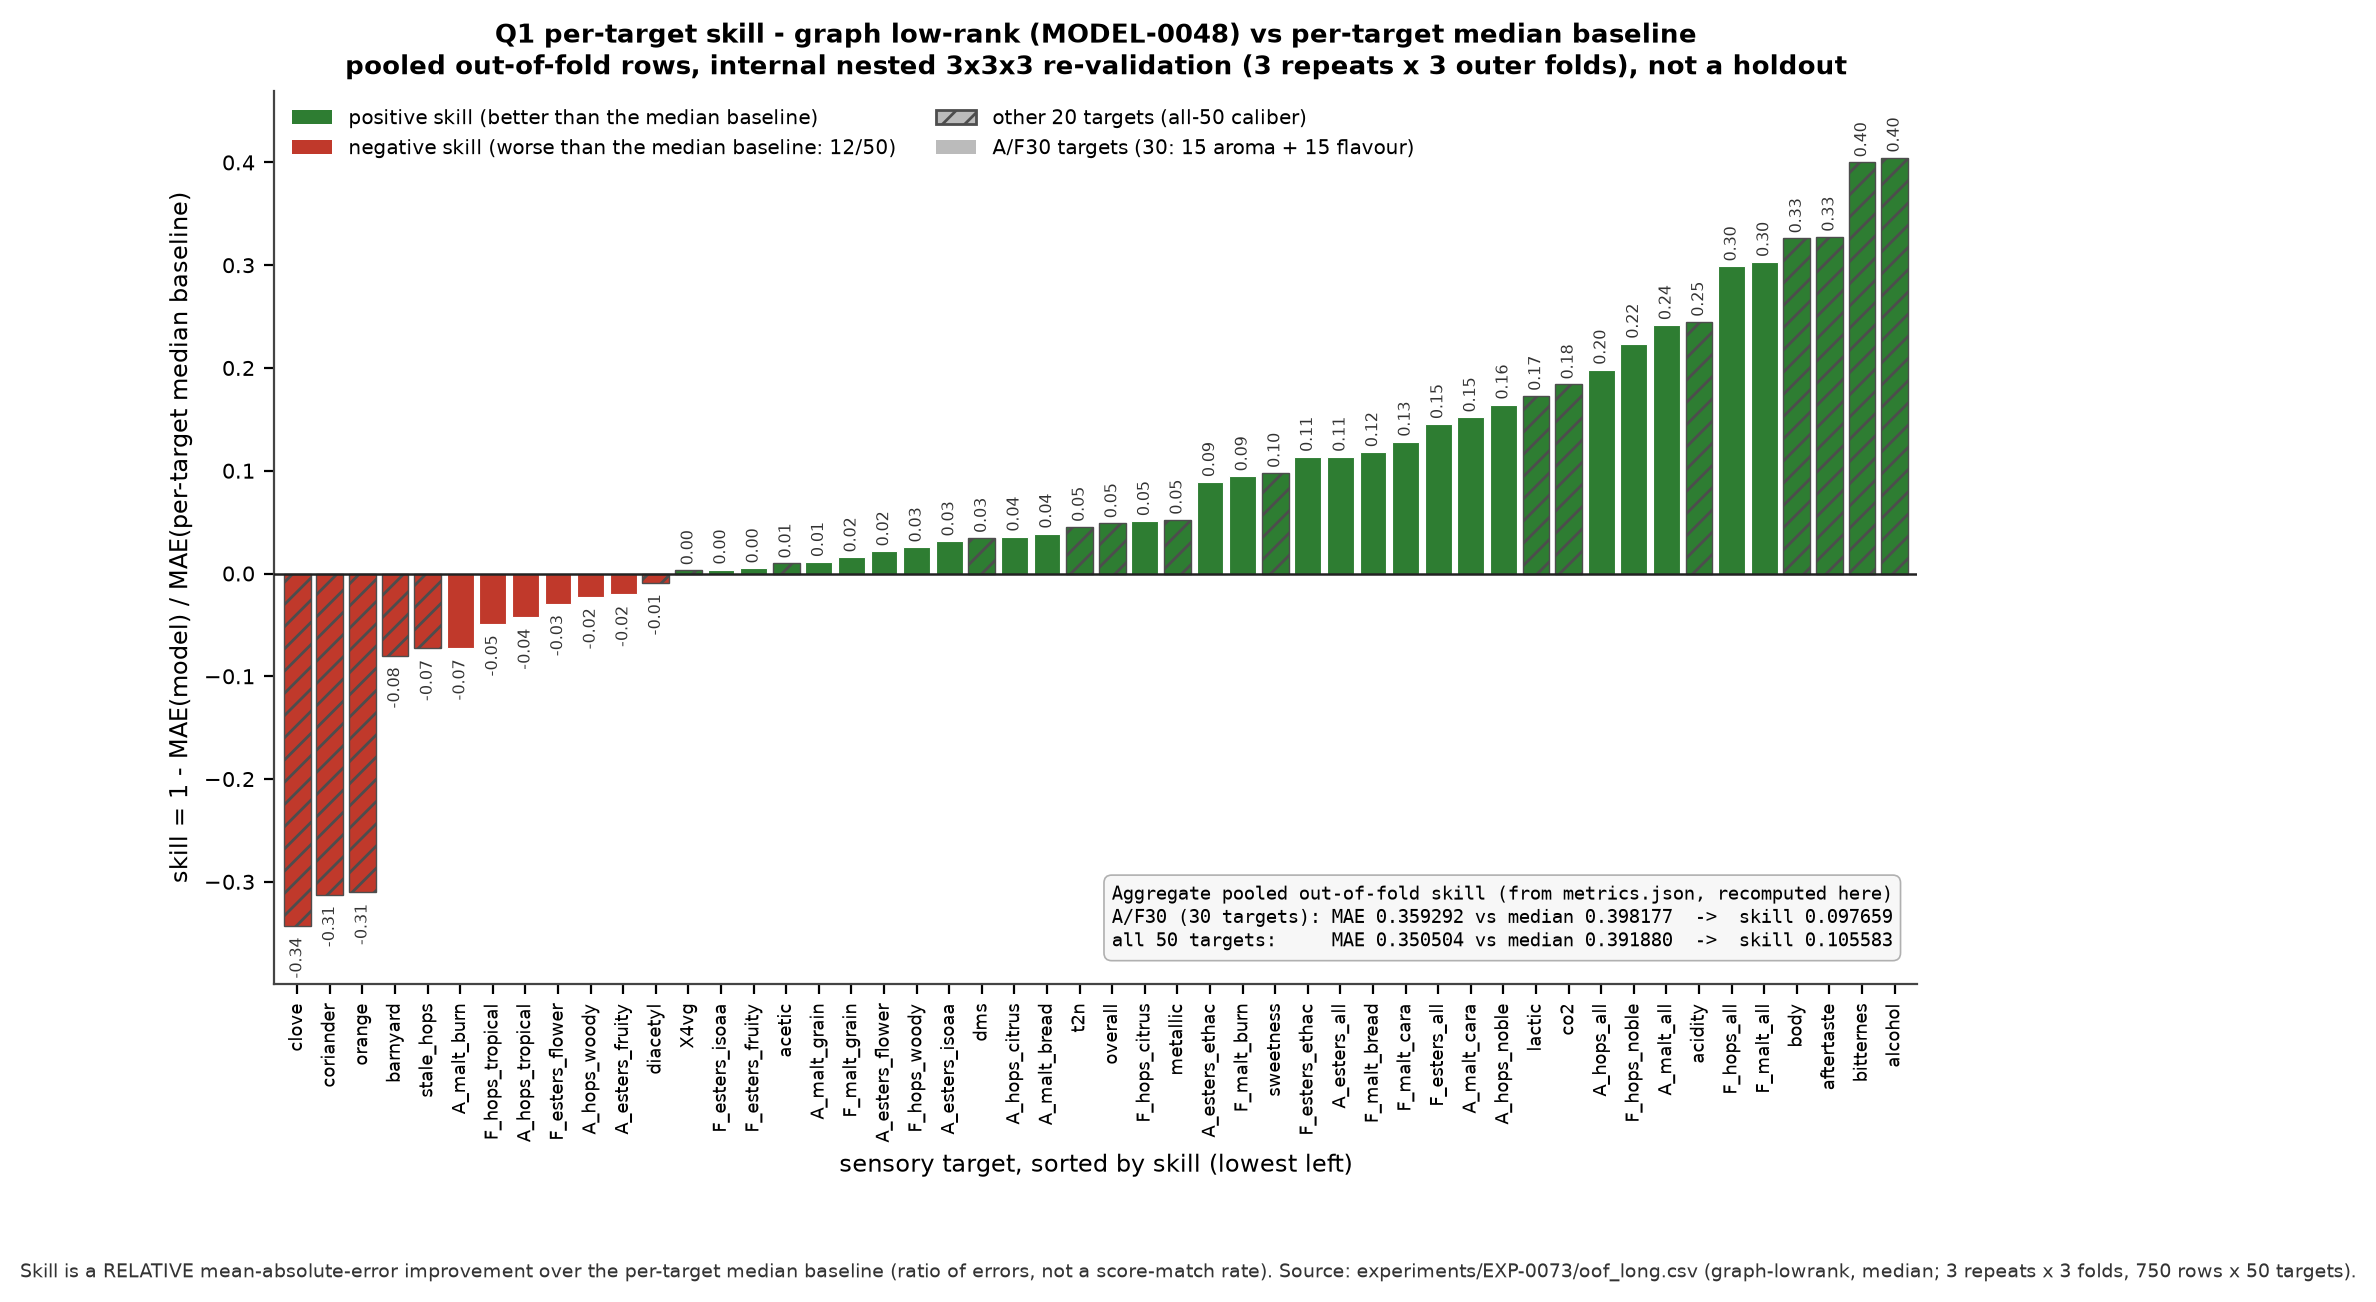
\includegraphics[width=0.92\linewidth,height=0.42\textheight,keepaspectratio]{../figures/confirmatory/Q1-per-target-skill.png}
\captionof{figure}{问题一：逐目标相对误差改善 1−MAE模型/MAE中位数（图低秩，内部嵌套CV折外池化）；A/F30 0.0977、全50维 0.1056，12 个目标为负。（\texttt{FIG-0032}）}
\end{bpfigure}

\begin{bpfigure}
%% figure-id: FIG-0033 sha256:a461da972ec8e999b9d643e945cf792f262d61c88aa85680fc67e7ba8119122e
%% figure-src: ../figures/confirmatory/Q1-model-comparison.png
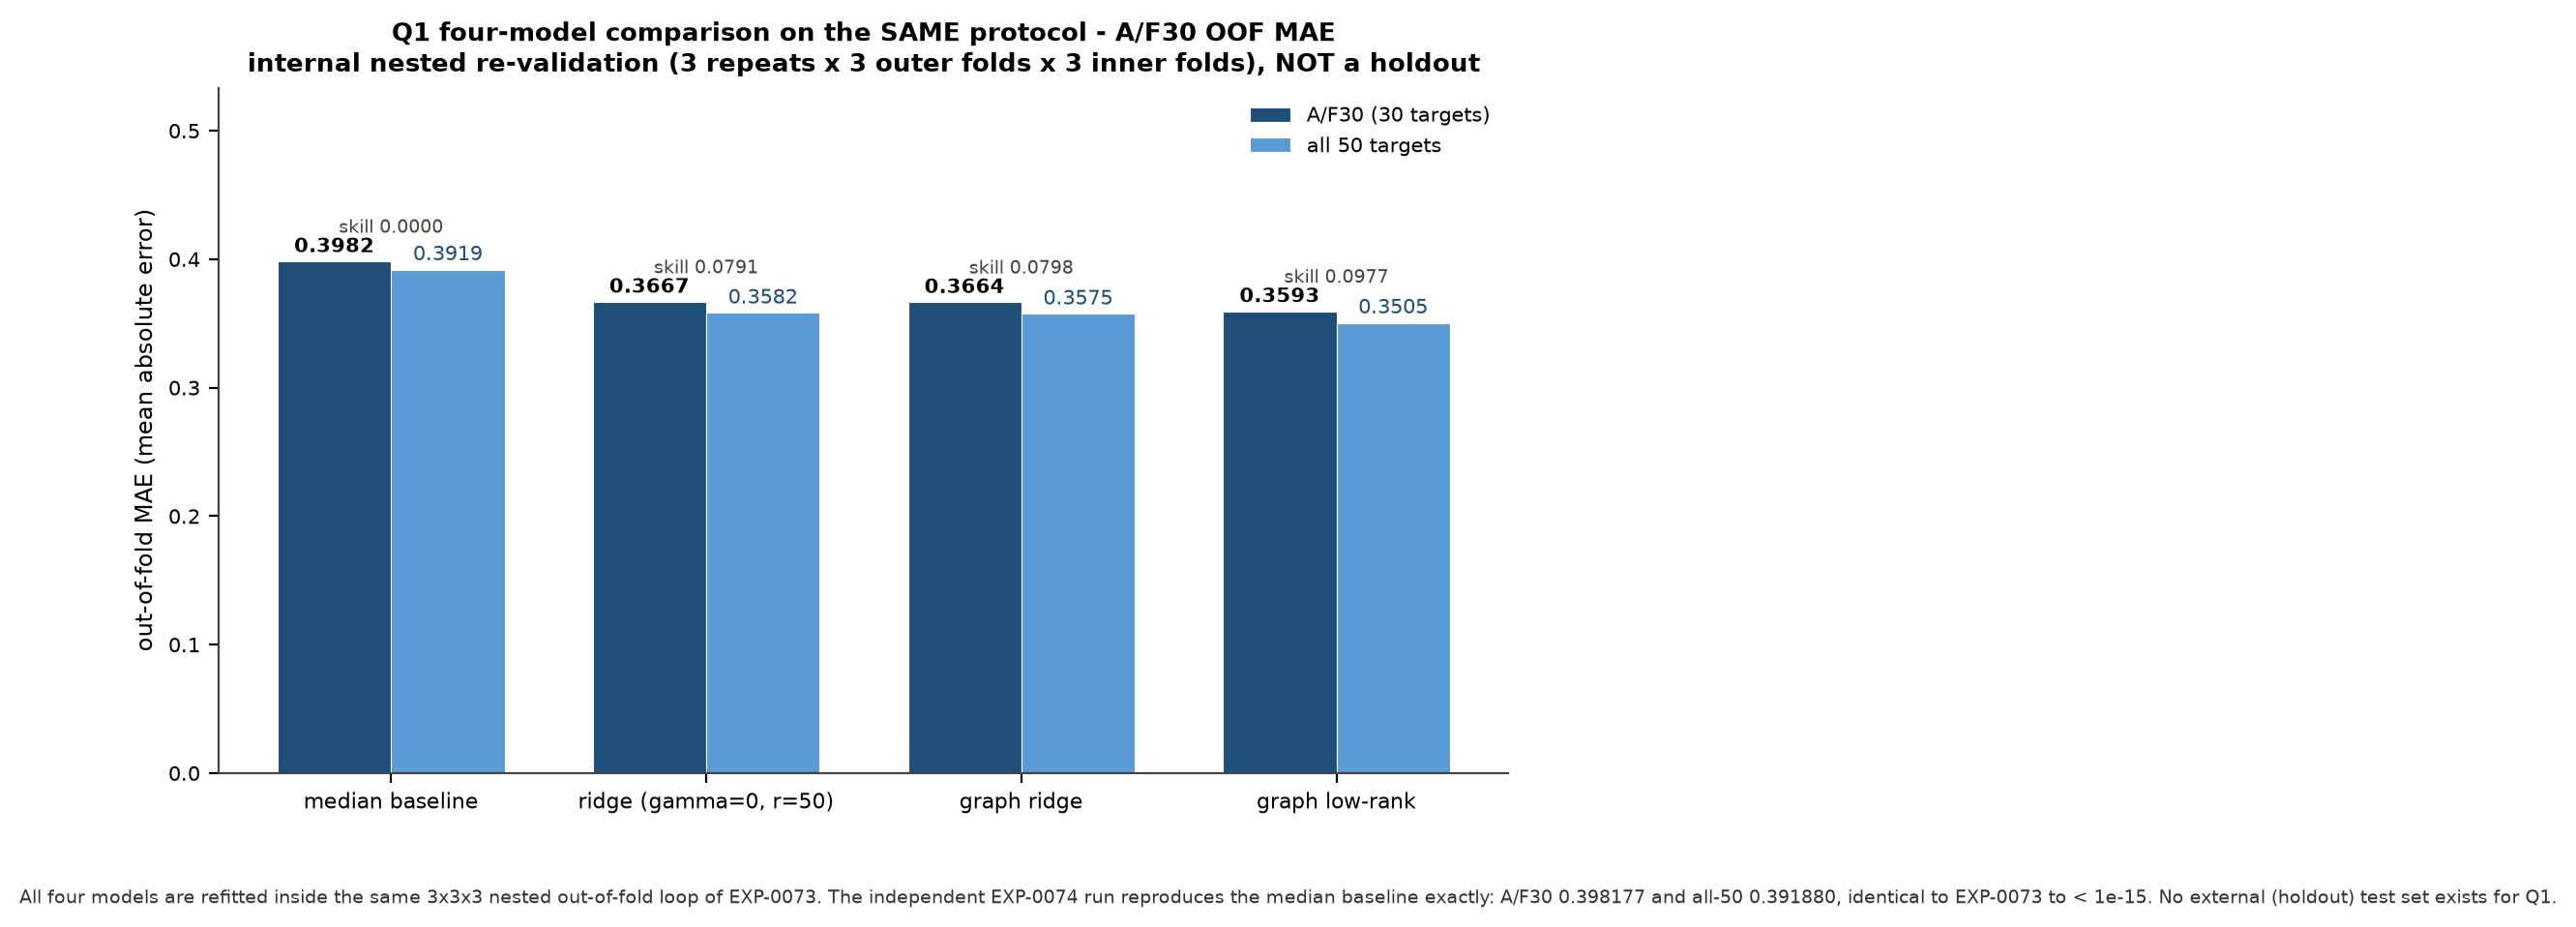
\includegraphics[width=0.92\linewidth,height=0.42\textheight,keepaspectratio]{../figures/confirmatory/Q1-model-comparison.png}
\captionof{figure}{问题一：四模型同协议折外MAE（内部3×3×3嵌套重验证，非holdout）：中位数0.398、岭0.367、图岭0.366、图低秩0.359；全50维另列。（\texttt{FIG-0033}）}
\end{bpfigure}

值得注意的是两个\textbf{负结果}。第一，普通 Ridge 的 30 维 MAE 为
0.3666617580105253，图 Ridge 为
0.3664110157826924，两者差异远小于它们与中位数基线的差距：在本协议下，仅加入图正则几乎不改变误差，图结构的收益只在叠加低秩约束后才出现。第二，图低秩模型相对普通
Ridge 的改善同样不大：请对照表 q1-models 中``普通
Ridge''与``图正则低秩''两行，两者的差距小于它们与中位数基线的差距。因此本文把图与低秩组件的作用定位为``提供多输出共享结构与可解释系数''，而不是``带来稳定领先的预测增益''。这与逐折波动的量级一致：9
个折的 MAE 并不落在同一水平上，组间与折间差异见下表。

\begin{bptable}
\setcounter{table}{1}
%% table-id: q1-groups sha256:346c55460e3fde077cdaf481cd0930060902cd08f0cf121bed75678c70c8228a
\captionof{table}{指标分组误差与折间波动}\label{tab:q1-groups}
\par\smallskip
\small
\begin{tabular}{@{}llrrr@{}}
\toprule
对象 & 口径 & MAE & 样本数 & 同折中位数基线 MAE \\
\midrule
香气 15 维（指标组） & 指标组 & 0.3646 & 15 & — \\
风味 15 维（指标组） & 指标组 & 0.3540 & 15 & — \\
其余 20 维（指标组） & 指标组 & 0.3373 & 20 & — \\
第 1 次重复 ·\allowbreak{} 第 1 折 & 折外分段 & 0.3549 & 91 & 0.4024 \\
第 1 次重复 ·\allowbreak{} 第 2 折 & 折外分段 & 0.3450 & 83 & 0.3794 \\
第 1 次重复 ·\allowbreak{} 第 3 折 & 折外分段 & 0.3635 & 76 & 0.4124 \\
第 2 次重复 ·\allowbreak{} 第 1 折 & 折外分段 & 0.3643 & 76 & 0.4039 \\
第 2 次重复 ·\allowbreak{} 第 2 折 & 折外分段 & 0.3618 & 91 & 0.3882 \\
第 2 次重复 ·\allowbreak{} 第 3 折 & 折外分段 & 0.3614 & 83 & 0.4044 \\
第 3 次重复 ·\allowbreak{} 第 1 折 & 折外分段 & 0.3492 & 83 & 0.3771 \\
第 3 次重复 ·\allowbreak{} 第 2 折 & 折外分段 & 0.3731 & 76 & 0.4165 \\
第 3 次重复 ·\allowbreak{} 第 3 折 & 折外分段 & 0.3623 & 91 & 0.4026 \\
\bottomrule
\end{tabular}
\begin{tablenote}注：上三行为三个指标组的折外池化 MAE 与组内维数；下九行为三次重复 × 三次外折逐折的折外 MAE、折内行数与同一折的中位数基线 MAE，用于展示折间波动而非模型间比较。逐折行数不同是因为外折按风格分层切分。\end{tablenote}
\end{bptable}

分组的结论是方向性的而非量级性的：口感、缺陷与总体评价构成的 20
维组，其误差低于 Aroma 与 Flavour 两个 15 维组；Aroma
组最高。逐风格结果（附录表
q1-styles）进一步显示，样本量很小的风格误差明显更大，且同一模型在不同风格上的排序并不稳定，这与其训练行数直接相关。

逐维结果见附录表 q1-targets，按 Skill 升序排列以暴露恶化维度：总体 Skill
为正并不意味着每一维都改善，把汇总值当作逐维结论是本协议下最常见的误读。

\subsection{0--6
相对等级与典型评分表}\label{ux76f8ux5bf9ux7b49ux7ea7ux4e0eux5178ux578bux8bc4ux5206ux8868}

由于附件未提供原始整数评分及其标准化参数，本文定义可复核的相对强度等级。以该目标外层训练标签的中点经验分布函数
\(\widehat F_t^{\mathrm{mid}}\) 标定：

\[\bpMathFit{
a_{it}=\widehat F_t^{\mathrm{mid}}(\widehat y_{it}),\qquad
g_{it}^{\mathrm{cont}}=6a_{it},\qquad
g_{it}=\min\{6,\max[0,\lfloor 6a_{it}+1/2\rfloor]\}.
}\]

对观测侧使用\textbf{同一个}
\(\widehat F_t^{\mathrm{mid}}\)，因此两侧处于同一标尺，可比较的只有``相对等级一致性''，不是与原始人工评分的一致性。预测落在训练分布中位附近时等级约为
3，靠近两端时趋向 0 或 6。0 不表示该风味不存在，6
不表示恢复了人工满分，缺陷维度的高等级也不等于超出物理阈值。

\begin{bptable}
\setcounter{table}{2}
%% table-id: q1-grades sha256:003871a907665e16bf0094c63cb04e80637c3fb52cff89ac95e07d60eb05f214
\captionof{table}{各模型的相对等级一致性}\label{tab:q1-grades}
\par\smallskip
\small
\begin{tabular}{@{}>{\raggedright\arraybackslash}p{\dimexpr 0.2185\linewidth-6pt\relax}>{\raggedleft\arraybackslash}p{\dimexpr 0.0855\linewidth-6pt\relax}>{\raggedleft\arraybackslash}p{\dimexpr 0.0987\linewidth-6pt\relax}>{\raggedleft\arraybackslash}p{\dimexpr 0.0993\linewidth-6pt\relax}>{\raggedleft\arraybackslash}p{\dimexpr 0.0634\linewidth-6pt\relax}>{\raggedleft\arraybackslash}p{\dimexpr 0.0634\linewidth-6pt\relax}>{\raggedleft\arraybackslash}p{\dimexpr 0.0634\linewidth-6pt\relax}>{\raggedleft\arraybackslash}p{\dimexpr 0.0745\linewidth-6pt\relax}>{\raggedleft\arraybackslash}p{\dimexpr 0.0745\linewidth-6pt\relax}>{\raggedleft\arraybackslash}p{\dimexpr 0.0634\linewidth-6pt\relax}>{\raggedleft\arraybackslash}p{\dimexpr 0.0634\linewidth-6pt\relax}@{}}
\toprule
模型 & 等级 MAE & 整级一致率 & 二次加权 κ & 等级 0 & 等级 1 & 等级 2 & 等级 3 & 等级 4 & 等级 5 & 等级 6 \\
\midrule
图正则低秩 & 1.4111 & 0.2289 & 0.3321 & 1315 & 1915 & 4151 & 9493 & 13092 & 7140 & 394 \\
图 Ridge & 1.4391 & 0.2150 & 0.2590 & 412 & 1007 & 3156 & 11488 & 15347 & 5985 & 105 \\
普通 Ridge & 1.4401 & 0.2105 & 0.2390 & 141 & 699 & 2787 & 12102 & 16372 & 5388 & 11 \\
最小中位数基线 & 1.5072 & 0.1650 & 0.0000 & 0 & 0 & 0 & 37500 & 0 & 0 & 0 \\
参照等级（真实标签同映射） & — & — & — & 3190 & 6229 & 6227 & 6189 & 6259 & 6211 & 3195 \\
\bottomrule
\end{tabular}
\begin{tablenote}注：等级为训练折内经验中点分布映射出的 0–6 相对强度等级，参照等级是真实标准化标签经同一映射得到的等级；本表衡量的是相对等级的一致性，不是恢复人工感官评分，也不代表等级 0/6 对应原始评分卡的 0/6 分。二次加权 κ 与整级一致率均在 37500 个等级格（750 行 × 50 维）上计算；最小中位数基线的预测恒为中间等级，其等级分布只有一档，因此 κ 为 0。预测等级向中间收缩，说明离散等级仍有改善空间。\end{tablenote}
\end{bptable}

回归预测向中部收缩，使预测等级分布集中在中间等级，而参照等级在 0--6
上接近均匀；两者的整级一致率、二次加权 \(\kappa\) 与等级 MAE
因此受限（表 q1-grades）。这是本方法的真实短板，不作为可忽略的枝节。

\begin{bpfigure}
%% figure-id: FIG-0034 sha256:e2cf95cdb0e4fa5d16a79db21f08f1abc8f8136346a2b02612285ea60daa27d4
%% figure-src: ../figures/confirmatory/Q1-grade-distribution.png
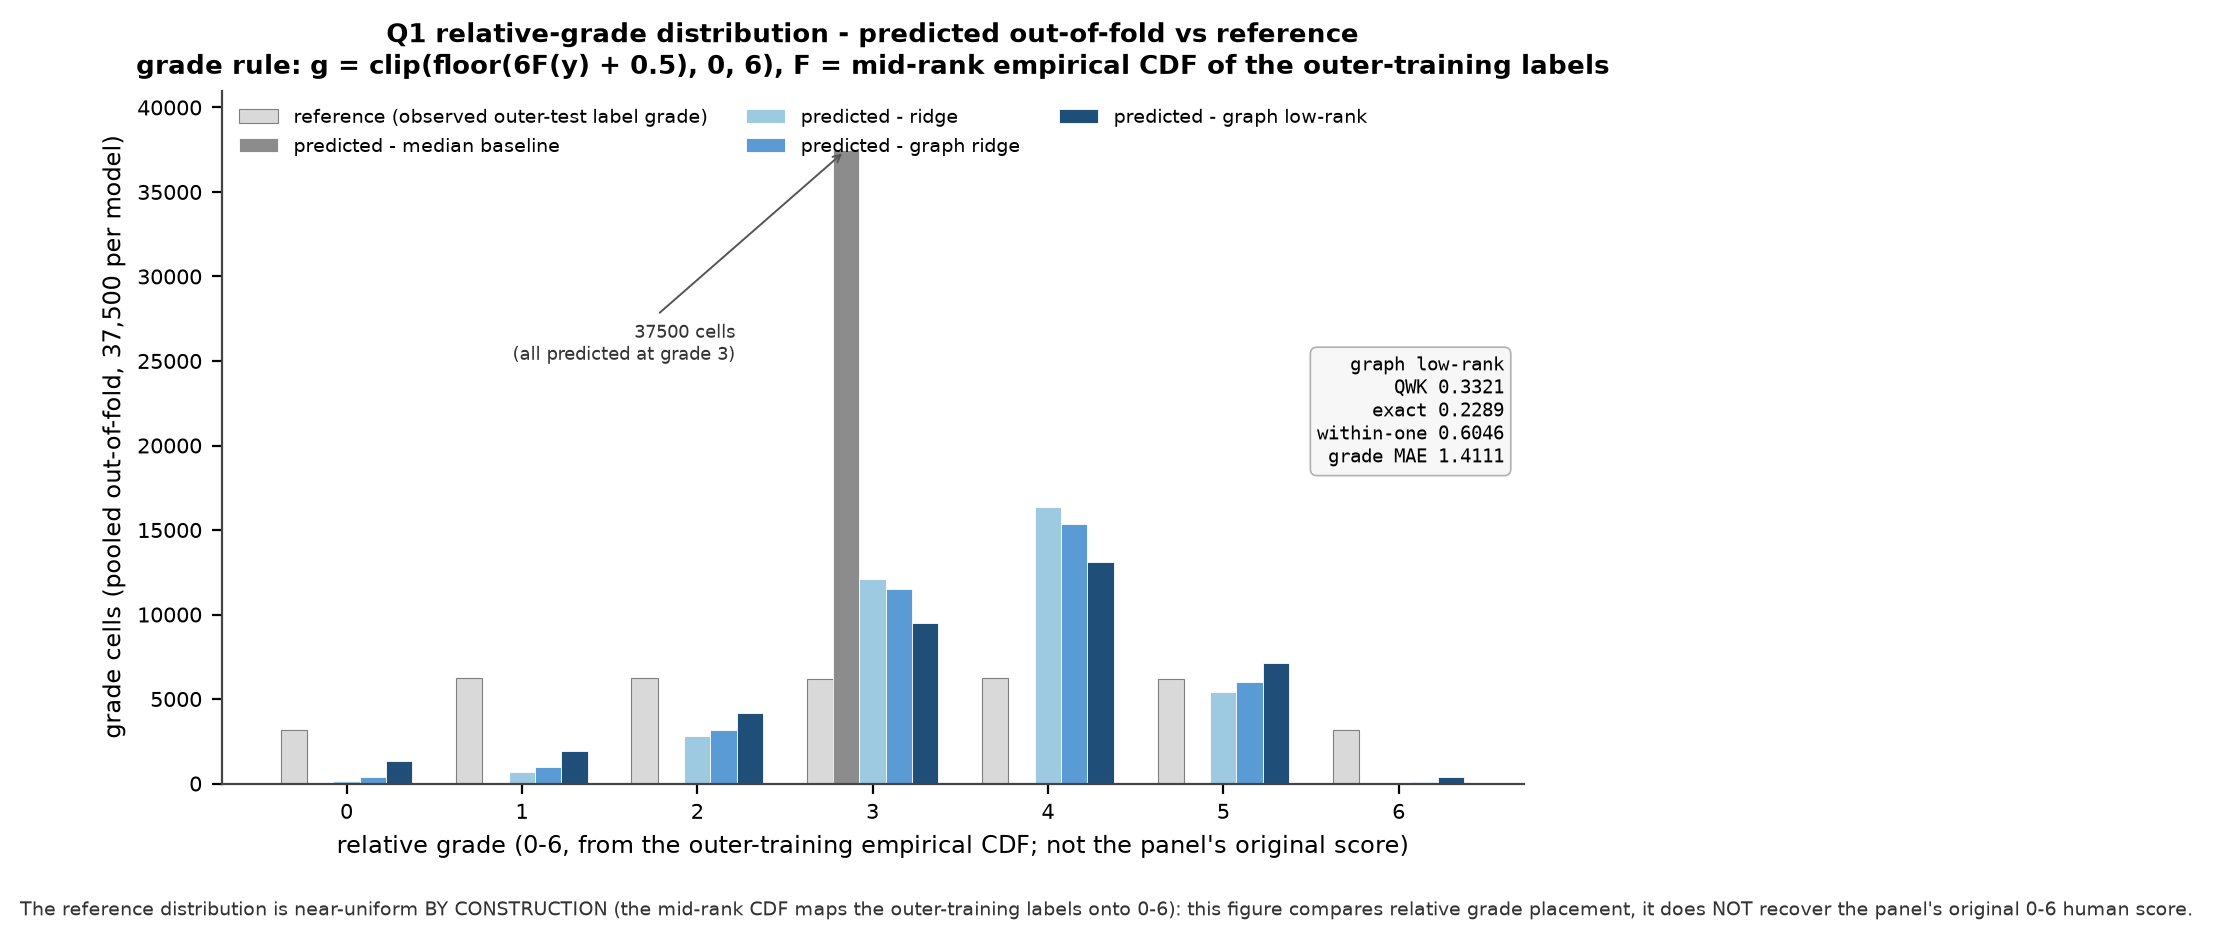
\includegraphics[width=0.92\linewidth,height=0.42\textheight,keepaspectratio]{../figures/confirmatory/Q1-grade-distribution.png}
\captionof{figure}{问题一：相对等级 0–6 的折外预测分布与参照分布对照（内部嵌套CV、中秩经验CDF；属相对等级，未恢复人工评分）。（\texttt{FIG-0034}）}
\end{bpfigure}

表 q1-scores-aroma、q1-scores-flavour 依据 \texttt{beer} 的真实序号提取
Beer\#1--Beer\#10，与评分卡中的 Beer\#
对齐，列出核心维度的相对等级；全部 250 款啤酒 × 50
维的连续预测与整数分级随支撑材料提供，表中只截取核心维度。

\begin{bptable}
\setcounter{table}{3}
%% table-id: q1-scores-aroma sha256:0040ad38b0b93fa8a8f0ee6935edc3ad3d1da2916f6b9db8d38f360b526ba4d1
\captionof{table}{Beer\#1–Beer\#10 的 Aroma 核心维度相对等级}\label{tab:q1-scores-aroma}
\par\smallskip
\small
\begin{tabular}{@{}>{\raggedright\arraybackslash}p{\dimexpr 0.0966\linewidth-6pt\relax}>{\raggedleft\arraybackslash}p{\dimexpr 0.0890\linewidth-6pt\relax}>{\raggedleft\arraybackslash}p{\dimexpr 0.0890\linewidth-6pt\relax}>{\raggedleft\arraybackslash}p{\dimexpr 0.0707\linewidth-6pt\relax}>{\raggedleft\arraybackslash}p{\dimexpr 0.0890\linewidth-6pt\relax}>{\raggedleft\arraybackslash}p{\dimexpr 0.0981\linewidth-6pt\relax}>{\raggedleft\arraybackslash}p{\dimexpr 0.0890\linewidth-6pt\relax}>{\raggedleft\arraybackslash}p{\dimexpr 0.0890\linewidth-6pt\relax}>{\raggedleft\arraybackslash}p{\dimexpr 0.0707\linewidth-6pt\relax}>{\raggedleft\arraybackslash}p{\dimexpr 0.0890\linewidth-6pt\relax}>{\raggedleft\arraybackslash}p{\dimexpr 0.0981\linewidth-6pt\relax}@{}}
\toprule
样本 & 香气·\allowbreak{}麦芽总体·\allowbreak{}预测 & 香气·\allowbreak{}酒花总体·\allowbreak{}预测 & 香气·\allowbreak{}柑橘·\allowbreak{}预测 & 香气·\allowbreak{}酯香总体·\allowbreak{}预测 & 香气·\allowbreak{}乙酸异戊酯·\allowbreak{}预测 & 香气·\allowbreak{}麦芽总体·\allowbreak{}参照 & 香气·\allowbreak{}酒花总体·\allowbreak{}参照 & 香气·\allowbreak{}柑橘·\allowbreak{}参照 & 香气·\allowbreak{}酯香总体·\allowbreak{}参照 & 香气·\allowbreak{}乙酸异戊酯·\allowbreak{}参照 \\
\midrule
Beer\#1 & 4 & 3 & 3 & 4 & 3 & 5 & 5 & 1 & 2 & 3 \\
Beer\#2 & 3 & 1 & 2 & 1 & 4 & 3 & 0 & 0 & 0 & 0 \\
Beer\#3 & 3 & 2 & 3 & 4 & 4 & 2 & 2 & 4 & 4 & 4 \\
Beer\#4 & 4 & 3 & 4 & 4 & 4 & 4 & 3 & 4 & 5 & 3 \\
Beer\#5 & 1 & 5 & 5 & 3 & 3 & 5 & 5 & 6 & 4 & 5 \\
Beer\#6 & 4 & 3 & 3 & 4 & 4 & 1 & 1 & 4 & 5 & 5 \\
Beer\#7 & 1 & 5 & 5 & 4 & 3 & 1 & 6 & 6 & 1 & 2 \\
Beer\#8 & 3 & 5 & 4 & 4 & 4 & 4 & 6 & 5 & 4 & 4 \\
Beer\#9 & 3 & 5 & 4 & 3 & 3 & 3 & 5 & 5 & 3 & 4 \\
Beer\#10 & 1 & 1 & 4 & 1 & 2 & 1 & 3 & 6 & 5 & 5 \\
\bottomrule
\end{tabular}
\begin{tablenote}注：等级为训练折内经验分布映射得到的 0–6 相对强度等级，预测列为折外预测、参照列为真实标签经同一映射的等级；样本编号与题面评分卡的 Beer\# 对齐（第 n 号样本即 beer\_n 评分卡对应的啤酒）；表内为首轮重复的折外结果，五维为核心香气维度（麦芽总体、酒花总体、柑橘、酯香总体、乙酸异戊酯）；等级是相对强度，不是人工评分恢复，也不表示风味存在与否。\end{tablenote}
\end{bptable}

\begin{bptable}
\setcounter{table}{4}
%% table-id: q1-scores-flavour sha256:a1ab3464521df13d9e0f039f6bdaf35522034adc6015fb6022fbdd8830359165
\captionof{table}{Beer\#1–Beer\#10 的 Flavour 核心维度相对等级}\label{tab:q1-scores-flavour}
\par\smallskip
\small
\begin{tabular}{@{}>{\raggedright\arraybackslash}p{\dimexpr 0.0966\linewidth-6pt\relax}>{\raggedleft\arraybackslash}p{\dimexpr 0.0890\linewidth-6pt\relax}>{\raggedleft\arraybackslash}p{\dimexpr 0.0890\linewidth-6pt\relax}>{\raggedleft\arraybackslash}p{\dimexpr 0.0707\linewidth-6pt\relax}>{\raggedleft\arraybackslash}p{\dimexpr 0.0890\linewidth-6pt\relax}>{\raggedleft\arraybackslash}p{\dimexpr 0.0981\linewidth-6pt\relax}>{\raggedleft\arraybackslash}p{\dimexpr 0.0890\linewidth-6pt\relax}>{\raggedleft\arraybackslash}p{\dimexpr 0.0890\linewidth-6pt\relax}>{\raggedleft\arraybackslash}p{\dimexpr 0.0707\linewidth-6pt\relax}>{\raggedleft\arraybackslash}p{\dimexpr 0.0890\linewidth-6pt\relax}>{\raggedleft\arraybackslash}p{\dimexpr 0.0981\linewidth-6pt\relax}@{}}
\toprule
样本 & 风味·\allowbreak{}麦芽总体·\allowbreak{}预测 & 风味·\allowbreak{}酒花总体·\allowbreak{}预测 & 风味·\allowbreak{}柑橘·\allowbreak{}预测 & 风味·\allowbreak{}酯香总体·\allowbreak{}预测 & 风味·\allowbreak{}乙酸异戊酯·\allowbreak{}预测 & 风味·\allowbreak{}麦芽总体·\allowbreak{}参照 & 风味·\allowbreak{}酒花总体·\allowbreak{}参照 & 风味·\allowbreak{}柑橘·\allowbreak{}参照 & 风味·\allowbreak{}酯香总体·\allowbreak{}参照 & 风味·\allowbreak{}乙酸异戊酯·\allowbreak{}参照 \\
\midrule
Beer\#1 & 3 & 3 & 3 & 4 & 3 & 5 & 4 & 1 & 5 & 6 \\
Beer\#2 & 3 & 1 & 2 & 1 & 4 & 4 & 0 & 3 & 0 & 0 \\
Beer\#3 & 3 & 2 & 3 & 4 & 4 & 2 & 2 & 4 & 3 & 5 \\
Beer\#4 & 4 & 3 & 3 & 4 & 4 & 5 & 4 & 3 & 6 & 4 \\
Beer\#5 & 2 & 5 & 5 & 2 & 3 & 5 & 6 & 4 & 4 & 3 \\
Beer\#6 & 4 & 3 & 3 & 4 & 4 & 2 & 2 & 4 & 4 & 4 \\
Beer\#7 & 2 & 5 & 5 & 4 & 4 & 2 & 6 & 5 & 3 & 1 \\
Beer\#8 & 4 & 5 & 4 & 4 & 4 & 2 & 6 & 4 & 6 & 4 \\
Beer\#9 & 4 & 5 & 4 & 3 & 3 & 3 & 5 & 6 & 3 & 1 \\
Beer\#10 & 0 & 0 & 4 & 1 & 3 & 0 & 3 & 6 & 6 & 6 \\
\bottomrule
\end{tabular}
\begin{tablenote}注：等级为训练折内经验分布映射得到的 0–6 相对强度等级，预测列为折外预测、参照列为真实标签经同一映射的等级；样本编号与题面评分卡的 Beer\# 对齐（第 n 号样本即 beer\_n 评分卡对应的啤酒）；表内为首轮重复的折外结果，五维为核心风味维度（麦芽总体、酒花总体、柑橘、酯香总体、乙酸异戊酯）；等级是相对强度，不是人工评分恢复，也不表示风味存在与否。\end{tablenote}
\end{bptable}

样本间差异已经体现在整数等级中：同一维度在不同酒款上跨越多个等级，说明该维度在本数据内可分；但相邻等级之间没有可核对的原始评分作为标尺，等级差
1 不应读作``强度差 1 个单位''。

\subsection{问题一的作用边界}\label{ux95eeux9898ux4e00ux7684ux4f5cux7528ux8fb9ux754c}

问题一的结果有四条硬边界，必须与数值同时阅读。

第一，没有留出集。全样本 3×3×3
嵌套交叉验证的每一行预测都是折外预测，但不存在一个从未参与任何拟合的外部样本集。``留出泛化''与``外部验证''类陈述在本问中不成立；本问能支持的最强陈述是``在冻结协议下的内部折外重验证''。

第二，划分完整性检查结构性不可满足。评价实验没有登记数据划分，工具对划分完整性检查给出具名拒绝；同理，由于不存在留出集，留出指标检查也不可满足。这两项不是遗漏，而是协议选择的结果，本文如实披露而不通过另挂旧划分来规避。相应地，本问的选择状态只到草稿选择，不放行为已验证。

第三，固定种子的独立复跑只证明确定性重现。复跑实验与外层实验逐位一致，说明代码与数据在同一环境下的可重复性，但它不引入新样本、也不是独立实现，不能作为泛化证据。稳健性检验只覆盖三个冻结种子中的两个，见后文限制一节。

第四，结论只适用于当前冻结候选（图正则低秩）、当前数据版本与当前协议。更换候选、更换数据或改变划分/协议后，本节的误差与等级数字都不可沿用；本文没有对``其他候选是否同样适用''做任何检验。

\textbf{证据登记（问题一稳健性）。}
问题一的稳健性检验同时覆盖种子扰动与内层正则强度扰动：Aroma/Flavour 30
维等权 MAE 分别为 0.3542、0.3624、0.3576，绝对极差 0.0082、相对极差
0.0232，均在预设上限 0.05
之内。该检验只覆盖三个冻结种子中的两个，扰动也只沿单一参数方向（内层正则网格整体乘
0.5）；固定种子的独立复跑只证明确定性重现，不构成独立实现或独立稳健性证据。

\section{问题二：共表达网络、风格混杂与稳定
Top-3}\label{ux95eeux9898ux4e8cux5171ux8868ux8fbeux7f51ux7edcux98ceux683cux6df7ux6742ux4e0eux7a33ux5b9a-top-3}

\subsection{候选宇宙：严格单体化合物与扩展指标分表}\label{ux5019ux9009ux5b87ux5b99ux4e25ux683cux5355ux4f53ux5316ux5408ux7269ux4e0eux6269ux5c55ux6307ux6807ux5206ux8868}

231
个化学及理化变量并非同一类对象。按化学语义拆分为四类：单体化合物、元素或成分指数、理化参数、派生汇总。严格单体化合物构成
216 项，是``关键化合物因素''的主表候选；元素与成分指数 3 项、理化参数 7
项、派生汇总 5 项共 15
项构成扩展表。原先被标为单体的铁含量、蛋白质总量与
\(\beta\)-葡聚糖三项在本轮被重新归类为元素或成分指数，不再进入严格表。

\begin{bptable}
\setcounter{table}{5}
%% table-id: q2-universe sha256:83af9df245dda67a83065e9a76f2423297dfaf46130b6480ca401951ef8b69bd
\captionof{table}{候选宇宙构成与两张表的划分}\label{tab:q2-universe}
\par\smallskip
\small
\begin{tabular}{@{}>{\raggedright\arraybackslash}p{\dimexpr 0.1222\linewidth-6pt\relax}>{\raggedleft\arraybackslash}p{\dimexpr 0.0745\linewidth-6pt\relax}>{\raggedright\arraybackslash}p{\dimexpr 0.1222\linewidth-6pt\relax}>{\raggedright\arraybackslash}p{\dimexpr 0.1222\linewidth-6pt\relax}>{\raggedright\arraybackslash}p{\dimexpr 0.5267\linewidth-6pt\relax}@{}}
\toprule
类别 & 候选数 & 进入严格榜 & 进入扩展榜 & 说明 \\
\midrule
单体化合物 & 216 & 是 & 否 & 严格榜唯一允许的宇宙：参与 50 维 Top-3 选择 \\
元素/\allowbreak{}指数 & 3 & 否 & 是 & 元素/\allowbreak{}指数项，非单体化合物，移出严格榜 \\
理化参数 & 7 & 否 & 是 & 理化参数，非化合物丰度，只进扩展榜 \\
派生和 & 5 & 否 & 是 & 派生汇总量，不是独立化合物，只进扩展榜 \\
合计 & 231 & — & — & 候选矩阵为 231 个候选 × 50 个维度 \\
\bottomrule
\end{tabular}
\begin{tablenote}注：严格榜只允许单体化合物，元素/指数、理化参数与派生和另一张扩展榜单独报告，两张表不得混排；同一化合物在不同维度上的候选一致。候选矩阵共 231 个候选 × 50 个维度 = 11550 个候选-维度单元。\end{tablenote}
\end{bptable}

分表不是形式主义：把蛋白质总量、铁含量与``热量''一类的汇总量与挥发性风味分子混在同一张
Top-3
表里，会让``关键化合物''的语义失效。因此正文的核心表只含严格单体化合物，扩展表单独给出，两者不合并统计。

\subsection{两个用途不同的网络}\label{ux4e24ux4e2aux7528ux9014ux4e0dux540cux7684ux7f51ux7edc}

附件相关矩阵用于描述全部样本中的化合物协同变化，其边权按
\(|\rho|\ge\tau\)
取阈值；由于该矩阵不保证严格半正定，构图前先作半正定投影，再把投影后的矩阵作为描述性网络的权重来源。预测与关联模型使用的图则是每次由当前训练行重新估计的：中位数填补后的
231 列计算中秩 Spearman，取
\(w_{jk}=\widehat\rho_{jk}\mathbf1\{|\widehat\rho_{jk}|\ge\tau\}\)，\(\tau=0.5\)
冻结，对角置零。

两类网络的统计量不可混用：描述网络回答``这批样本里谁与谁共同变化''，训练网络只承担正则化与结构化系数提取。连通分量表示阈值图上的传递连通，并不等同于经过功能验证的生物化学模块，因此模块标签不进入
Top-3 综合打分。

\textbf{本轮实际重算并上图的是训练网络}：它由问题二注册的 200
行训练集按同一 \(\tau=0.5\)
规则重估，边数与分量数见图注。附件全样本相关矩阵（\texttt{2.csv}）已导入并登记
SHA，但其半正定投影阈值网络在本确认轮没有独立产物，因此本文不就该网络报告边数或分量数，也不得把它的统计量与训练网络混用。

\begin{bpfigure}
%% figure-id: FIG-0035 sha256:ad567a5eb75ba1b36012efc7d66b8d4e8e1667c348d2bf5cfa2f4f294410afc6
%% figure-src: ../figures/confirmatory/Q2-network.png
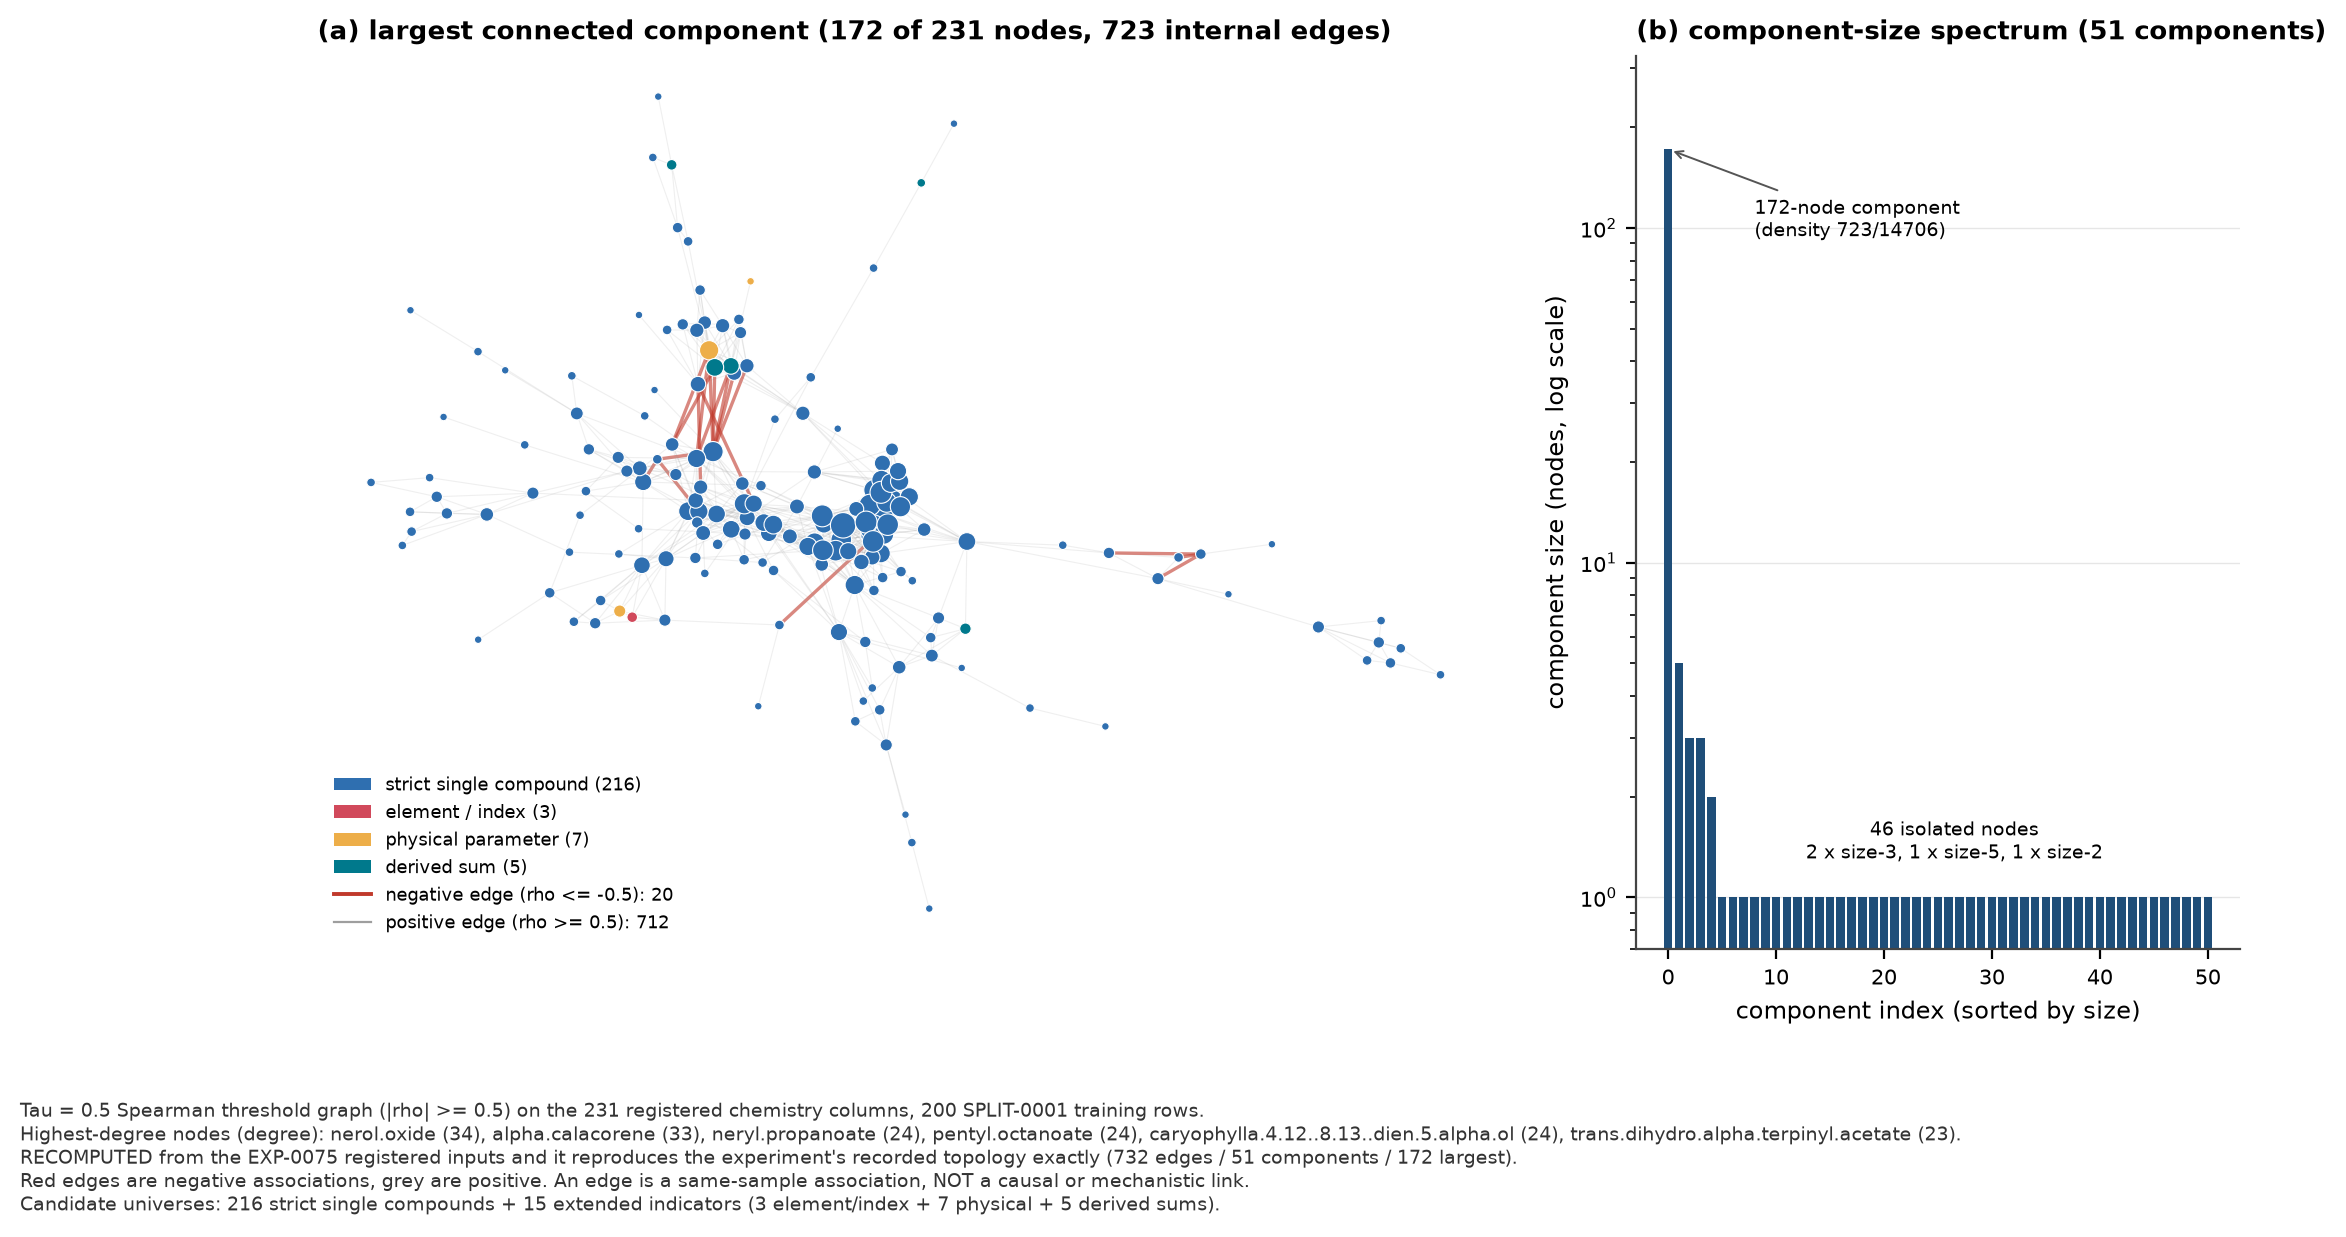
\includegraphics[width=0.92\linewidth,height=0.42\textheight,keepaspectratio]{../figures/confirmatory/Q2-network.png}
\captionof{figure}{问题二：τ=0.5 Spearman 阈值网络（由 EXP-0075 注册输入重算，复现 732 边/51 分量）；严格单体216与扩展15分色，边非因果。（\texttt{FIG-0035}）}
\end{bpfigure}

\subsection{风格混杂与残差化关联}\label{ux98ceux683cux6df7ux6742ux4e0eux6b8bux5deeux5316ux5173ux8054}

总体关联定义为
\(\rho^{\mathrm{total}}_{jt}=\operatorname{Spearman}(X_j,Y_t)\)。为分离组间风格差异，令
\(H\) 为风格虚拟变量与截距组成的设计矩阵，对秩残差化：

\[\bpMathFit{
P_H=H(H^\top H)^\dagger H^\top,\quad
r_j^X=(I-P_H)\operatorname{rank}(X_j),\quad
r_t^Y=(I-P_H)\operatorname{rank}(Y_t),\quad
\rho^{\mathrm{within}}_{jt}=\operatorname{Corr}(r_j^X,r_t^Y).
}\]

该指标反映去除风格均值差异后的共同关联。风格内残差化能减少组间差异的影响，但不能消除未观测混杂；因此本文同时保留总体关联，让两种口径并列，而不是用一种替换另一种。

\subsection{四种方法与综合打分}\label{ux56dbux79cdux65b9ux6cd5ux4e0eux7efcux5408ux6253ux5206}

对候选 \(j\) 与目标 \(t\) 使用四种方法：总体 Spearman、风格内残差化
Spearman、图低秩回归系数 \(\widehat B_{jt}\)、以及三者的共识分

\[\bpMathFit{
S_{jt}=\frac13\left[R\!\left(|\rho^{\mathrm{total}}_{jt}|\right)+R\!\left(|\rho^{\mathrm{within}}_{jt}|\right)+R\!\left(|\widehat B_{jt}|\right)\right],
}\]

其中 \(R\) 为同一目标内、该表自身候选宇宙上的百分位秩；\(\widehat B\)
来自固定 \(\tau=0.5,\ \lambda=1,\ \gamma=0.1,\ r=6\)
的图低秩模型。四种方法各自给出
Top-3，交付表使用共识分排序，方法间差异作为稳定性证据保留。

稳定性用风格分层 bootstrap 度量：在注册的 200 行训练集内，按
\texttt{tasting\_category\_fine}
分层、每层有放回重采样到自身规模，共重采样 500
次。每个重抽样样本都重新执行中位数填补、\(\tau=0.5\) 的 Spearman
图估计、图低秩回归、风格内秩残差化与三项子分数，然后重新取 Top-3：

\[\bpMathFit{
\pi_{jt}=\frac{1}{B}\sum_{b=1}^{B}\mathbf1\{j\in\operatorname{Top3}^{(b)}_t\},\qquad
\mathrm{se}_{\mathrm{mc}}=\sqrt{\frac{\pi_{jt}(1-\pi_{jt})}{B}} .
}\]

最终表按 \(\pi\) 降序排列，并列时按原样本综合分 \(S\)
裁决，再并列时沿用固定特征名的字符序。\(S\)
表征原样本中的综合关联强度，\(\pi\)
表征重抽样下的入选稳定性；候选方向取总体 Spearman
的符号，只是关联方向，不代表干预效应。每个入选条目旁同时报告同一参考模块内秩
4--10 的替代候选，使第三名的不稳定性不被隐藏。

\subsection{核心与完整
Top-3}\label{ux6838ux5fc3ux4e0eux5b8cux6574-top-3}

核心 20 个 Aroma/Flavour 维度的 Top-3 见表 q2-core-top3；完整 50
维、每维 3 项共 150 条目，以及 15 个扩展指标在 50 维上的
Top-3，均见支撑材料 \texttt{report/\allowbreak{}tables/\allowbreak{}q2-\allowbreak{}full-\allowbreak{}top3.md} 与
\texttt{report/\allowbreak{}tables/\allowbreak{}q2-\allowbreak{}extended.md}（同数据 CSV 与完整溯源在
\texttt{report/\allowbreak{}tables/\allowbreak{}INDEX.json}）。三张表的候选集合不同，不能相互替代或合并计数；移出正文只为篇幅，数据行未删减。

\begin{bpLTsmall}
\setcounter{table}{6}
\begin{longtable}{@{}>{\raggedright\arraybackslash}p{\dimexpr 0.0605\linewidth-6pt\relax}>{\raggedright\arraybackslash}p{\dimexpr 0.2264\linewidth-6pt\relax}>{\raggedright\arraybackslash}p{\dimexpr 0.2480\linewidth-6pt\relax}>{\raggedright\arraybackslash}p{\dimexpr 0.2369\linewidth-6pt\relax}>{\raggedright\arraybackslash}p{\dimexpr 0.1962\linewidth-6pt\relax}@{}}
%% table-id: q2-core-top3 sha256:b0b98a71dc2c4db096f7dbe7b88d35dfff710b2827a9da9869200ca293c03369
\caption{核心维度 Top-3 关键化学因素、入选频率与方向}\label{tab:q2-core-top3}\\
\toprule
感官维度 & 第 1 位 & 第 2 位 & 第 3 位 & 第 3 位同模块替代候选 \\
\midrule
\endfirsthead
\toprule
感官维度 & 第 1 位 & 第 2 位 & 第 3 位 & 第 3 位同模块替代候选 \\
\midrule
\endhead
\bottomrule
\endfoot
香气·\allowbreak{}麦芽总体 & furfural｜\allowbreak{}0.490/\allowbreak{}0.9767｜\allowbreak{}+·\allowbreak{}内 & X2.acetylfuran｜\allowbreak{}0.422/\allowbreak{}0.9597｜\allowbreak{}+·\allowbreak{}混 & beta.\allowbreak{}phellandrene｜\allowbreak{}0.340/\allowbreak{}0.9457｜\allowbreak{}−·\allowbreak{}混 & methylpyrazine \\
香气·\allowbreak{}谷物 & terpinen.4.ol｜\allowbreak{}0.296/\allowbreak{}0.9628｜\allowbreak{}−·\allowbreak{}混 & furfural｜\allowbreak{}0.252/\allowbreak{}0.9566｜\allowbreak{}+·\allowbreak{}混 & propylene.\allowbreak{}glycol｜\allowbreak{}0.200/\allowbreak{}0.9008｜\allowbreak{}−·\allowbreak{}内 & —（无） \\
香气·\allowbreak{}面包 & beta.\allowbreak{}phellandrene｜\allowbreak{}0.360/\allowbreak{}0.9581｜\allowbreak{}−·\allowbreak{}混 & X4.ethyl.\allowbreak{}guaiacol｜\allowbreak{}0.302/\allowbreak{}0.9457｜\allowbreak{}−·\allowbreak{}内 & furfural｜\allowbreak{}0.224/\allowbreak{}0.9287｜\allowbreak{}+·\allowbreak{}内 & —（无同模块替代） \\
香气·\allowbreak{}焦糖 & X2.methyl.\allowbreak{}benzofuran｜\allowbreak{}0.634/\allowbreak{}0.9674｜\allowbreak{}−·\allowbreak{}内 & furfural｜\allowbreak{}0.328/\allowbreak{}0.9674｜\allowbreak{}+·\allowbreak{}混 & X2.ethyl.1.hexanol｜\allowbreak{}0.238/\allowbreak{}0.8961｜\allowbreak{}−·\allowbreak{}混 & X2.acetylfuran \\
香气·\allowbreak{}烘烤 & ethyl.\allowbreak{}hydrocinnamate｜\allowbreak{}0.558/\allowbreak{}0.9860｜\allowbreak{}+·\allowbreak{}内 & selin.11.en.4.alpha.\allowbreak{}ol｜\allowbreak{}0.228/\allowbreak{}0.9380｜\allowbreak{}+·\allowbreak{}内 & SO2.mg.\allowbreak{}L.｜\allowbreak{}0.194/\allowbreak{}0.9287｜\allowbreak{}−·\allowbreak{}混 & —（无） \\
香气·\allowbreak{}酒花总体 & ethyl\_\allowbreak{}octanoate｜\allowbreak{}0.832/\allowbreak{}0.9829｜\allowbreak{}+·\allowbreak{}混 & cis.\allowbreak{}dihydro.\allowbreak{}beta.\allowbreak{}terpineol｜\allowbreak{}0.270/\allowbreak{}0.9271｜\allowbreak{}+·\allowbreak{}风 & DMS｜\allowbreak{}0.260/\allowbreak{}0.9209｜\allowbreak{}+·\allowbreak{}风 & —（无同模块替代） \\
香气·\allowbreak{}柑橘 & citronellol｜\allowbreak{}0.596/\allowbreak{}0.9674｜\allowbreak{}+·\allowbreak{}混 & geraniol｜\allowbreak{}0.502/\allowbreak{}0.9581｜\allowbreak{}+·\allowbreak{}混 & X1.alpha.\allowbreak{}terpineol｜\allowbreak{}0.238/\allowbreak{}0.9271｜\allowbreak{}+·\allowbreak{}内 & linalool \\
香气·\allowbreak{}热带水果 & beta.\allowbreak{}phellandrene｜\allowbreak{}0.666/\allowbreak{}0.9860｜\allowbreak{}+·\allowbreak{}内 & DMS｜\allowbreak{}0.648/\allowbreak{}0.9953｜\allowbreak{}+·\allowbreak{}混 & X.\allowbreak{}E..dihydro.\allowbreak{}apofarnesal｜\allowbreak{}0.202/\allowbreak{}0.9380｜\allowbreak{}−·\allowbreak{}混 & —（无） \\
香气·\allowbreak{}贵族酒花 & ethyl\_\allowbreak{}octanoate｜\allowbreak{}0.932/\allowbreak{}0.9953｜\allowbreak{}+·\allowbreak{}混 & ethyl\_\allowbreak{}decanoate｜\allowbreak{}0.692/\allowbreak{}0.9721｜\allowbreak{}+·\allowbreak{}混 & cis.\allowbreak{}dihydro.\allowbreak{}beta.\allowbreak{}terpineol｜\allowbreak{}0.200/\allowbreak{}0.9302｜\allowbreak{}+·\allowbreak{}混 & —（无同模块替代） \\
香气·\allowbreak{}木质 & X.\allowbreak{}E..ortho.\allowbreak{}methoxy.\allowbreak{}cinnamaldehyde｜\allowbreak{}0.306/\allowbreak{}0.8837｜\allowbreak{}+·\allowbreak{}内 & hydroxy.\allowbreak{}methyl.\allowbreak{}furfural｜\allowbreak{}0.188/\allowbreak{}0.8837｜\allowbreak{}+·\allowbreak{}内 & nonan.2.ol｜\allowbreak{}0.180/\allowbreak{}0.9209｜\allowbreak{}+·\allowbreak{}内 & hydroxy.\allowbreak{}methyl.\allowbreak{}furfural \\
香气·\allowbreak{}酯香总体 & acetaldehyde｜\allowbreak{}0.928/\allowbreak{}0.9984｜\allowbreak{}+·\allowbreak{}内 & isopentyl\_\allowbreak{}acetate｜\allowbreak{}0.458/\allowbreak{}0.9752｜\allowbreak{}+·\allowbreak{}内 & isoamyl\_\allowbreak{}alcohol｜\allowbreak{}0.416/\allowbreak{}0.9752｜\allowbreak{}+·\allowbreak{}内 & X2E.6Z.\allowbreak{}farnesal \\
香气·\allowbreak{}乙酸乙酯 & X2E.6Z.\allowbreak{}farnesal｜\allowbreak{}0.616/\allowbreak{}0.9922｜\allowbreak{}+·\allowbreak{}内 & acetaldehyde｜\allowbreak{}0.360/\allowbreak{}0.9442｜\allowbreak{}+·\allowbreak{}混 & phenethyl\_\allowbreak{}alcohol｜\allowbreak{}0.348/\allowbreak{}0.9457｜\allowbreak{}+·\allowbreak{}内 & —（无） \\
香气·\allowbreak{}乙酸异戊酯 & isopentyl\_\allowbreak{}acetate｜\allowbreak{}0.610/\allowbreak{}0.9876｜\allowbreak{}+·\allowbreak{}内 & acetaldehyde｜\allowbreak{}0.448/\allowbreak{}0.9845｜\allowbreak{}+·\allowbreak{}内 & X2E.6Z.\allowbreak{}farnesal｜\allowbreak{}0.362/\allowbreak{}0.9798｜\allowbreak{}+·\allowbreak{}内 & isoamyl\_\allowbreak{}alcohol \\
香气·\allowbreak{}花香 & beta.\allowbreak{}phellandrene｜\allowbreak{}0.530/\allowbreak{}0.9907｜\allowbreak{}+·\allowbreak{}内 & acetaldehyde｜\allowbreak{}0.358/\allowbreak{}0.9860｜\allowbreak{}+·\allowbreak{}内 & X.\allowbreak{}E..dihydro.\allowbreak{}apofarnesal｜\allowbreak{}0.300/\allowbreak{}0.9411｜\allowbreak{}−·\allowbreak{}内 & —（无） \\
香气·\allowbreak{}果香 & beta.\allowbreak{}phellandrene｜\allowbreak{}0.596/\allowbreak{}0.9814｜\allowbreak{}+·\allowbreak{}混 & lactic\_\allowbreak{}acid.\allowbreak{}mg.\allowbreak{}L.｜\allowbreak{}0.166/\allowbreak{}0.8744｜\allowbreak{}+·\allowbreak{}混 & propylene.\allowbreak{}glycol｜\allowbreak{}0.158/\allowbreak{}0.7767｜\allowbreak{}−·\allowbreak{}内 & —（无） \\
风味·\allowbreak{}麦芽总体 & acetaldehyde｜\allowbreak{}0.686/\allowbreak{}0.9876｜\allowbreak{}+·\allowbreak{}风 & MeSH｜\allowbreak{}0.220/\allowbreak{}0.8977｜\allowbreak{}+·\allowbreak{}风 & X.\allowbreak{}E..alpha.\allowbreak{}ionone｜\allowbreak{}0.204/\allowbreak{}0.9364｜\allowbreak{}−·\allowbreak{}风 & X2.acetylpyrrole \\
风味·\allowbreak{}酒花总体 & ethyl\_\allowbreak{}octanoate｜\allowbreak{}0.890/\allowbreak{}0.9798｜\allowbreak{}+·\allowbreak{}混 & cis.\allowbreak{}dihydro.\allowbreak{}beta.\allowbreak{}terpineol｜\allowbreak{}0.506/\allowbreak{}0.9659｜\allowbreak{}+·\allowbreak{}混 & DMS｜\allowbreak{}0.294/\allowbreak{}0.9349｜\allowbreak{}+·\allowbreak{}混 & ethyl\_\allowbreak{}decanoate \\
风味·\allowbreak{}柑橘 & geraniol｜\allowbreak{}0.600/\allowbreak{}0.9876｜\allowbreak{}+·\allowbreak{}混 & geosmin｜\allowbreak{}0.260/\allowbreak{}0.9535｜\allowbreak{}+·\allowbreak{}混 & phenethyl\_\allowbreak{}alcohol｜\allowbreak{}0.232/\allowbreak{}0.9240｜\allowbreak{}−·\allowbreak{}内 & —（无） \\
风味·\allowbreak{}酯香总体 & acetaldehyde｜\allowbreak{}0.976/\allowbreak{}1.0000｜\allowbreak{}+·\allowbreak{}混 & isopentyl\_\allowbreak{}acetate｜\allowbreak{}0.462/\allowbreak{}0.9674｜\allowbreak{}+·\allowbreak{}内 & isoamyl\_\allowbreak{}alcohol｜\allowbreak{}0.336/\allowbreak{}0.9690｜\allowbreak{}+·\allowbreak{}混 & isopentyl\_\allowbreak{}acetate \\
风味·\allowbreak{}乙酸异戊酯 & isopentyl\_\allowbreak{}acetate｜\allowbreak{}0.716/\allowbreak{}0.9876｜\allowbreak{}+·\allowbreak{}内 & acetaldehyde｜\allowbreak{}0.534/\allowbreak{}0.9767｜\allowbreak{}+·\allowbreak{}混 & isoamyl\_\allowbreak{}alcohol｜\allowbreak{}0.410/\allowbreak{}0.9705｜\allowbreak{}+·\allowbreak{}内 & ambroxide \\
\end{longtable}
\begin{tablenote}注：单元格格式为“名称｜π/S｜方向·类型”。π 为 500 次风格内分层 bootstrap 的入选频率，S 为四种方法在维度内百分位排名的共识分；方向为总体 Spearman 相关的符号；类型按原脚本口径判定——“内”表示 |风格内相关| ≥ 0.8|总体相关|，“风”表示未满足前者且 |总体相关| ≥ 0.25、|风格内相关| < 0.5|总体相关|，其余为“混”。维度取香气 15 维全部与风味 5 个核心维度；完整 50 维见附录长表。最后一列为第 3 位候选的同模块替代项：第 3 位入选频率偏低或符号混杂时，用它说明名次的不确定性；“无”表示该参考模块内没有其他可替代候选。\end{tablenote}
\end{bpLTsmall}

表中``类别''依据绝对关联强度分类：风格内关联不低于总体关联绝对值的 0.8
倍记作``内''，未满足前式且总体关联绝对值不低于 0.25、风格内关联低于总体
0.5
倍记作``风''，其余记作``混''。该分类依据强度变化构造，未单独检验风格间符号异质性。

\subsection{稳定性、方法一致性与同源对照}\label{ux7a33ux5b9aux6027ux65b9ux6cd5ux4e00ux81f4ux6027ux4e0eux540cux6e90ux5bf9ux7167}

\begin{bpLTsmall}
\setcounter{table}{7}
\begin{longtable}{@{}>{\raggedright\arraybackslash}p{\dimexpr 0.3834\linewidth-6pt\relax}>{\raggedleft\arraybackslash}p{\dimexpr 0.1905\linewidth-6pt\relax}>{\raggedright\arraybackslash}p{\dimexpr 0.3941\linewidth-6pt\relax}@{}}
%% table-id: q2-stability sha256:a9096a00b75e626afb3d1ad44de4fec8da69bc93bcf3f2eb12d34000b1b2057b
\caption{入选频率、方法间集合一致性与同源对照}\label{tab:q2-stability}\\
\toprule
指标 & 数值 & 口径与说明 \\
\midrule
\endfirsthead
\toprule
指标 & 数值 & 口径与说明 \\
\midrule
\endhead
\bottomrule
\endfoot
Top-3 平均两两 Jaccard（入选频率优先集合，主指标） & 0.2091 & 50 维 × 4 方法 × 6 个方法对，三次重复池化；集合为最终交付集合 \\
Top-3 平均两两 Jaccard（点估计集合） & 0.1977 & 同一统计量，集合改为点估计 Top-3；与主指标的差异来自集合规则而不是数据 \\
第一次重复的 Jaccard & 0.2103 & 该次重复自身的池化值 \\
第二次重复的 Jaccard & 0.2073 & 该次重复自身的池化值 \\
第三次重复的 Jaccard & 0.2097 & 该次重复自身的池化值 \\
跨重复集合一致率（Jaccard） & 0.8748 & 交付集合在两次重复之间的重合程度 \\
入选频率 π 均值 & 0.4205 & 交付严格榜条目：四种方法 × 三次重复池化（每次重复 600 条） \\
π < 0.5 的条目数 /\allowbreak{} 分母 & 1263 /\allowbreak{} 1800 & 占比 70.17\%；分母为该口径下的条目总数 \\
符号一致性均值 & 0.7226 & 同一批交付条目中，bootstrap 复制里总体 Spearman 保持同一符号的比例 \\
与附件 6.csv 的同源秩相关（双侧名称对齐） & 0.9210 & 44 行名称两侧对齐；同源对照，不是外部验证 \\
与附件 6.csv 的同源秩相关（已废弃：列位置口径） & 0.4451 & 该值由按列位置对齐加索引混用产生，属错位伪影，已弃用，不得作为佐证 \\
bootstrap 预算（每次重复） & 500 & 风格内分层重采样次数 \\
稳健性三值（参考 /\allowbreak{} 种子扰动 /\allowbreak{} 预算扰动） & 0.2103 /\allowbreak{} 0.2073 /\allowbreak{} 0.2053 & 同一指标在三次扰动运行下的取值 \\
绝对极差 & 0.0050 & 三值的最大值 − 最小值 \\
真实相对极差 & 0.0238 & 绝对极差 /\allowbreak{} 参考值；判定上限 0.1000 \\
稳健性判定 & 通过 & 预注册规则 relative-\allowbreak{}range；只描述本组扰动 \\
\end{longtable}
\begin{tablenote}注：Jaccard 衡量的是不同方法/重复之间 Top-3 集合的重合程度，不是预测准确率；π 是候选在 bootstrap 复制中的入选频率，低于 0.5 表示名次不稳；6.csv 与本研究同源，只作排序一致性对照，不能称为外部独立验证；bootstrap 预算由 500 降到 200 属预算扰动，会同时降低 π 与 Jaccard 的蒙特卡洛精度。稳健性三行只覆盖本组扰动与两次冻结重复，不构成模型全面稳定的证据。\end{tablenote}
\end{bpLTsmall}

全部条目的入选频率均值为 0.42045666666666665，其中 1263 / 1800
个条目低于 0.5：多数候选在重抽样下仍与同维其他候选竞争，单维 Top-3
不是稳定不变的结论。三次重复之间的集合一致性为
0.8748333333333335，明显高于四方法之间的一致性
0.2091111111111111；也就是说，不稳定主要来自方法口径差异，而不是重复抽样噪声。按点估计口径（每次重复取点估计
Top-3 再平均）的平均两两 Jaccard 为 0.19766666666666666，与 \(\pi\)
优先口径不同，两者描述不同的集合规则，不能互相替换。

必须强调 Jaccard
的语义：它是两个集合的交集除以并集，\textbf{不是识别准确率}。按定义，两个三元集合若恰有
1 个条目相同，Jaccard 即 0.2（这是定义恒等式，不是实测值）；本问的平均
Jaccard 见 0.2091111111111111，落在该量级附近，意味着多数方法对之间只有
1
个条目重合、剩余两个条目不同。这是``方法对候选排序的分歧程度''，而不是``哪一方正确''。

\begin{bpfigure}
%% figure-id: FIG-0036 sha256:cec5621b88f02790868160137311c8375b26fef886c7738208d467faae976e99
%% figure-src: ../figures/confirmatory/Q2-stability.png
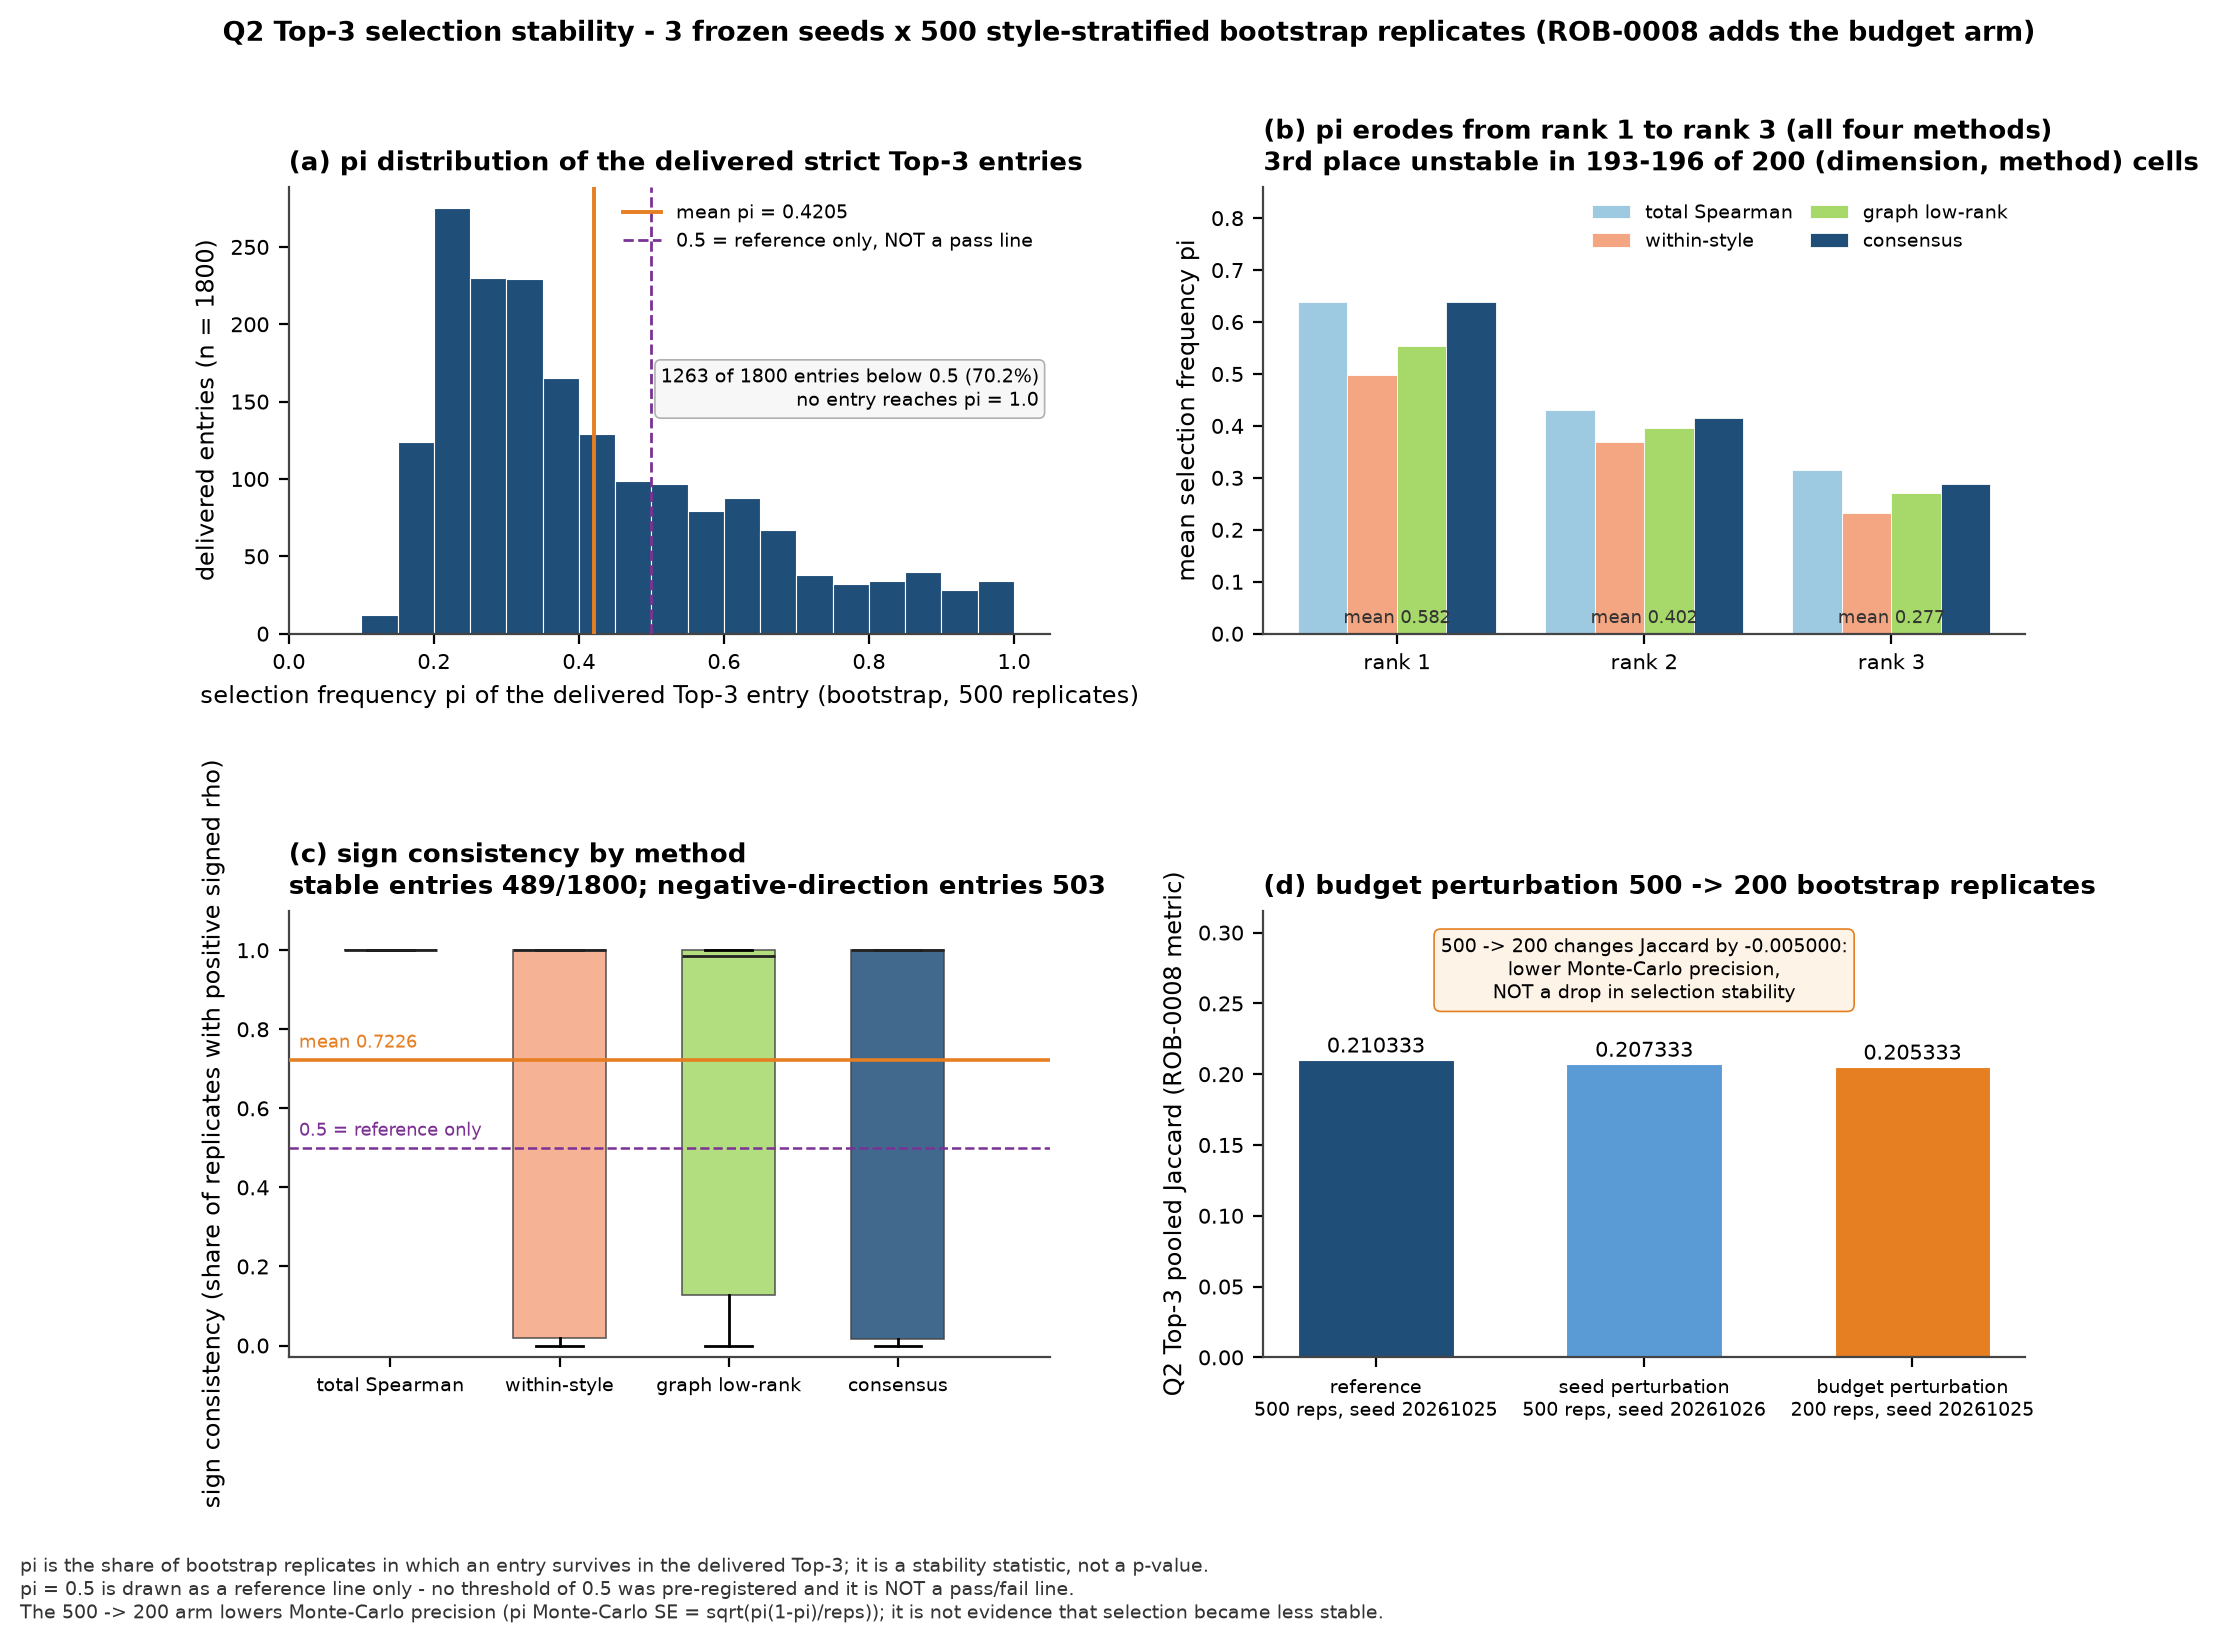
\includegraphics[width=0.92\linewidth,height=0.42\textheight,keepaspectratio]{../figures/confirmatory/Q2-stability.png}
\captionof{figure}{问题二：Top-3 入选频率 π 与符号一致性（500 次风格内 bootstrap、3 重复）；0.5 仅参考非判定，500→200 为蒙特卡洛精度变化。（\texttt{FIG-0036}）}
\end{bpfigure}

方向一致性方面，符号一致性均值为
0.7225544444444444：约四分之一的（候选，维度）组合在重抽样中改变了关联符号方向。这些组合的方向标签应视为不稳定，不应据此作机制解释。

附件 \texttt{6.csv} 提供 44 行化学---感官交叉相关，可匹配 44
行。按名称对齐后的平均秩相关为 0.9210176180408739（严格表
0.9080152788388083）。这一对照有两个限制：其一，该表与本研究使用同一批附件，属\textbf{同源对照}，不是外部验证集；其二，比较使用绝对关联排序，只能说明排序强度一致，不能说明方向正确。按位置对齐得到的旧值曾明显偏低，那正是列错位三列造成的度量结果，已作为历史记录保留，不再作为证据。

\subsection{化学合理性：机理支持与关联标志分层}\label{ux5316ux5b66ux5408ux7406ux6027ux673aux7406ux652fux6301ux4e0eux5173ux8054ux6807ux5fd7ux5206ux5c42}

\textbf{酯类与果香。}
乙酸异戊酯、乙酸乙酯等是酵母发酵相关的酯类，支持``酯香候选以酯类为主''的类别解释。已有啤酒化学---感官研究也显示酯类与醇类共同变化，单一变量的重要性可能替代与其共相关的其他化合物
{[}2{]}。因此若某维 Top-3
出现非酯类条目（例如醛类），应解释为代谢或工艺关联标志，而不是由排序直接推导添加效果。\textbf{该解释在本数据上属待证}：本文没有做加标或酿造干预实验。

\textbf{萜烯类与酒花柑橘、花香。}
香茅醇与香叶醇具有明确的描述词一致性，萜烯可随酒花或香料原料引入，风格差异也可能改变其出现方式
{[}2{]}。表 q2-core-top3
中凡被标为``混''的候选，说明其排序不能脱离配方与风格解释；本文不对其作用强弱排序。

\textbf{高级醇、有机酸与醇厚、酸感。}
甘油等成分可与口感联系，有机酸与酸感具有类别上的一致性 {[}2{]}。但未进入
Top-3
的已知风味物质不能据此排除，共线候选之间的名次差也不等于物质作用强弱。

\textbf{硫化物、双乙酰与缺陷。} 双乙酰可由发酵产生的前体
\(\alpha\)-乙酰乳酸转化，酵母也参与其还原去除 {[}3{]}；DMS
既有热过程前体途径，也可由发酵中 DMSO 还原产生
{[}4{]}。这些独立机理支持把双乙酰与 DMS
作为缺陷监测对象，但本问的统计排序与已知直接致味物并非一一对应；因此问题三直接约束已测得的
DMS、双乙酰与 4VG，而不以 Top-3 替代缺陷化学检测。

\subsection{问题二的作用边界}\label{ux95eeux9898ux4e8cux7684ux4f5cux7528ux8fb9ux754c}

第一，同期关联不等于因果。全部结果都是同一批样本上的同期关系，任何``某化合物决定某风味''的表述都不成立；Top-3
是排序假设，需独立干预实验检验。

第二，集合一致性不等于识别准确率。方法间 Jaccard 与跨重复 Jaccard
描述的是不同方法、不同重抽样下的排序分歧度，没有真值可以对照。

第三，同源对照不是外部验证。\texttt{6.csv}
与主数据来自同一批附件，其一致性只说明处理流程没有把排序弄乱，不能作为独立验证。

第四，预算扰动会同时影响 \(\pi\) 与 Jaccard。稳健性检验把 bootstrap
次数由 500 降到 200，Monte-Carlo
精度随之下降；该项检验的极差因此混入抽样精度变化，不能与``候选选择是否稳定''混为一谈。固定种子的复跑与外层结果逐位一致，只证明确定性重现。

\section{问题三：风格条件生成与声明模型下的迁移}\label{ux95eeux9898ux4e09ux98ceux683cux6761ux4ef6ux751fux6210ux4e0eux58f0ux660eux6a21ux578bux4e0bux7684ux8fc1ux79fb}

问题三包含两个不同对象：其一是按风格生成化学谱的条件生成器，其二是把
Pils/Lager 谱在声明约束下迁移到 Tripel
的优化算子。两者的指标、失败模式与边界都不同，本文分开评价，不合并为单一的``问题三成功率''。

\subsection{生成目标与评价对象}\label{ux751fux6210ux76eeux6807ux4e0eux8bc4ux4ef7ux5bf9ux8c61}

主任务学习已出现风格的条件分布 \(p(X\mid s)\)。采用固定 3
折风格内留出：每次重复的 22 个风格各自 3 折，共 198
个设计格；三次重复共生成 750
份谱。分布质量的能量距离只在\textbf{可估格}上计算：21 个可估风格共 177
个可估格、729 份可估生成样本（三次重复合计），另有 21 个格及其 21
份生成样本因对照侧样本不足被排除在能量距离之外并单列报告。设计格总数为
198、生成样本总数为 750；729 与 750
的差额即被排除部分，两者不可互换。标签不进入化学边际或 Copula
的似然拟合，只用于独立的感官代理与评价。

\subsection{原始抽样与约束设计谱的分离}\label{ux539fux59cbux62bdux6837ux4e0eux7ea6ux675fux8bbeux8ba1ux8c31ux7684ux5206ux79bb}

本轮同时保存两份谱：\texttt{raw} 为条件生成的原始抽样，\texttt{design}
为约束投影后的设计谱。分离二者的直接目的是让投影代价可测量，而不是只报告投影后的结果。33
个已校准线性列在抽样层就施加物理非负下界，因此原始抽样与设计谱的负浓度格数均为零；这一点是构造保证，不是``生成质量好''的证据。

\begin{bptable}
\setcounter{table}{8}
%% table-id: q3-raw-design sha256:b8e173bd751dd37412c631d52a05e58c592446805750db49ebfa18790a0b9bc1
\captionof{table}{原始抽样与约束设计谱的对照}\label{tab:q3-raw-design}
\par\smallskip
\small
\begin{tabular}{@{}>{\raggedright\arraybackslash}p{\dimexpr 0.2932\linewidth-6pt\relax}>{\raggedleft\arraybackslash}p{\dimexpr 0.1235\linewidth-6pt\relax}>{\raggedleft\arraybackslash}p{\dimexpr 0.1065\linewidth-6pt\relax}>{\raggedright\arraybackslash}p{\dimexpr 0.4448\linewidth-6pt\relax}@{}}
\toprule
指标 & 未约束原始生成 & 约束后设计谱 & 说明 \\
\midrule
归一化经验能量距离 V & 0.8843 & 0.8840 & 按 n\_\allowbreak{}gen 加权池化；越小表示生成谱越接近真实谱 \\
无符号能量 V & 16.1872 & 16.1828 & 非负的分布差异量 \\
带符号能量 U & 1.0881 & 1.1139 & 可负、不截零；负值表示生成谱在目标侧偏移 \\
约束满足率 & 0.1133 & 1.0000 & 同时满足全部声明约束的样本比例；设计侧由投影循环保证 \\
负浓度格数 & 0 & 0 & 线性非负约束被违反的格数 \\
约束投影轮数（均值） & — & 1.4798 & 逐格迭代直到最大残差 ≤ 1e-9，允许轮数上限 5 \\
约束投影轮数（最大） & — & 5 & 未超过允许轮数上限 \\
约束投影最大残差 & — & 0.0000 & 投影后从写出的样本文件复核 \\
全列平均绝对改动（标准化单位） & — & 0.0142 & 约束投影相对未约束原始抽样的逐列平均绝对改动 \\
改动最大的列：二甲基硫（DMS） & — & 0.5733 & 约束投影相对未约束原始抽样的逐列平均绝对改动 \\
改动最大的列：双乙酰（2,3-丁二酮） & — & 0.1920 & 约束投影相对未约束原始抽样的逐列平均绝对改动 \\
改动最大的列：反-2-壬烯醛 & — & 0.0571 & 约束投影相对未约束原始抽样的逐列平均绝对改动 \\
\bottomrule
\end{tabular}
\begin{tablenote}注：左侧为未施加约束的原始条件生成，右侧为约束投影后的设计谱。能量距离按可估格加权池化，V 与 U 是同一能量统计量的无符号与带符号读数；约束满足率在原始生成上几乎不成立，在设计谱上等于 1 是投影循环的构造性质，不能当作分布质量证据。改动量以标准化单位给出，只描述“投影改了多少”，不是约束残差。\end{tablenote}
\end{bptable}

两项必须分开读：归一化能量距离从原始抽样到设计谱的变化量测度的是``投影让分布偏离了多少''；而约束满足率从
0.11333333333333333 变为 1
是\textbf{构造性质}------设计谱由可行域投影产生，满足率必然为
1，它不提供任何关于真实酿造可行性的信息。未约束的原始抽样仅约一成满足全部声明约束，说明缺陷约束在实际生成中确实是有效约束，但这同样只是数学筛查。

\subsection{含编码质量点的层次收缩边际}\label{ux542bux7f16ux7801ux8d28ux91cfux70b9ux7684ux5c42ux6b21ux6536ux7f29ux8fb9ux9645}

对每个变量采用风格内经验边际与池化边际的层次收缩：

\[\bpMathFit{
\widehat F_{j,s}=\omega_s\widehat F^{\mathrm{emp}}_{j,s}+(1-\omega_s)\widehat F_j^{\mathrm{pool}},
\qquad \omega_s=\frac{n_s}{n_s+\kappa}.
}\]

有地板编码的变量另以混合分布保留编码质量点：

\[\bpMathFit{
F_{j,s}^{\mathrm{obs}}(v)=\pi_{j,s}^{\mathrm{floor}}\mathbf1\{v\ge v_j^{\mathrm{floor}}\}
+(1-\pi_{j,s}^{\mathrm{floor}})F_{j,s}^{\mathrm{nonfloor}}(v).
}\]

以相应概率抽取编码值，其余部分通过经验分位数插值采样。该结构避免把大量重复的地板值平滑成虚假的连续浓度：37
个对数列的 755 个校准零值与 142 列的 6807
个共享地板编码都作为质量点保留，而不是当作连续观测。

\subsection{收缩高斯 Copula}\label{ux6536ux7f29ux9ad8ux65af-copula}

将条件边际映射至高斯坐标，估计风格依赖结构：

\[\bpMathFit{
z_{ij}=\Phi^{-1}[\widehat F_{j,s_i}(x_{ij})],\quad
\widehat R_s=\eta_s\widehat R_s^{\mathrm{emp}}+(1-\eta_s)\widehat R_{\mathrm{shared}},
\quad \eta_s=\frac{n_s}{n_s+\kappa_R}.
}\]

相关矩阵特征值截断至至少 \(10^{-6}\)，归一化后再向单位阵收缩 5\%。采样
\(z^*\sim N(0,\widehat R_s)\)，经 \(u^*=\Phi(z^*)\) 与各条件逆边际得到
\(X^*\)。小样本风格更依赖池化信息，以减轻局部估计的不稳定。

参数选择在\textbf{每个外层折内部}用该折自己的 3
个内层折完成：\(\kappa\in\{0,5,15\}\)、\(\kappa_R\in\{20,50,100\}\) 的 9
个组合逐折选择，不跨折池化选择表，也不使用外层留出误差挑选参数。先导轮曾把逐折选择表平均后写回每一折，使该折的留出信息进入了自己的超参数；本轮已改为逐折独立选择。

\subsection{评价量：分布距离与结构统计}\label{ux8bc4ux4ef7ux91cfux5206ux5e03ux8dddux79bbux4e0eux7ed3ux6784ux7edfux8ba1}

归一化经验能量距离为

\[\bpMathFit{
\mathcal E^2_{\mathrm{norm}}=\frac{\max(\mathcal E^2,0)}{D_{\mathrm{ref}}},
\qquad
\mathcal E^2=2\mathbb E\|X-Y\|-\mathbb E\|X-X'\|-\mathbb E\|Y-Y'\|,
}\]

\(D_{\mathrm{ref}}\)
为同量真实训练样本的典型两两距离。同时报告两个能量统计量，二者语义不同：

\begin{itemize}
\tightlist
\item
  \(V=2\overline{d(G,R)}-\overline{d(G,G)}-\overline{d(R,R)}\)
  为经验能量距离，按构造非负，用于分布差异的强度；
\item
  \(U=2\overline{d(G,R)}-\overline{d(G,G)}-\overline{d(R,R)}\)
  为带符号诊断量，\textbf{可以为负}。\(U\)
  为负表示生成样本之间的离散程度低于参照，是``过度集中''的信号，本文不截零、不开方，也不把它当作距离使用。
\end{itemize}

此外分别报告边际误差、依赖谱
MAE、多样性（样本间平均距离）、最近邻距离、复制率与边饱和比例。它们各自回答一个问题，不能互相替代。

\subsection{生成质量与参照对照}\label{ux751fux6210ux8d28ux91cfux4e0eux53c2ux7167ux5bf9ux7167}

\begin{bptable}
\setcounter{table}{9}
%% table-id: q3-quality sha256:577eb42b7cbd5046d99de288c79061d5bcac7d7b53709e8d3387a1c29a1c4c1d
\captionof{table}{生成方案的分布质量与同协议参照对照}\label{tab:q3-quality}
\par\smallskip
\small
\begin{tabular}{@{}>{\raggedright\arraybackslash}p{\dimexpr 0.2132\linewidth-6pt\relax}>{\raggedleft\arraybackslash}p{\dimexpr 0.0918\linewidth-6pt\relax}>{\raggedleft\arraybackslash}p{\dimexpr 0.0855\linewidth-6pt\relax}>{\raggedleft\arraybackslash}p{\dimexpr 0.0966\linewidth-6pt\relax}>{\raggedleft\arraybackslash}p{\dimexpr 0.0966\linewidth-6pt\relax}>{\raggedleft\arraybackslash}p{\dimexpr 0.0855\linewidth-6pt\relax}>{\raggedleft\arraybackslash}p{\dimexpr 0.0855\linewidth-6pt\relax}>{\raggedright\arraybackslash}p{\dimexpr 0.2132\linewidth-6pt\relax}@{}}
\toprule
方案 & 归一化能量距离 V & 带符号 U & 多样性 & 最近邻距离 & 精确复制率 & 边饱和比例 & 范围说明 \\
\midrule
分层收缩混合 Copula 设计谱（主方案） & 0.8840 & 1.1139 & 19.7356 & 17.6323 & 0.0000 & 0.1199 & 能量/\allowbreak{}U/\allowbreak{}多样性/\allowbreak{}最近邻按 177 格 ·\allowbreak{} 729 份加权；复制率与边饱和按 231×750 格 \\
仅共享相关 Copula & 0.8870 & 1.1704 & 19.7374 & 17.7041 & 0.0000 & 0.1209 & 能量/\allowbreak{}U/\allowbreak{}多样性/\allowbreak{}最近邻按 177 格 ·\allowbreak{} 729 份加权；复制率与边饱和按 231×750 格 \\
风格内经验 Copula & 0.8711 & 1.0938 & 18.7862 & 15.6167 & 0.0000 & 0.1122 & 能量/\allowbreak{}U/\allowbreak{}多样性/\allowbreak{}最近邻按 177 格 ·\allowbreak{} 729 份加权；复制率与边饱和按 231×750 格 \\
独立边际 & 0.8853 & 1.0911 & 19.8522 & 18.6022 & 0.0000 & 0.1222 & 能量/\allowbreak{}U/\allowbreak{}多样性/\allowbreak{}最近邻按 177 格 ·\allowbreak{} 729 份加权；复制率与边饱和按 231×750 格 \\
源样本重采样参照 & 0.8137 & 0.1806 & 18.3913 & 16.0210 & 0.0000 & 0.1197 & 同风格训练行重采样参照，不是生成模型；能量/\allowbreak{}U/\allowbreak{}多样性/\allowbreak{}最近邻按 177 格 ·\allowbreak{} 729 份加权；复制率与边饱和按 231×750 格 \\
范围口径：21 个可估风格 ·\allowbreak{} 177 个可估格池化 & 0.8840 & — & — & — & — & — & n\_\allowbreak{}gen=729；与主方案同值，用于声明池化范围 \\
范围口径：Tripel/\allowbreak{}Kriek/\allowbreak{}Lambic 三风格 ·\allowbreak{} 27 个格单独池化 & 1.8306 & — & — & — & — & — & n\_\allowbreak{}gen=147；与上一行不是同一范围，不可互换 \\
\bottomrule
\end{tabular}
\begin{tablenote}注：前五行为同一评价协议下不同采样方案的设计谱比较，能量距离越小越好；U 可负、不截零。\textbf{分母不同，不可混读}：归一化能量距离、带符号 U、多样性与最近邻距离按 177 个可估格、729 份生成的 n\_gen 加权口径计算；精确复制率与边饱和比例的分母是 231×750 = 173250 个存储单元格（750 行），其中包含未进入能量距离的 21 个不可估格 / 21 份生成，因此两类指标的分母不是同一批格。四个分布侧指标各自回答不同问题，不可互相解释：多样性为生成样本在标准化空间中的两两欧氏距离均值（按固定抽样次数子采样）；最近邻距离为每个样本到最近样本距离的均值；精确复制率为与已有行完全重复的行占比；边饱和比例为落在声明边界上的单元格占比（地板编码、观测支撑上下界、线性列零值）。源样本重采样参照直接复用同风格的训练行，其能量距离低于各生成方案；该行的作用是给出“不生成”的参照，不能与生成模型等同比较。后两行只声明池化范围：21 个可估风格 177 个可估格的池化值与三风格单独池化值不可互换，引用时必须写明范围。\end{tablenote}
\end{bptable}

本表的读法是``与谁比''而不是``数值多大''。设计谱的归一化能量距离为
0.8840256215416039，无符号统计量 \(V=\) 16.182791432827685，带符号统计量
\(U=\) 1.1138668332620816（为正，表示生成样本比参照更分散）；多样性
19.735647194424246，最近邻距离 17.63230853329826，复制率 0，边饱和比例
0.11991341991341999。

关键对照是\textbf{源样本重采样}：同样本量、同风格、直接对训练行重采样得到的参照谱，其归一化能量距离低于生成设计谱（两者并列于表
q3-quality 的同协议对照行），而生成设计谱为
0.8840256215416039。也就是说，在本评价口径下，\textbf{生成器没有超过``直接重采样真实样本''这一最简参照}。这是本问最重要的负结果，本文据此明确不宣称生成模型优于基线。

\begin{bpfigure}
%% figure-id: FIG-0037 sha256:0e5d64be11e8a391a61de27e52838e8134661332d114d83cb314b2445a523349
%% figure-src: ../figures/confirmatory/Q3-energy-comparison.png
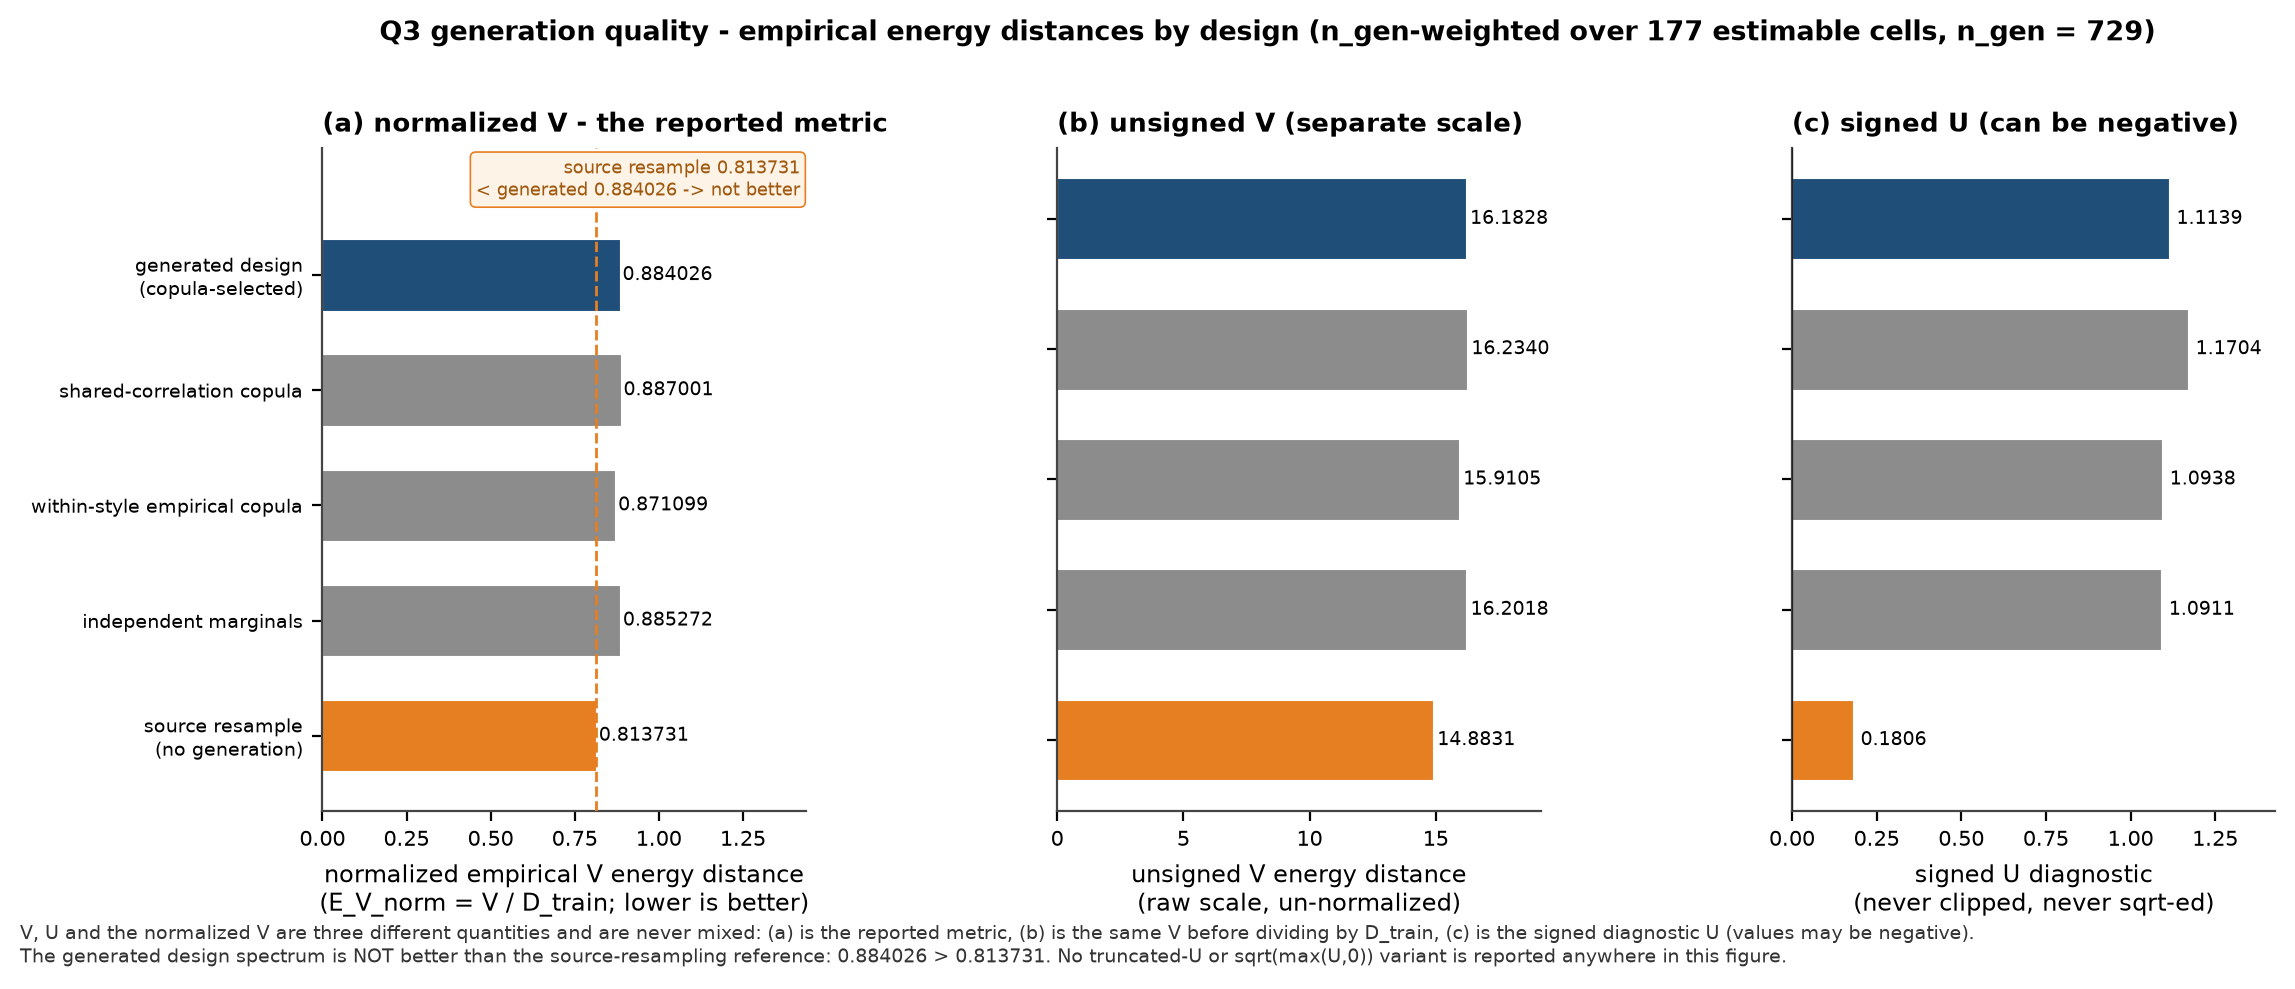
\includegraphics[width=0.92\linewidth,height=0.42\textheight,keepaspectratio]{../figures/confirmatory/Q3-energy-comparison.png}
\captionof{figure}{问题三：归一化经验 V 能量距离（V/D\_train）对照；生成设计谱 0.8840 未优于源样本重采样 0.8137，带符号 U 单列不截零。（\texttt{FIG-0037}）}
\end{bpfigure}

依赖结构方面，Copula 相对独立边际的收益体现在依赖谱
MAE（0.00699721596405482）与协方差迹比上；但三类 Copula
收缩方案之间的能量距离差异小于它们与源样本重采样参照的差异，因此``copula
结构选择''在本数据上不是主导因素。边际误差仍为
0.5097988519859696，说明单变量分布本身也未被完全复现。

\subsection{三种目标风格必须与池化结果分开}\label{ux4e09ux79cdux76eeux6807ux98ceux683cux5fc5ux987bux4e0eux6c60ux5316ux7ed3ux679cux5206ux5f00}

设计谱在 21 个可估风格的 177 个可估格上按生成样本数加权池化为
0.8840256215416039。但 Tripel、Kriek、Lambic 三种风格单独池化（27
个格、147
份生成样本）的值明显高于上述池化值------这是描述性差异，本文未对两个池化值作任何显著性检验，其数值见表
q3-quality 的三风格单独池化行。两者是不同
scope：前者是所有可估风格的平均表现，后者是三种小样本风格的表现。

因此本文\textbf{不得}用 21 风格池化值代替三风格画像的质量评价。Kriek
只有 10 行训练样本、Lambic 11 行、Tripel 28
行（另加留出槽位），收缩强度大，池化后的小风格差异被平均掉，单独计算时会暴露。

\begin{bpfigure}
%% figure-id: FIG-0038 sha256:6ef2bac1b7b9b8867864f3fc8df85a3f24fdfc9f066e0488c4e2b57678959a6b
%% figure-src: ../figures/confirmatory/Q3-per-style-energy.png
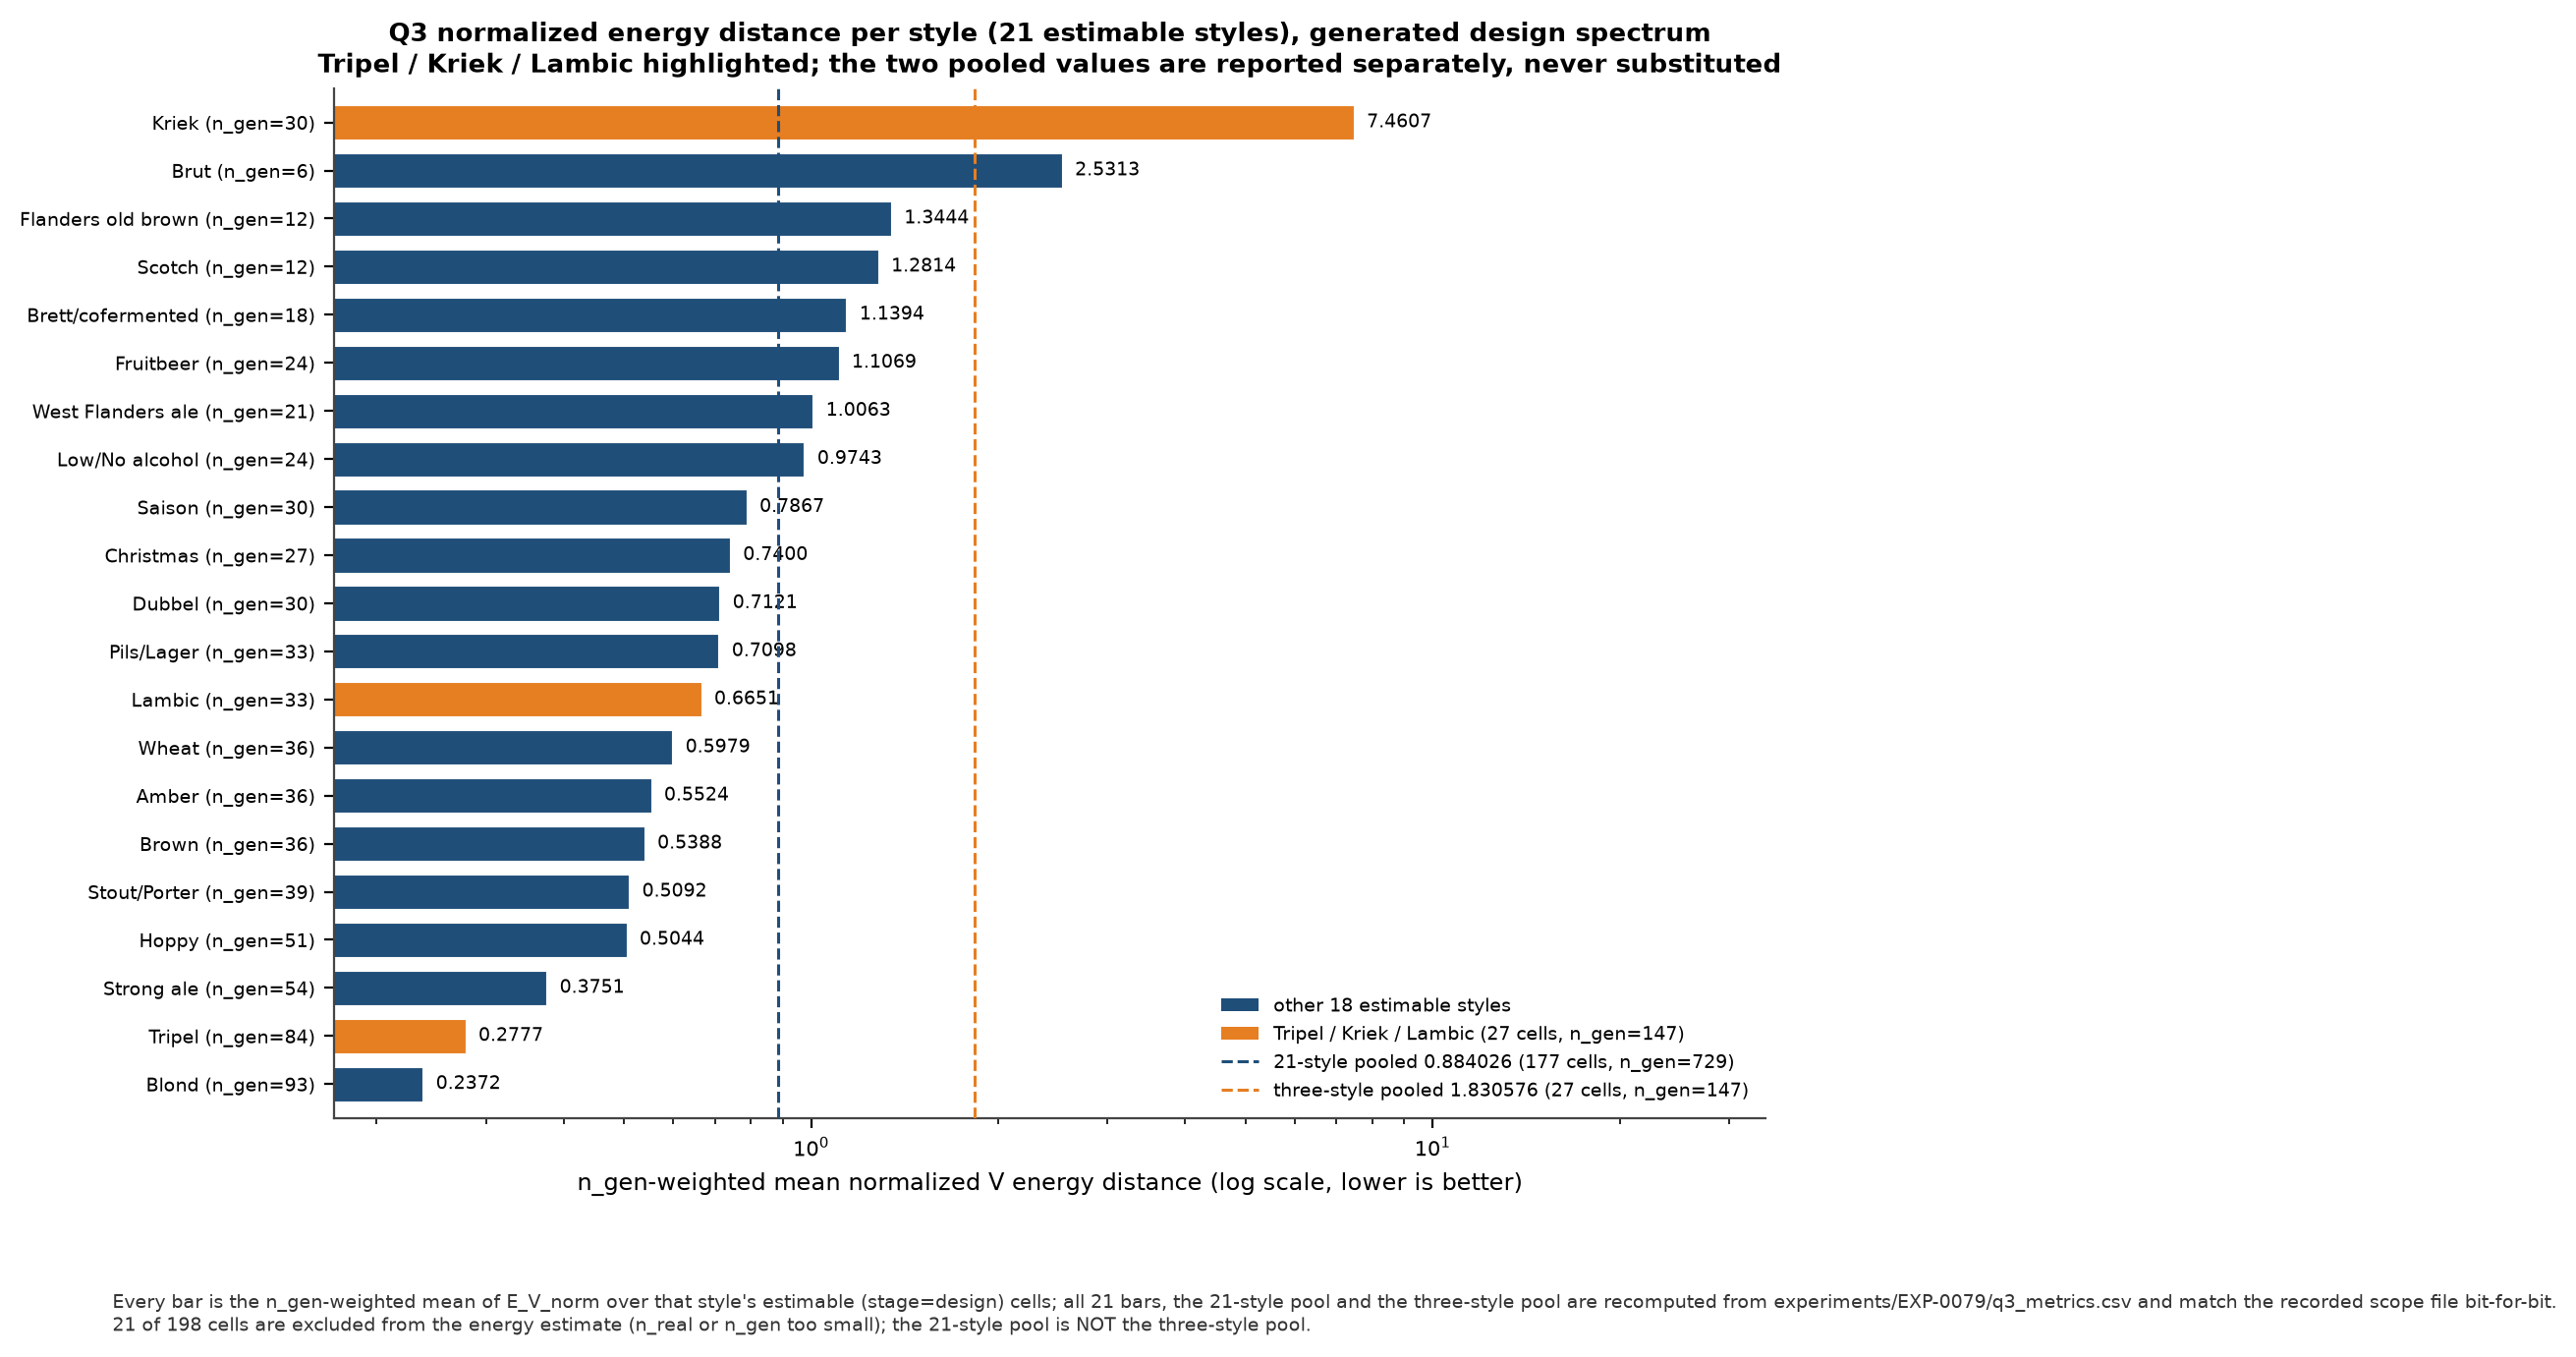
\includegraphics[width=0.92\linewidth,height=0.42\textheight,keepaspectratio]{../figures/confirmatory/Q3-per-style-energy.png}
\captionof{figure}{问题三：逐风格 n\_gen 加权能量距离（21 可估风格）；三风格池化 1.8306 与 21 风格池化 0.8840 分列标注、不得互替。（\texttt{FIG-0038}）}
\end{bpfigure}

\begin{bptable}
\setcounter{table}{10}
%% table-id: q3-constraints sha256:69b722d61b523aa767a6d1f81499afca2129210a7e2b41fd2c2a9291f9826a8d
\captionof{table}{声明约束的核验构成}\label{tab:q3-constraints}
\par\smallskip
\small
\begin{tabular}{@{}>{\raggedright\arraybackslash}p{\dimexpr 0.6751\linewidth-6pt\relax}>{\raggedleft\arraybackslash}p{\dimexpr 0.1434\linewidth-6pt\relax}>{\raggedleft\arraybackslash}p{\dimexpr 0.1495\linewidth-6pt\relax}@{}}
\toprule
核验状态 & 记录数 & 占比 \\
\midrule
已验证（verified） & 19619 & 0.6884 \\
条件成立（conditional） & 8201 & 0.2878 \\
不可识别（not identifiable） & 680 & 0.0239 \\
不可行（infeasible） & 0 & 0.0000 \\
合计 & 28500 & 1.0000 \\
\bottomrule
\end{tabular}
\par\smallskip
\begin{tabular}{@{}>{\raggedright\arraybackslash}p{\dimexpr 0.4934\linewidth-6pt\relax}>{\raggedleft\arraybackslash}p{\dimexpr 0.0848\linewidth-6pt\relax}>{\raggedleft\arraybackslash}p{\dimexpr 0.0848\linewidth-6pt\relax}>{\raggedleft\arraybackslash}p{\dimexpr 0.1113\linewidth-6pt\relax}>{\raggedleft\arraybackslash}p{\dimexpr 0.1107\linewidth-6pt\relax}>{\raggedleft\arraybackslash}p{\dimexpr 0.0831\linewidth-6pt\relax}@{}}
\toprule
约束类 & 记录数 & 已验证 & 条件成立 & 不可识别 & 不可行 \\
\midrule
缺陷硬阈值·\allowbreak{}二甲基硫上界 & 750 & 750 & 0 & 0 & 0 \\
缺陷硬阈值·\allowbreak{}4-乙烯基愈创木酚上界 & 750 & 256 & 0 & 494 & 0 \\
缺陷硬阈值·\allowbreak{}双乙酰上界 & 750 & 0 & 750 & 0 & 0 \\
反-2-壬烯醛化学不增（训练 q90 上界） & 750 & 0 & 750 & 0 & 0 \\
老化酒花代理上界（岭回归代理） & 750 & 0 & 750 & 0 & 0 \\
线性非负（33 列） & 24750 & 18613 & 5951 & 186 & 0 \\
合计 & 28500 & 19619 & 8201 & 680 & 0 \\
\bottomrule
\end{tabular}
\begin{tablenote}注：上表为逐条约束记录的四类核验状态，下表按约束类拆分。“已验证”指约束在写出的样本文件中被直接复核；“条件成立”指约束依赖训练折内的数据派生界或代理变量；“不可识别”指该格的上界无法从数据确定（如缺陷列缺测）；不可行记录为零。设计谱的约束满足率为 1.0000（由约束投影保证），未约束原始生成仅 0.1133；核验记录合计 28500 条，其中已验证占比 0.6884。线性非负类覆盖 33 个化学列；老化酒花只有训练折内的代理约束，不能读作实测老化指标。\end{tablenote}
\end{bptable}

约束核验共 19619 项通过、8201 项条件成立、680 项不可辨识、0
项不可行。不可辨识项主要来自未校准变量：其观测支撑不足以判定物理阈值是否满足，本文把它们计为不可辨识而不是计为通过。``条件成立''指满足程度依赖于已声明的编码约定（例如地板编码计作零浓度），该约定在附录说明。

\subsection{迁移：变量空间、目标与约束}\label{ux8fc1ux79fbux53d8ux91cfux7a7aux95f4ux76eeux6807ux4e0eux7ea6ux675f}

迁移只在声明的凸二次规划下成立，因此必须把``模型''写全。对每个外层折，目标风格的参照只由该折\textbf{目标风格的训练行}定义：目标均值、目标主成分与目标相关矩阵、以及感官代理，全部只用训练行估计。源风格样本是\textbf{查询输入}，源风格从所有拟合中排除。

变量取折叠标准化的存储空间 \(z\in\mathbb R^{231}\)。声明的二次规划为

\[\bpMathFit{
\min_{z,t}\ (z-z_{\mathrm{ref}})^\top Q_t(z-z_{\mathrm{ref}})
+\lambda\|z-z_{\mathrm{anchor}}\|_2^2+\eta\sum_k t_k
\quad\text{s.t.}\quad
-t\le z-z_{\mathrm{source}}\le t,\ \ t\ge0,\ \ l\le z\le u,\ \ Az\le b,
}\]

其中
\(Q_t=P^\top\operatorname{diag}(1/s_d)^2\Sigma_{\mathrm{corr}}^{-1}\operatorname{diag}(1/s_d)^2P\)
为秩 10 的目标主成分二次型（\(P\)
为目标风格主成分载荷，\(\Sigma_{\mathrm{corr}}\) 取
\(0.9\widehat R_T+0.1I\) 的收缩形式），\(z_{\mathrm{anchor}}\)
为分位数保序锚点；\(\eta>0\) 时最优解满足
\(t=|z-z_{\mathrm{source}}|\)，故 \(t\) 在最优处消去。盒约束 \(l,u\)
承载声明支撑与四条逐坐标化学上限（DMS、双乙酰、4VG、反式-2-壬烯醛均不得高于源样本），\(Az\le b\)
是唯一一条 \texttt{stale\_hops}
线性代理行------它是\textbf{代理}，不是实测化学约束。

求解采用精确的 ADMM
原-对偶方法：盒约束与单条半空间约束的投影用二分法，秩 10 二次型用
Woodbury
恒等式求逆。较通用的序列二次规划解法在本问题上被基准比较后弃用（单次求解约
27 秒、状态码 8、残差约 \(10^{-4}\)，变量 462
个）。每个求解写入证书：问题哈希、状态、目标值、原残差、对偶残差、迭代数、可行性核验与
KKT 平稳性核验。目标梯度另与中心差分交叉核对，唯一允许的偏差是
\(|z-z_{\mathrm{source}}|=0\) 处的 \(L_1\) 折点，该处已单独报告与解释。

若某次求解未达到容差，交付点回退到源样本点，并记为``迁移未完成''，\textbf{不计入成功}。本轮所有
198 次求解均报告最优，没有发生回退。

\subsection{求解证书与独立复算}\label{ux6c42ux89e3ux8bc1ux4e66ux4e0eux72ecux7acbux590dux7b97}

\begin{bpLTsmall}
\setcounter{table}{11}
\begin{longtable}{@{}>{\raggedright\arraybackslash}p{\dimexpr 0.3210\linewidth-6pt\relax}>{\raggedleft\arraybackslash}p{\dimexpr 0.1191\linewidth-6pt\relax}>{\raggedright\arraybackslash}p{\dimexpr 0.5279\linewidth-6pt\relax}@{}}
%% table-id: q3-qp-certs sha256:457b2cda6ae36354c3f99974b9a8a900a33a648fc2d337134551e6096671b451
\caption{二次规划求解证书摘要}\label{tab:q3-qp-certs}\\
\toprule
指标 & 数值 & 口径与说明 \\
\midrule
\endfirsthead
\toprule
指标 & 数值 & 口径与说明 \\
\midrule
\endhead
\bottomrule
\endfoot
QP 求解次数 & 198 & 两种锚定策略分别 99 /\allowbreak{} 99 次 \\
状态 optimal & 198 & solver 返回最优 \\
状态 infeasible & 0 & 声明可行域内未出现不可行问题 \\
状态 未收敛 & 0 & 未出现未收敛 \\
唯一问题哈希数 & 198 & 逐问题哈希互不相同，说明 198 个问题各自独立 \\
最大原始残差 & 9.99e-09 & ADMM 一致性分裂的 max |z − w| \\
最大对偶残差 & 3.394e-10 & 缩放对偶残差 rho·\allowbreak{}max|w\_\allowbreak{}k − w\_\{k−1\}| \\
最大约束违反 & 0.0000 & box 界与半空间约束的违反量 \\
最大 KKT 平稳性残差 & 5.617e-09 & 平滑梯度 + L1 次梯度 + 紧约束乘子的平稳性 \\
目标梯度有限差分最大绝对差 & 4.493e-09 & 198 个检查点的最大值 \\
目标梯度有限差分最大相对差 & 8.357e-06 & 同一批检查点 \\
策略分布 & 99 /\allowbreak{} 99 & QP·\allowbreak{}源锚定 /\allowbreak{} QP·\allowbreak{}分位数锚定 \\
最大迭代次数 & 49 & ADMM 迭代上限内收敛 \\
内部不一致记录 & 0 & 证书字段之间的自洽检查 \\
\end{longtable}
\begin{tablenote}注：本表是 198 个逐问题凸二次规划证书的汇总，不是原生优化验证，也不保证全局最优之外的任何性质。残差是求解器收敛读数，不是迁移准确率；约束违反为 0 说明解在声明的可行域内，可行域本身（box 界、一条半分空间、秩 10 二次目标与两处正则项）由模型声明固定。目标梯度有限差分只核对实现中的梯度与目标函数一致。\end{tablenote}
\end{bpLTsmall}

198 次求解全部状态为最优（198），最大原残差
9.989717497660422e-9、最大对偶残差 3.393784142602385e-10、最大约束违反
0，均远低于声明可行性容差
\(10^{-8}\)。目标梯度与中心差分的最大绝对偏差为 4.493432292917987e-9。

这些证书另经独立复算脚本从头重算：198 个证书状态均为最优、198
个问题哈希互不相同、约束违反为零、原残差与对偶残差复算一致；代理行有
4/396 行出现 \(10^{-9}\) 量级差异，原因是记录端使用
\(\max(0,\Delta-10^{-9})\) 而审计端使用
\(\max(0,\Delta)\)，该差异已披露而非掩盖。需要强调：\textbf{证书只证明``求解器在声明模型下找到了满足
KKT
的点''，不证明该模型是真实迁移过程，也不构成原生的优化验证项}。本实验未声明优化参数，工具据此对优化可行性检查与优化目标检查给出具名拒绝，本文不声称通过。

\subsection{不增率的饱和性与 58
条代理越界}\label{ux4e0dux589eux7387ux7684ux9971ux548cux6027ux4e0e-58-ux6761ux4ee3ux7406ux8d8aux754c}

\begin{bptable}
\setcounter{table}{12}
%% table-id: q3-transfer-stages sha256:361b6f06bf5e18b3e97516b09cdba08fd74fcaf1955fdbab9a6e269c817fa369
\captionof{table}{四种迁移策略的阶段指标}\label{tab:q3-transfer-stages}
\par\smallskip
\small
\begin{tabular}{@{}>{\raggedright\arraybackslash}p{\dimexpr 0.1705\linewidth-6pt\relax}>{\raggedleft\arraybackslash}p{\dimexpr 0.0855\linewidth-6pt\relax}>{\raggedleft\arraybackslash}p{\dimexpr 0.0855\linewidth-6pt\relax}>{\raggedleft\arraybackslash}p{\dimexpr 0.1204\linewidth-6pt\relax}>{\raggedleft\arraybackslash}p{\dimexpr 0.1330\linewidth-6pt\relax}>{\raggedleft\arraybackslash}p{\dimexpr 0.1456\linewidth-6pt\relax}>{\raggedleft\arraybackslash}p{\dimexpr 0.1086\linewidth-6pt\relax}>{\raggedleft\arraybackslash}p{\dimexpr 0.1187\linewidth-6pt\relax}@{}}
\toprule
策略 & 转移能量 V & 归一化 V & 四条化学列不增率 & 老化酒花代理不增率 & 综合不增率（含代理） & fallback 份额 & 目标均值自距 \\
\midrule
QP·\allowbreak{}分位数锚定（交付策略） & 2.2611 & 0.1236 & 1.0000 & 1.0000 & 1.0000 & 0.0000 & — \\
QP·\allowbreak{}源锚定 & 7.2406 & 0.3984 & 1.0000 & 1.0000 & 1.0000 & 0.0000 & — \\
源固定（平凡对照） & 7.1963 & 0.3958 & 1.0000 & 1.0000 & 1.0000 & 0.0000 & — \\
目标均值投影（参照控制） & 6.9415 & 0.3794 & 1.0000 & 0.4141 & 0.4141 & 0.0000 & 4.749e-16 \\
\bottomrule
\end{tabular}
\begin{tablenote}注：转移能量按同一批目标参考行计算，越小表示迁移后的谱越接近目标风格。四条化学列不增率只统计二甲基硫、双乙酰、4-乙烯基愈创木酚、反-2-壬烯醛四条 cap；综合不增率另要求老化酒花代理不增。目标均值投影的综合值偏低完全由代理越界驱动，其四条化学 cap 仍全部满足，因此“综合不增率 0.4141”不等于“四条 cap 有 58\% 不满足”。源固定策略是不做任何迁移的平凡对照，其四条化学列与综合不增率同样为 1，因此不能把 1.000 读成迁移效果；老化酒花代理是训练折内的岭回归代理，不是实测老化指标。该复合指标在稳健性检验的三次运行中均为 1.000（有界饱和），min-value 规则下“min 1 ≥ 1”不构成改善或强稳健证据。目标均值投影是参照控制，其代理越界记录只属该参照控制，不参与交付判定。fallback 份额为 0 表示没有迁移结果被退回源谱。目标均值自距是“目标均值到自身”的距离，只对目标均值投影策略有意义；早期中心化口径下的同名值偏大，已被修复，不再引用。\end{tablenote}
\end{bptable}

先分清两个量（该复合指标在台账中旧称``逐列不增率''，本文统一称``综合不增率''）。\textbf{四条化学列（DMS、双乙酰、4VG、反-2-壬烯醛）的不增率}在四种策略下\textbf{都是}
1（表 q3-transfer-stages 的``四条化学列不增率''列）：无论 QP
策略、平凡对照还是参照控制，四条 cap
都没有被违反。\textbf{综合不增率}另要求 \texttt{stale\_hops}
代理不增，\texttt{qp-\allowbreak{}quantile-\allowbreak{}anchor}、\texttt{qp-\allowbreak{}source-\allowbreak{}anchor} 与
\texttt{source-fixed} 的综合值均为 1，而 \texttt{target-\allowbreak{}mean-\allowbreak{}projection}
参照控制的综合值为
0.41414141414141414------这一低值\textbf{完全由代理上限的越界驱动}，不是化学
cap 失败。

三个策略的综合 1.000
也必须一起读，因为其中一个是\textbf{平凡对照}：\texttt{source-fixed}
不改变任何化学值，其不增率必然为
1。因此``1.000''不能区分``优化真的找到更好的可行点''与``根本没有移动''。

更根本的问题是\textbf{指标饱和}：不增率是硬上界约束的直接结果，\(c^{\mathrm{new}}\le c^{\mathrm{source}}\)
逐列成立时该比值恒为 1，其取值上界就是
1，没有改善空间。稳健性检验中三次运行的不增率都是 1.000、极差为
0，这同样不提供信息------它只是再次确认约束被构造性满足，不能读成``强稳健性''或``改善量''。

关于 58 条越界：全部越界项都来自 \texttt{stale\_hops}
的岭代理、界限类型为源值上限代理，且\textbf{只出现在
\texttt{target-\allowbreak{}mean-\allowbreak{}projection} 这一参照控制中}；两个 QP
策略下越界数为零。残差和完全由这 58 条构成，与 198 个 QP
的盒约束加半空间约束的 \texttt{max\_constraint\_violation=0}
不是同一对象。把二者混写会把``参照控制的代理越界''误报成``QP
硬约束失败''。

\subsection{位移、约束残差与 z
空间位移是三组不同的量}\label{ux4f4dux79fbux7ea6ux675fux6b8bux5deeux4e0e-z-ux7a7aux95f4ux4f4dux79fbux662fux4e09ux7ec4ux4e0dux540cux7684ux91cf}

\begin{bptable}
\setcounter{table}{13}
%% table-id: q3-transfer-columns sha256:97874c0dfba5c3aa03f638aa78c6082f87f9dafaa40773e13fe4f50b783f77c1
\captionof{table}{关键列的三组量：约束残差、存储空间位移与 z 空间位移}\label{tab:q3-transfer-columns}
\par\smallskip
\small
\begin{tabular}{@{}>{\raggedright\arraybackslash}p{\dimexpr 0.2569\linewidth-6pt\relax}>{\raggedleft\arraybackslash}p{\dimexpr 0.1193\linewidth-6pt\relax}>{\raggedleft\arraybackslash}p{\dimexpr 0.1501\linewidth-6pt\relax}>{\raggedleft\arraybackslash}p{\dimexpr 0.1614\linewidth-6pt\relax}>{\raggedleft\arraybackslash}p{\dimexpr 0.1358\linewidth-6pt\relax}>{\raggedleft\arraybackslash}p{\dimexpr 0.1445\linewidth-6pt\relax}@{}}
\toprule
对象 & ①约束残差 max & ②存储空间位移 max & ②存储空间位移 mean & ③z 空间位移 max & ③z 空间位移 mean \\
\midrule
反-2-壬烯醛 & 3.556e-17 & 0.0010 & 1.019e-05 & — & — \\
双乙酰 & 1.804e-16 & 0.5239 & 0.0939 & — & — \\
4-乙烯基愈创木酚 & 0.0000 & 0.3233 & 0.0127 & — & — \\
z 空间·\allowbreak{}逐行 231 维绝对位移均值 & — & — & — & 0.6429 & 0.4994 \\
z 空间·\allowbreak{}逐行 231 维 L1 位移 & — & — & — & 148.5148 & 115.3690 \\
\bottomrule
\end{tabular}
\begin{tablenote}注：三组量不是同一对象，不能相互替代或相减。①约束残差是上限约束下 clamp(新值 − 源值, 0) 的逐行最大值，量级在浮点误差附近，只说明约束未被违反；②存储空间位移是 |新值 − 源值| 的逐列最大/均值，描述配方改动了多少；③z 空间位移是 231 维中心化标准化后的逐行位移，逐列分解未随产物保存，故只给出行级读数。z 空间读数已由独立重算复核，逐行一致。三组都只针对交付的 QP 分位数锚定策略。\end{tablenote}
\end{bptable}

第一组是\textbf{约束残差}：\(\operatorname{clamp}(x^{\mathrm{new}}-x^{\mathrm{source}},0)\)
的最值（表 q3-transfer-columns
第一组）。该组量的量级就是数值零，它回答``约束是否被违反''，不回答``改动了多少''。

第二组是\textbf{存储空间位移}：\texttt{qp-\allowbreak{}quantile-\allowbreak{}anchor}
策略的逐列位移最值与均值（表 q3-transfer-columns
第二组）。反式-2-壬烯醛的位移极小却仍报出非零残差，正是因为该列位移本身接近数值噪声；三个关键列的位移量级差异很大，不能用单一``平均改动''概括。

这里必须补一个范围说明：表 q3-transfer-columns
只发布与缺陷约束直接相关的三列，而 231
列的整体位移由痕量化合物主导，其存储尺度最大位移远大于这三列（逐列分布见图
Q3-transfer-shift 的第 (1)
组）。因此这三列的位移\textbf{不代表}整体设计位移，也不能反过来用整体位移的尺度去判断缺陷约束是否被满足------后者只看约束残差。

第三组是 \textbf{z 空间位移}：用冻结快照与确定性代码重建 9
组中心与尺度后，396 行 \(L_1\) 改动与平均绝对改动全部复算一致（逐行差为
0）。这证明该位移可复现，\textbf{不}证明目标函数或最优性正确。三组量分别回答``是否越界''\,``改了多少（存储尺度）''\,``改了多少（标准化尺度）''，混写会同时高估约束违反与低估改动。

\begin{bpfigure}
%% figure-id: FIG-0039 sha256:3c982d2394e3900ef7c91fd4f051d75ba8fd4e48123f9f548ae16efef9ba1e52
%% figure-src: ../figures/confirmatory/Q3-transfer-shift.png
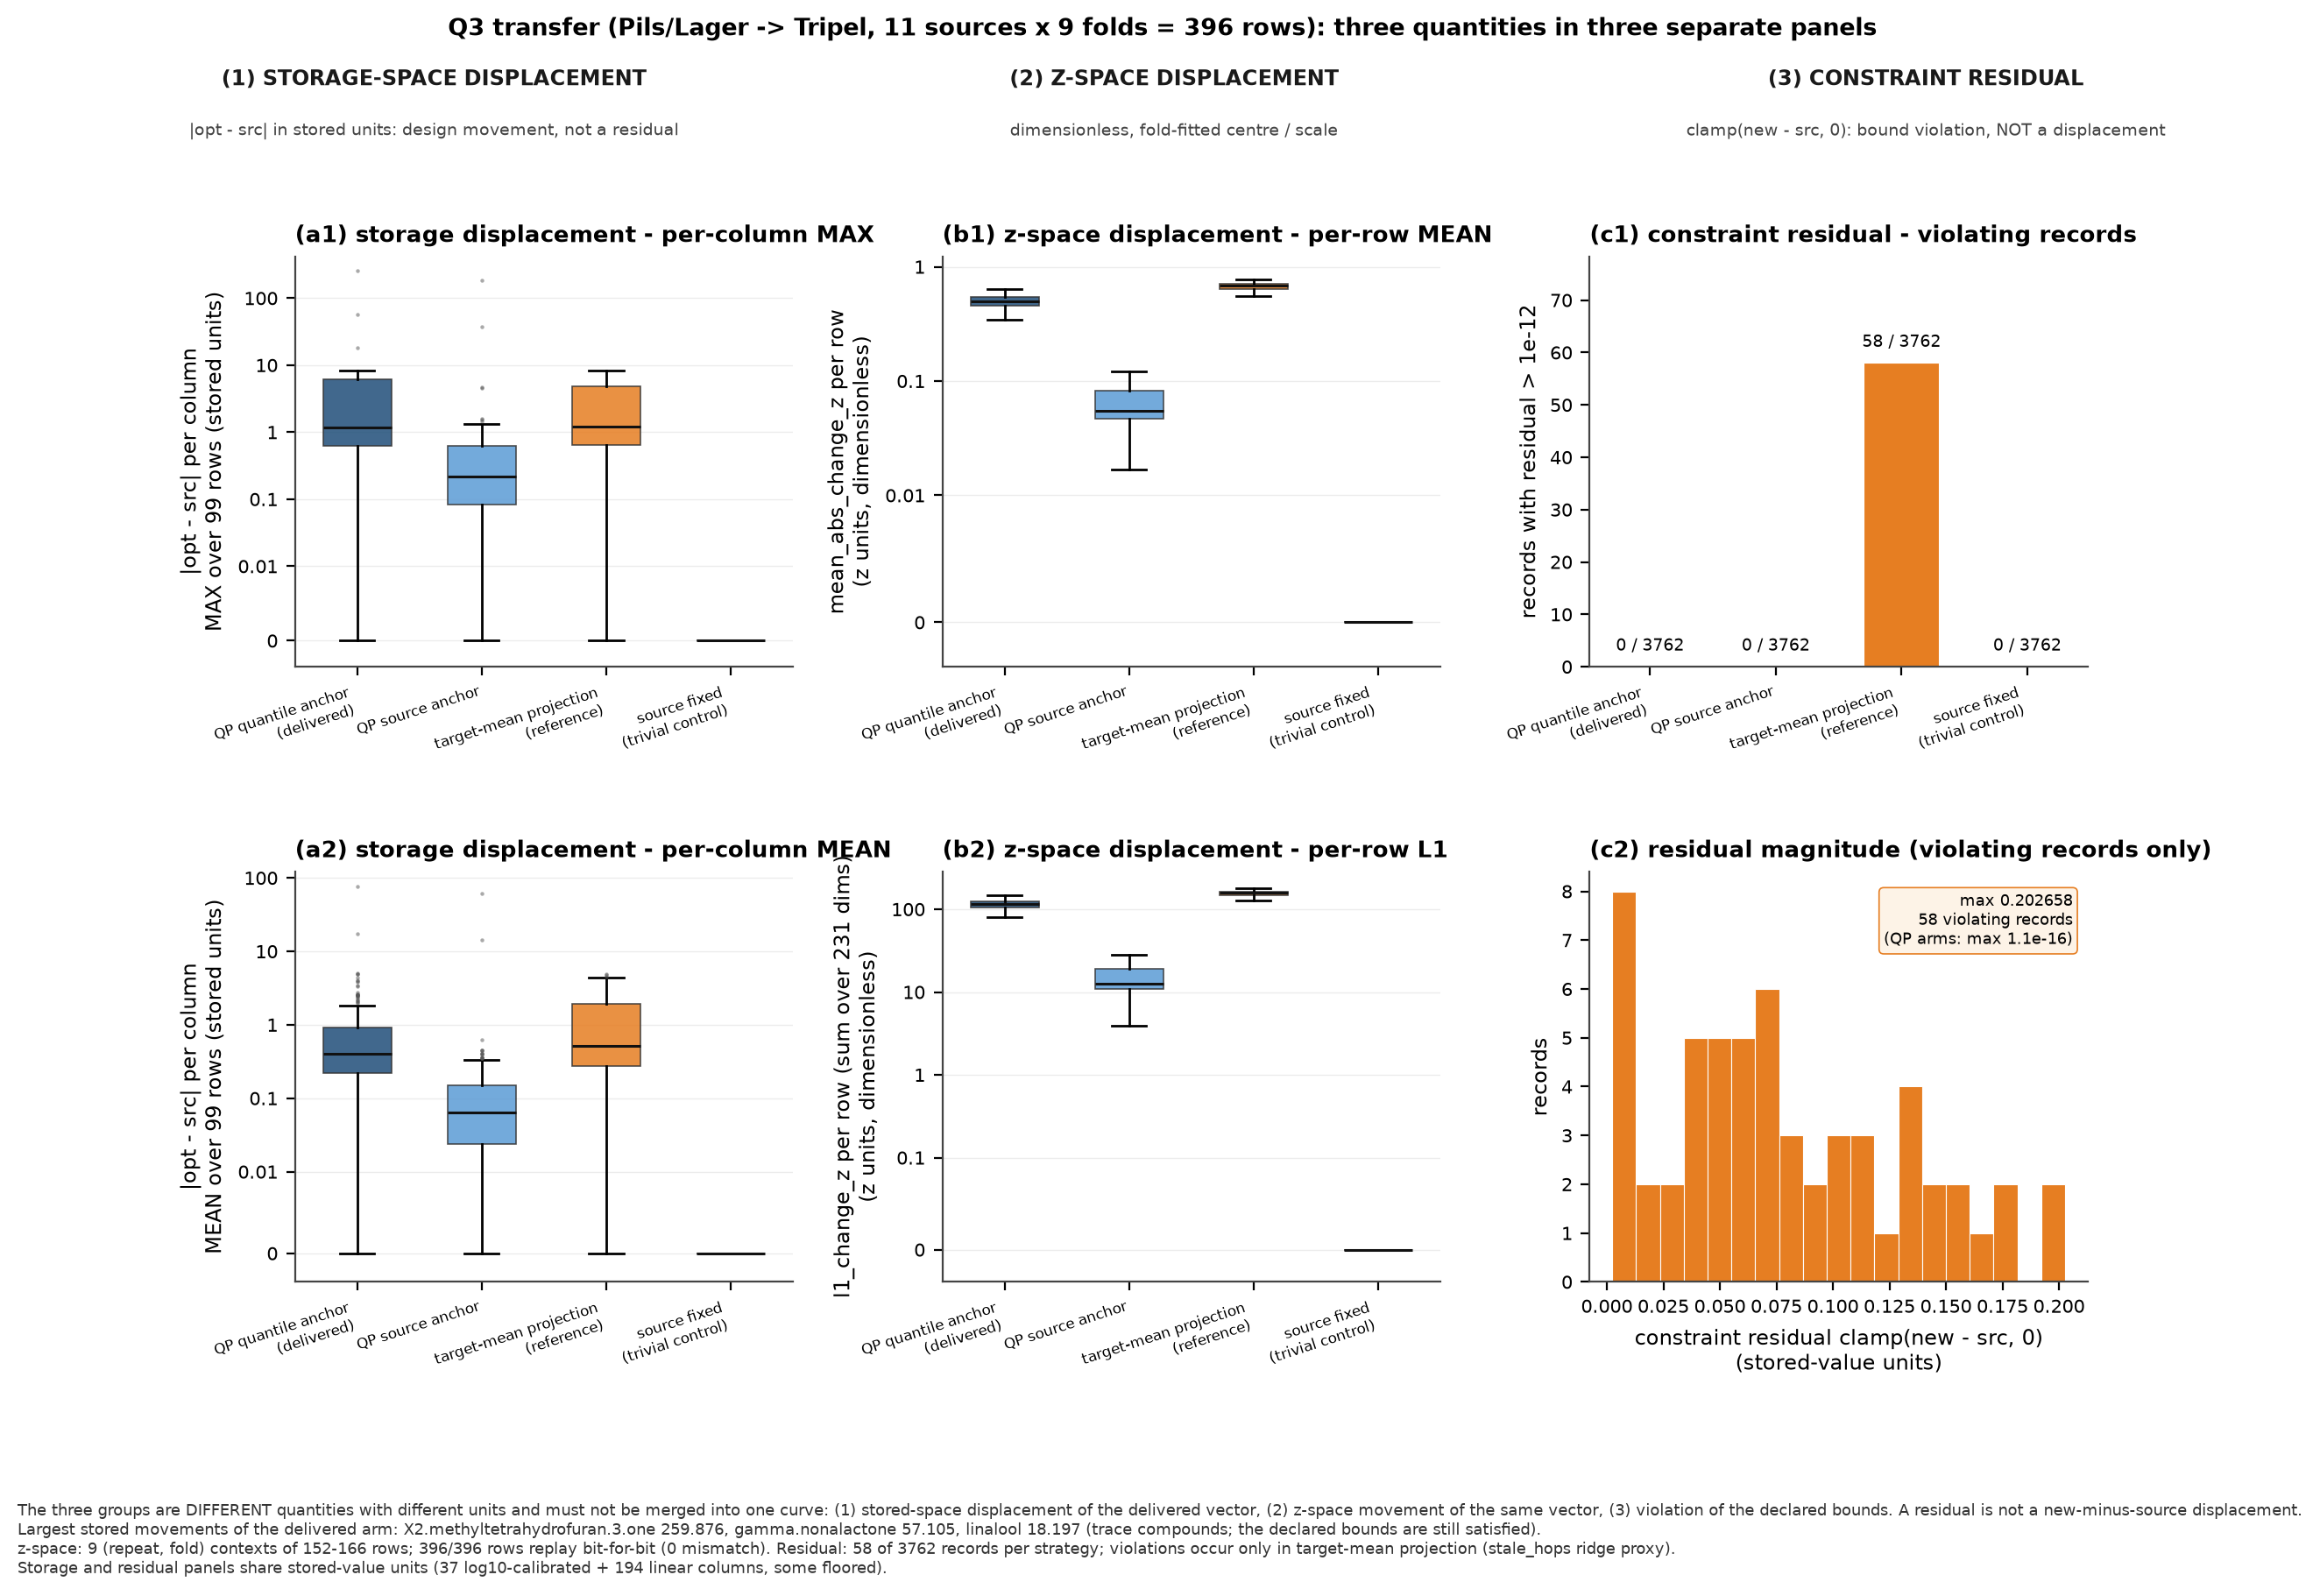
\includegraphics[width=0.92\linewidth,height=0.42\textheight,keepaspectratio]{../figures/confirmatory/Q3-transfer-shift.png}
\captionof{figure}{问题三：迁移三组量分面板——存储位移 |opt−src|、z 空间位移、约束残差 clamp(new−src,0)；残差非位移，按策略区分。（\texttt{FIG-0039}）}
\end{bpfigure}

另外，目标风格参照的自距为
4.74908413763155e-16，即参照点与自身距离在数值零处；先导轮曾因未减去目标均值而使该自距明显非零，本轮已修正为数值零。迁移前后的分布变化以分布能量衡量：迁移谱能量
2.261080494465066，源点固定对照 7.196326285149654，目标均值投影对照
6.94148284204317。

\subsection{问题三的作用边界}\label{ux95eeux9898ux4e09ux7684ux4f5cux7528ux8fb9ux754c}

第一，迁移是``声明模型下的最优''，不是真实迁移。结论只在 231 维 z
空间、声明的盒界与单条代理半空间、以及``秩 10 二次目标 + \(\lambda\)
锚点项 + \(L_1\)
项''这一目标函数下成立；它不是全局最优、不是迁移准确率，也不是原生优化验证项。

第二，没有迁移后的真实标签。迁移结果只能与``目标风格训练统计量''比较，任何``更接近真实
Tripel
风味''的表述都超出证据；本文只报告目标距离与约束状态，不报告准确率。

第三，生成不等于优于参照。设计谱在能量距离口径下劣于源样本重采样参照，本文不宣称生成模型优于基线，也不宣称其无条件的分布保真。

第四，\texttt{source-fixed} 这类平凡对照与 QP
结果必须分开呈现；不增率的饱和性使该指标无法区分``有改善''与``未移动''。

第五，双对象限制仍然存在：单一选择字段只能表示生成侧组件，迁移组件只能由理由文本与断点文档登记，因此本问的选择状态为草稿选择。

\section{稳健性与限制}\label{ux7a33ux5065ux6027ux4e0eux9650ux5236}

\subsection{检验设计}\label{ux68c0ux9a8cux8bbeux8ba1}

稳健性检验在主方案确定之后、且在任何比较之前预注册：先登记评价指标、扰动清单与判定规则，再执行扰动实验。判定量为相对极差

\[\bpMathFit{
R=\frac{\max m-\min m}{\max(|m_{\mathrm{ref}}|,10^{-12})},
}\]

其中 \(m_{\mathrm{ref}}\)
为参考运行（扰动前的对照）指标。四个问题对象各有独立计划、独立上限，不合并判定。

需要先说明一处口径历史：部分计划记录里的 reference
字段是自由文本，插件按分母为 1 计算，因此记录里的``relative
spread''实际是\textbf{绝对极差}。本文在每条检验中把绝对极差与真实相对极差分列，并以真实相对极差对照上限；该口径修正记录在结论层，不修改历史记录。

\subsection{分列的四组检验}\label{ux5206ux5217ux7684ux56dbux7ec4ux68c0ux9a8c}

\begin{bptable}
\setcounter{table}{14}
%% table-id: rob-confirmatory sha256:30a93c3f2a1d383a2af6303d74f3e76da0e5b92788b18b4637a90a0b14331ed2
\captionof{table}{四组稳健性检验的实际范围}\label{tab:rob-confirmatory}
\par\smallskip
\small
\begin{tabular}{@{}>{\raggedright\arraybackslash}p{\dimexpr 0.0718\linewidth-6pt\relax}>{\raggedright\arraybackslash}p{\dimexpr 0.1839\linewidth-6pt\relax}>{\raggedleft\arraybackslash}p{\dimexpr 0.1014\linewidth-6pt\relax}>{\raggedleft\arraybackslash}p{\dimexpr 0.0855\linewidth-6pt\relax}>{\raggedleft\arraybackslash}p{\dimexpr 0.0855\linewidth-6pt\relax}>{\raggedright\arraybackslash}p{\dimexpr 0.1445\linewidth-6pt\relax}>{\raggedright\arraybackslash}p{\dimexpr 0.0404\linewidth-6pt\relax}>{\raggedright\arraybackslash}p{\dimexpr 0.0634\linewidth-6pt\relax}>{\raggedright\arraybackslash}p{\dimexpr 0.1914\linewidth-6pt\relax}@{}}
\toprule
稳健性检验 & 对象与指标 & 三值 & 绝对极差 & 真实相对极差 & 判定规则与上限 & 判定 & 扰动方法 & 限制 \\
\midrule
问题一稳健性检验 & 问题一候选模型的 A/\allowbreak{}F30 等权 MAE & 0.3542 /\allowbreak{} 0.3624 /\allowbreak{} 0.3576 & 0.0082 & 0.0232 & 相对极差 ≤ 0.0500（relative-\allowbreak{}range） & 通过 & 多种子 + 参数扰动 & 只覆盖两次冻结重复，且参数扰动只改内层正则网格的 λ 倍数。 \\
问题二稳健性检验 & 问题二 Top-3 平均两两 Jaccard & 0.2103 /\allowbreak{} 0.2073 /\allowbreak{} 0.2053 & 0.0050 & 0.0238 & 相对极差 ≤ 0.1000（relative-\allowbreak{}range） & 通过 & 多种子 + 预算扰动 & 只覆盖两次冻结重复；bootstrap 预算由 500 降到 200 会同时降低蒙特卡洛精度。 \\
问题三生成稳健性检验 & 问题三生成谱的归一化能量距离 & 0.8778 /\allowbreak{} 0.8765 /\allowbreak{} 0.8982 & 0.0217 & 0.0247 & 相对极差 ≤ 0.0500（relative-\allowbreak{}range） & 通过 & 多种子 + 参数扰动 & 只覆盖两次冻结重复；参数扰动只改边际收缩的 κ 网格。 \\
问题三迁移稳健性检验 & 问题三迁移的综合不增率（四条化学列 + 老化酒花代理合计口径；旧称逐列不增率） & 1.0000 /\allowbreak{} 1.0000 /\allowbreak{} 1.0000 & 0.0000 & 0.0000 & 每个取值须 ≥ 1（min-\allowbreak{}value） & 通过 & 多种子 + 参数扰动 & 指标有界且饱和（三次均为 1），只能说明没有变差，不能读成强稳健。 \\
\bottomrule
\end{tabular}
\begin{tablenote}注：每行是一次预注册的稳健性检验，三值分别对应参考运行、种子扰动运行与参数/预算扰动运行。绝对极差为三值最大值减最小值；真实相对极差为绝对极差除以参考值——台账早期把绝对极差记作 relative spread（分母按 1 计），本表按真实分母重算并在第四、五列分列。判定规则与上限在比较之前登记；问题三迁移用 min-value 规则，因指标有界饱和，1.0 是构造上界。所有判定只描述本组扰动，不构成模型全面稳定的证据。\end{tablenote}
\end{bptable}

\textbf{问题一。} 参考运行、种子扰动与参数扰动的 Aroma/Flavour 30 维等权
MAE 分别为
0.35422354618559243、0.36243390816790516、0.35763459908881995；参数扰动只把内层
\(\lambda\) 网格整体乘以 0.5。绝对极差与相对极差见上表，判定上限为
0.05。

这一组必须附带一条来源说明：该检验属\textbf{来源一致性修复后的重登记}，不是首次预注册。先导轮的同名计划与其记录仍按历史保留，三组扰动值与旧记录逐位相同；重登记的目的是把三条实验统一到同一版封装代码（同一代码身份），因此本组只证``当前协议下一致''，不能读作一次新的独立稳健性证据。这也正是本文把该组与其余三组分开列出的原因。

\textbf{问题二。} 参考运行、种子扰动与预算扰动的 Top-3 平均 Jaccard
分别为
0.2103333333333333、0.20733333333333334、0.20533333333333334；预算扰动把
bootstrap 由 500 次降为 200 次，判定上限为 0.10。这一组的极差里混有
Monte-Carlo
精度变化，因此它检验的是``流程对该预算是否敏感''，而不是纯粹的``候选选择是否稳定''。

\textbf{问题三·生成。}
参考运行、种子扰动与参数扰动的归一化能量距离分别为
0.8777844056665478、0.876453018856588、0.8981550487535501，参数扰动改变
Copula 收缩参数网格，判定上限为
0.05。判定只使用分布质量指标；约束满足率恒为 1
的构造量不参与稳定性判定。

\textbf{问题三·迁移。}
参考运行、种子扰动与目标函数权重扰动的综合不增率（旧称逐列不增率）分别为
1、1、1，判定规则为``每次运行都必须保持
1.0''。由于该指标有界且饱和，三次均为 1
的结果\textbf{不构成改善或强稳健性证据}，只能说明约束在三种设置下都被构造性满足。

\begin{bpfigure}
%% figure-id: FIG-0040 sha256:ab3461581ee902afde41bf6897316b67f8f9aedac12035919cdf6ec85f05be70
%% figure-src: ../figures/confirmatory/ROB-summary.png
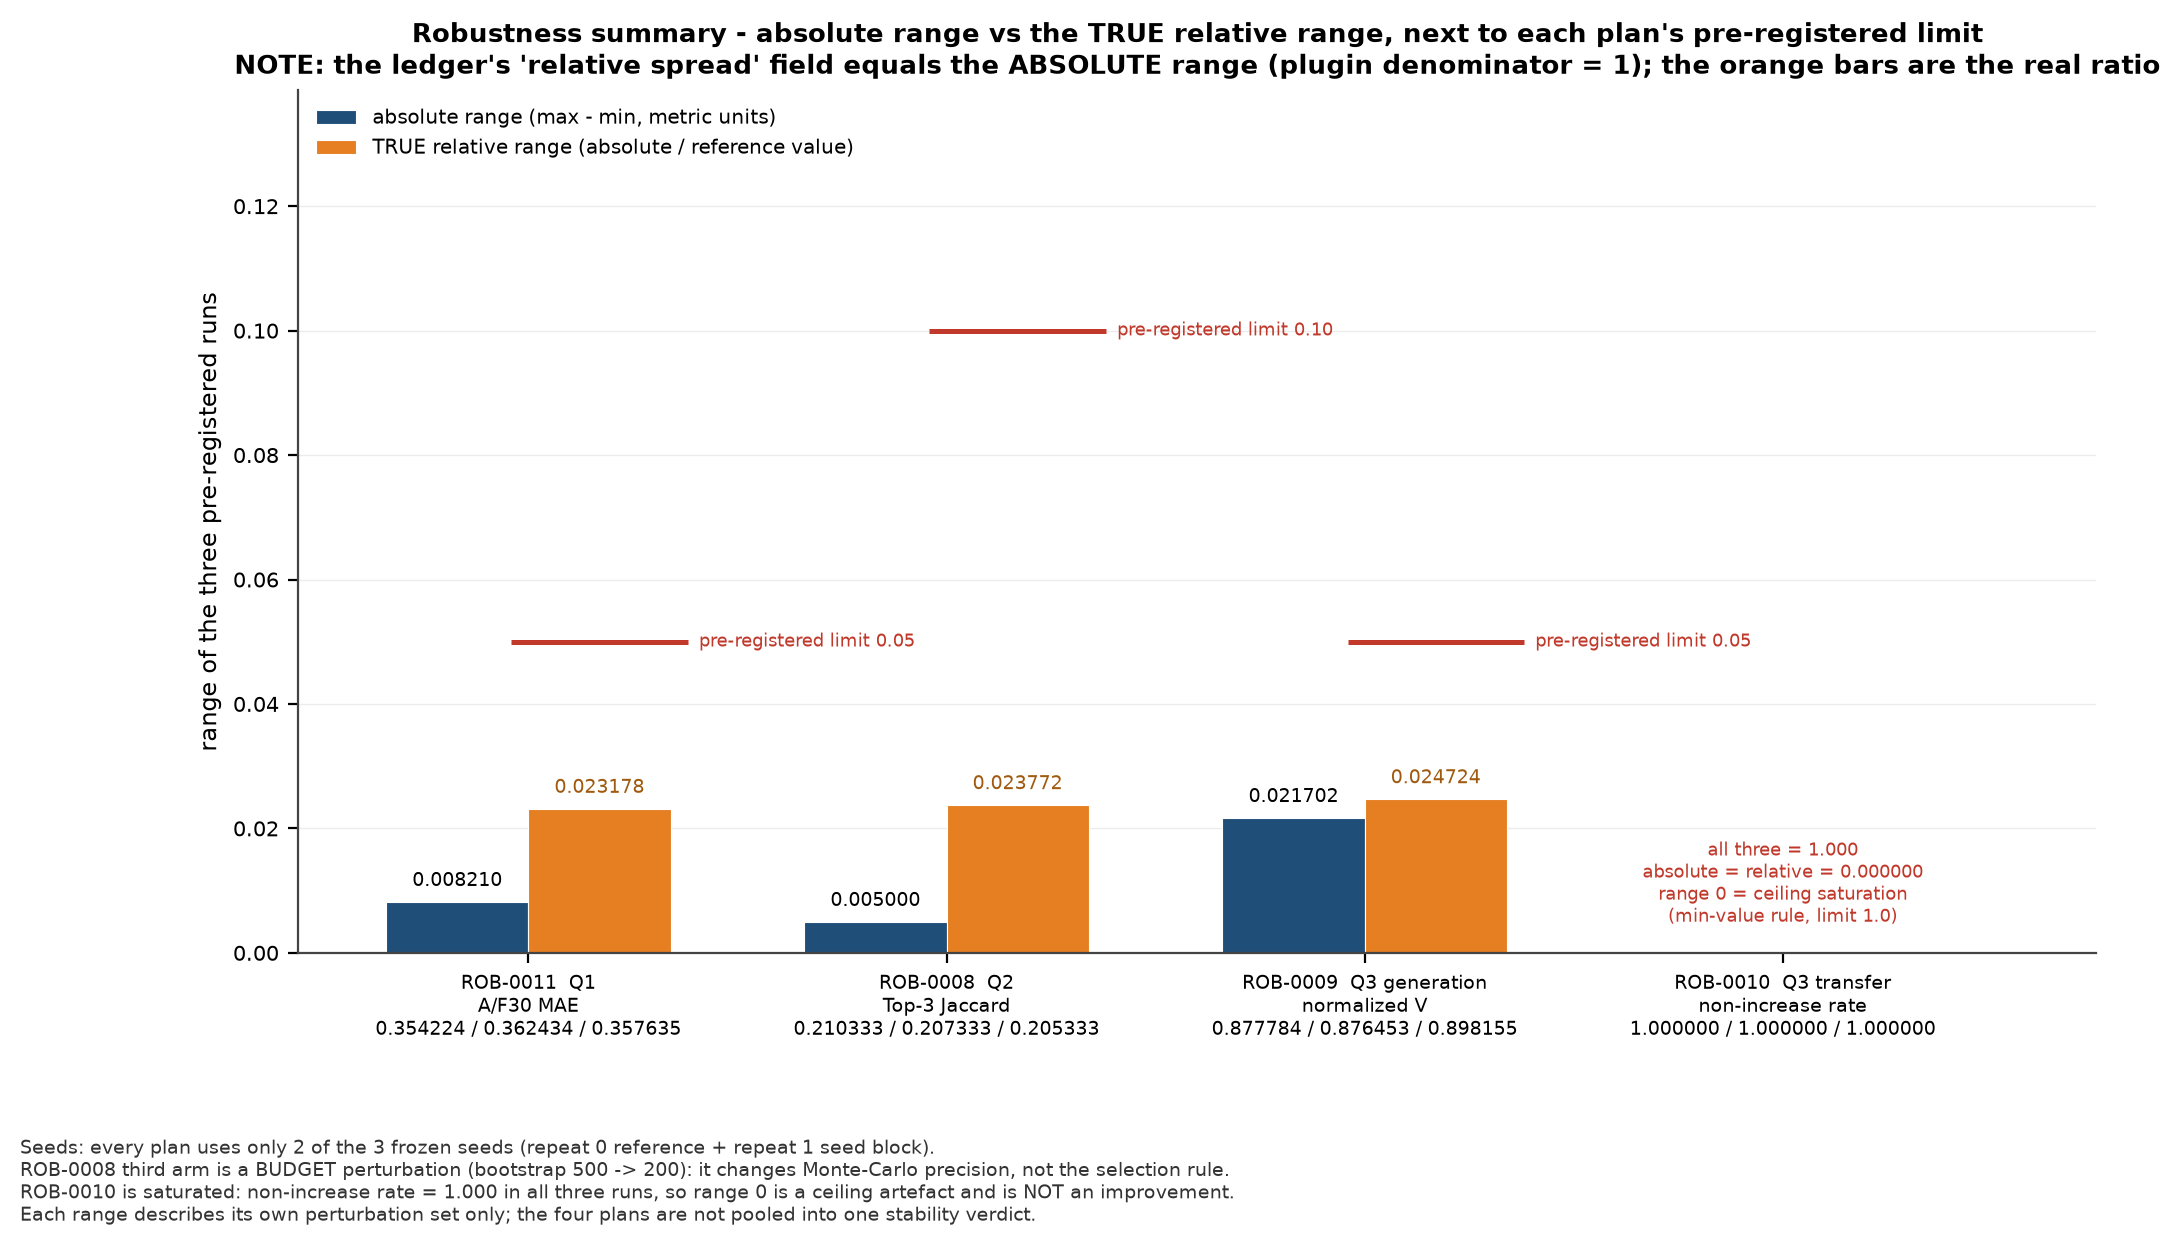
\includegraphics[width=0.92\linewidth,height=0.42\textheight,keepaspectratio]{../figures/confirmatory/ROB-summary.png}
\captionof{figure}{四组稳健性：绝对极差与真实相对极差并排、各自预注册上限；仅2/3冻结种子，含预算扰动与迁移侧饱和（极差0非改善）。（\texttt{FIG-0040}）}
\end{bpfigure}

\subsection{这些检验没有覆盖什么}\label{ux8fd9ux4e9bux68c0ux9a8cux6ca1ux6709ux8986ux76d6ux4ec0ux4e48}

第一，四个对象都只执行了三个冻结种子中的两个（重复 0 与重复
1），第三组仅记录在计划中而未执行。因此任何``种子稳健''的说法都只覆盖
2/3 的冻结种子。

第二，参数扰动只沿单一方向的小幅改动（\(\lambda\) 网格乘 0.5、Copula
收缩参数换档、目标函数 \(L_1\)
权重加倍），不是参数空间的系统扫描；不能据此断言``参数不敏感''。

第三，固定种子的独立复跑与外层实验逐位一致，这只证明\textbf{确定性重现}，不是独立实现，也不增加独立样本量。问题一的复跑容差为
\(10^{-9}\) 量级。

第四，四组检验的对象、指标与上限都不同，不能合并成``模型全面稳定''的单一结论。问题三的生成侧与迁移侧尤其不可合并：两者的指标一个衡量分布差异、一个衡量约束状态，连数值量纲都不同。

第五，部分题目要求项因证据不足被登记为``数据不足''，\textbf{不是通过}。具体包括：多阈值迁移情景与
Pareto 权衡缺少可核对证据；交付门禁未通过（质量检查仍有
\texttt{needs\_review}
与结构性不可满足项，交付冻结被工具具名拒绝）；图表标注与结论的逐项一致性仍属人工判断。这三项在本稿中如实保留为未完成，不以文件存在冒充覆盖。

\section{组件作用与负结果汇总}\label{ux7ec4ux4ef6ux4f5cux7528ux4e0eux8d1fux7ed3ux679cux6c47ux603b}

本文的组件对照分散在四张表中，此处只作整合，不重复数值。

\textbf{预测结构（表 q1-models）。} 图 Ridge 与普通 Ridge
的误差几乎相同，说明仅加入图正则不足以改变结果；图低秩相对普通 Ridge
的改善也小于与中位数基线的差距。因此图与低秩的作用应定位为提供多输出共享结构、共线性去噪与可解释系数，而不是提供稳定领先的预测增益。这是一个负结果，本文不通过挑选有利的折或维度来弱化它。

\textbf{关联识别（表 q2-stability）。}
四种方法之间的集合一致性低于三次重复之间的一致性，说明候选名单主要受方法口径影响；符号一致性均值显示约四分之一的（候选，维度）组合在重抽样下改变方向。Top-3
因此应读作``排序假设''，而不是``已识别的关键化合物清单''。

\textbf{生成对照（表 q3-quality）。}
约束投影的分布代价很小（原始抽样与设计谱的归一化能量距离几乎相同），但这不改变一个更基本的结论：生成设计谱在本口径下劣于源样本重采样参照。三类
Copula
收缩方案之间的差异小于它们与重采样参照的差异，说明在本数据上``依赖结构怎么估''不是主导误差来源；边际误差本身仍然可观。

\textbf{迁移对照（表 q3-transfer-stages）。} \texttt{source-fixed}
平凡对照的不增率同为
1，说明该指标无法区分``有改善''与``未移动''；\texttt{target-\allowbreak{}mean-\allowbreak{}projection}
参照控制的综合不增率明显低于 1（表 q3-transfer-stages），且该低值完全由
\texttt{stale\_hops} 代理上限越界造成、四条化学 cap 仍全为
1；也就是说，真正有约束力的是代理上限，而不是三条物理缺陷阈值。两者并置才是这一组实验的真正信息量。

\section{结论、建议与局限}\label{ux7ed3ux8bbaux5efaux8baeux4e0eux5c40ux9650}

\subsection{主要结论}\label{ux4e3bux8981ux7ed3ux8bba}

本文以可核实的尺度字典统一连接感官预测、因素识别与风格生成，并在每一问内先固定协议、后比较候选。

问题一在同一嵌套协议下比较了四个模型。图正则低秩模型的 Aroma/Flavour 30
维等权平均绝对误差为 0.35929156588219174，同协议中位数基线为
0.39817732837288883，全部 50 维为 0.350504156920024（基线
0.3918800487369867）；全部预测为折外预测，0--6
等级为训练分布内标定的相对等级。图正则与低秩两个组件单独的作用有限，本文明确不声称其具有稳定领先优势。

问题二在严格单体化合物与扩展指标分表的口径下给出逐维 Top-3。四种方法
Top-3 的平均两两 Jaccard 为 0.2091111111111111，候选入选频率均值为
0.42045666666666665，说明单维候选仍存在实质竞争；该量是集合一致性而非准确率，交叉相关表对照属同源核对而非外部验证。

问题三在生成与迁移两个对象上分别给出结论。生成侧的设计谱归一化能量距离为
0.8840256215416039，但源样本重采样参照更低（表
q3-quality），生成器未超过该参照；三风格单独池化值明显高于 21
风格池化值（表
q3-quality），两者不得互相替代。迁移侧在声明的凸二次规划下 198
次求解全部最优，综合不增率（旧称逐列不增率）为
1，但该值是构造上界且已饱和，不能作为改善证据。

\subsection{实践建议}\label{ux5b9eux8df5ux5efaux8bae}

面向配方筛选，应先用 Top-3
与共表达网络定位候选组合，再用小规模酿造或加标实验检验机制；本文的候选排序不构成因果证据，不能直接指导添加量。

面向风格设计，可把真实目标风格的酯类、高级醇与酸类范围作为参考，同时对
DMS、双乙酰、4VG 与反式-2-壬烯醛保留逐样本阈值核验。对 Kriek、Lambic
等小样本风格，生成结果的质量明显弱于整体水平，应用时应优先补充样本与人工品评，而不是直接采用生成均值作为配方目标。

面向预测交付，0--6
等级只能作为同数据内的相对排序使用；若需要与人工评分可比，必须取得原始评分与量表标定参数，并重新做一致性检验。

\subsection{适用边界}\label{ux9002ux7528ux8fb9ux754c}

本稿是论文源工作稿，不是最终提交版，具体边界如下。

第一，证据层级不齐。问题一的划分完整性与留出指标检查结构性不可满足，选择状态为草稿选择；问题三的原生优化可行性与优化目标检查被工具具名拒绝，本文不声称通过；问题二虽为已验证选择，但其核心量的语义是集合一致性而非准确率。

第二，0--6
等级未恢复人工评分。附件评分工作簿为空白模板，级别由训练折经验分布标定，预测向中部收缩，整级一致率与二次加权
\(\kappa\) 因此受限。

第三，关联与迁移都不涉及因果。问题二为同期关联，问题三为声明模型下的优化结果且无迁移后真实标签；两者都不支持``机制已被证实''的表述。

第四，稳健性覆盖不全。四组检验只覆盖 2/3
冻结种子；参数扰动为单方向小幅改动；固定种子复跑仅证确定性重现；迁移侧指标饱和使极差为零无法解释为稳健。

第五，附件之间同源，不能互为独立验证；六大来源的交叉相关表对照只能核对接径，不能代替外部数据。

\section*{参考文献}\label{ux53c2ux8003ux6587ux732e}
\addcontentsline{toc}{section}{参考文献}

{[}1{]} 2026 年 MathorCup 数学应用挑战赛------大数据竞赛. 赛道
A：啤酒酿造化合物分析与啤酒风味预测：初赛题面及附件 1--8. 2026.

{[}2{]} Schreurs M, Piampongsant S, Roncoroni M, et al.~Predicting and
improving complex beer flavor through machine learning. \emph{Nature
Communications}, 2024, 15: 2368.
\href{https://doi.org/10.1038/s41467-024-46346-0}{doi:10.1038/s41467-024-46346-0}.

{[}3{]} Gibson B, Vidgren V, Peddinti G, Krogerus K. Diacetyl control
during brewery fermentation via adaptive laboratory engineering of the
lager yeast \emph{Saccharomyces pastorianus}. \emph{Journal of
Industrial Microbiology \& Biotechnology}, 2018, 45: 1103--1112.
\href{https://doi.org/10.1007/s10295-018-2087-4}{doi:10.1007/s10295-018-2087-4}.

{[}4{]} Baldus M, Klie R, Biermann M, et al.~On the Behaviour of
Dimethyl Sulfoxide in the Brewing Process and its Role as Dimethyl
Sulfide Precursor in Beer. \emph{BrewingScience}, 2018, 71(1/2): 1--11.
\href{https://doi.org/10.23763/BrSc18-01baldus}{doi:10.23763/BrSc18-01baldus}.

\newpage
\appendix

\section*{附录 A　逐维误差、逐风格与完整
Top-3（完整表见支撑材料）}\label{ux9644ux5f55-a-ux9010ux7ef4ux8befux5deeux9010ux98ceux683cux4e0eux5b8cux6574-top-3ux5b8cux6574ux8868ux89c1ux652fux6491ux6750ux6599}
\addcontentsline{toc}{section}{附录 A　逐维误差、逐风格与完整
Top-3（完整表见支撑材料）}

\textbf{Aroma/Flavour 逐维误差（按 Skill 升序）}见支撑材料
\texttt{report/\allowbreak{}tables/\allowbreak{}q1-\allowbreak{}targets.md}（同数据 \texttt{.csv}）：含 30
维逐维候选 MAE、中位数基线 MAE、差值与 Skill，\textbf{恶化维度（Skill
为负）逐条保留}，未删任何行。正文给出 A/F30 与分组的汇总结论。

\textbf{逐风格误差与样本量（22 个风格）}见支撑材料
\texttt{report/\allowbreak{}tables/\allowbreak{}q1-\allowbreak{}styles.md}（同数据
\texttt{.csv}）：小样本风格（Faro 3 款、Brut 4 款、Flanders old brown
5、Scotch
5）的高误差行逐条保留。正文只陈述``小样本风格误差明显更大''这一汇总结论。

Skill
为负的维度表示该维上模型劣于逐目标训练中位数；这些维度多为训练样本极少的缺陷或风格特定维度。汇总
Skill 为正不能掩盖它们的恶化。

\textbf{完整 50 维 Top-3（每维 3 项，共 150
条目）}见支撑材料：\texttt{report/\allowbreak{}tables/\allowbreak{}q2-\allowbreak{}full-\allowbreak{}top3.md}（同数据
\texttt{report/\allowbreak{}tables/\allowbreak{}q2-\allowbreak{}full-\allowbreak{}top3.csv}）。该表已从正文移出以控制篇幅；其输入路径、输入/输出
SHA 与表→实验映射记录在表格索引
\texttt{report/\allowbreak{}tables/\allowbreak{}INDEX.json}，数据行未做任何删减。正文只保留核心维度表
q2-core-top3 与稳定性汇总。

\(\pi\) 为风格分层 bootstrap 的入选频率，\(S\)
为原样本综合百分位分数，方向取总体 Spearman
符号。``类别''按绝对关联强度分类，不能读作已检验所有风格内方向相同。维度编码保持与原始感官表一致：\texttt{A\_}
为 Aroma，\texttt{F\_} 为 Flavour，其余为口感、缺陷及总体评价。

\textbf{扩展候选宇宙（15 个非单体指标）在 50 个感官维度上的
Top-3}见支撑材料：\texttt{report/\allowbreak{}tables/\allowbreak{}q2-\allowbreak{}extended.md}（同数据
\texttt{report/\allowbreak{}tables/\allowbreak{}q2-\allowbreak{}extended.csv}）。移出原因同为篇幅，不表示证据缺失；同样在
\texttt{report/\allowbreak{}tables/\allowbreak{}INDEX.json} 中有完整溯源。

扩展表与严格表分开报告，是因为这些指标是组成或工艺标志，不是单一挥发性风味分子。

\section*{附录
B　复现要点}\label{ux9644ux5f55-b-ux590dux73b0ux8981ux70b9}
\addcontentsline{toc}{section}{附录 B　复现要点}

\subsection*{B.1
计算与复核顺序}\label{b.1-ux8ba1ux7b97ux4e0eux590dux6838ux987aux5e8f}
\addcontentsline{toc}{subsection}{B.1 计算与复核顺序}

计算环境为项目绑定的 Python 3.12 环境，含 NumPy、pandas、SciPy 与
scikit-learn。主随机种子与三次重复的种子在协议中冻结；问题一使用全样本
3×3×3 嵌套交叉验证，问题二只在注册的 200 行训练集内进行 500
次风格分层重采样，问题三使用固定 3
折风格内留出，并按生成、迁移分别汇总。

复核顺序为：按 \texttt{beer}
对齐附件；核对校准字典与缺失计数；仅在训练折拟合预处理、图与超参数；计算折外预测与相对等级；按名称对齐交叉相关表并计算四种方法的
Top-3 与 bootstrap
频率；逐折选择生成参数并生成原始抽样与约束设计谱；在声明 QP
下求解并写证书；最后按四组独立计划执行稳健性检验。

\subsection*{B.2
脚本与产物索引}\label{b.2-ux811aux672cux4e0eux4ea7ux7269ux7d22ux5f15}
\addcontentsline{toc}{subsection}{B.2 脚本与产物索引}

本文全部数值来自项目台账登记的实验产物与由这些产物生成的表格，不在正文手抄。表格由脚本从台账指向的当前产物生成，每张表的输入路径、输入与输出
SHA-256、表到实验的映射记录在表格索引文件中；若某张表的输入缺失或指标键不存在，生成脚本会具名失败而不是填零或回退到旧实验。

\subsection*{B.3 本稿的待补项（DRAFT
状态声明）}\label{b.3-ux672cux7a3fux7684ux5f85ux8865ux9879draft-ux72b6ux6001ux58f0ux660e}
\addcontentsline{toc}{subsection}{B.3 本稿的待补项（DRAFT 状态声明）}

以下事项在本稿中\textbf{未完成}，不得以本稿冒充最终交付：

\begin{enumerate}
\def\labelenumi{\arabic{enumi}.}
\tightlist
\item
  图件已在本稿登记并进入正文：图 1--9 依次对应台账
  \texttt{FIG-0032}--\texttt{FIG-0040}，题注给出中文说明与登记编号，9
  个图像文件的 SHA-256 与台账登记值逐一一致。图 1、图 2 与图 9
  的图内英文标注在低分辨率下偏小，核对时请以登记文件原图为准。
\item
  本稿按 DRAFT
  交付：正式渲染与产物绑定已执行，但交付检查未通过最终门禁（质量检查仍有
  \texttt{needs\_review}
  与结构性不可满足项，指标复算因未登记数据划分而无法取得权威测试真值），因此本稿不冒充最终提交版；冻结身份与打包状态以交付说明（\texttt{DELIVERY-\allowbreak{}NOTES.md}）为准。
\item
  验证检查点仍不完整：问题一的划分完整性与留出指标、问题三的原生优化可行性与优化目标为结构性未通过，对应选择状态为草稿选择。
\item
  部分题目要求项登记为``数据不足''，不等于已完整回答。
\end{enumerate}

\section*{附录
C　证据类型、验证状态与限制}\label{ux9644ux5f55-c-ux8bc1ux636eux7c7bux578bux9a8cux8bc1ux72b6ux6001ux4e0eux9650ux5236}
\addcontentsline{toc}{section}{附录 C　证据类型、验证状态与限制}

本附录用人类可读的方式说明各章结论的\textbf{证据类型}与\textbf{适用限制}，不重复展开台账记录原文（含工程编号的结论原文属核对材料，随支撑材料归档，不进入正文）。

{
\begin{longtable}[]{@{}
  >{\raggedright\arraybackslash}p{(\linewidth - 8\tabcolsep) * \real{0.2000}}
  >{\raggedright\arraybackslash}p{(\linewidth - 8\tabcolsep) * \real{0.2000}}
  >{\raggedright\arraybackslash}p{(\linewidth - 8\tabcolsep) * \real{0.2000}}
  >{\raggedright\arraybackslash}p{(\linewidth - 8\tabcolsep) * \real{0.2000}}
  >{\raggedright\arraybackslash}p{(\linewidth - 8\tabcolsep) * \real{0.2000}}@{}}
\toprule\noalign{}
\begin{minipage}[b]{\linewidth}\raggedright
章节
\end{minipage} & \begin{minipage}[b]{\linewidth}\raggedright
结论类型
\end{minipage} & \begin{minipage}[b]{\linewidth}\raggedright
证据范围
\end{minipage} & \begin{minipage}[b]{\linewidth}\raggedright
验证状态
\end{minipage} & \begin{minipage}[b]{\linewidth}\raggedright
关键限制
\end{minipage} \\
\midrule\noalign{}
\endhead
\bottomrule\noalign{}
\endlastfoot
§4 预测 & 同期关联（内部分布内预测） & 同一批 250 款啤酒的折外预测 &
泄漏检查、基线比较、固定种子独立复跑通过 &
无留出集；划分完整性与留出指标检查结构性不可满足；选择为草稿选择 \\
§4 预测 & 相对分级一致性 & 训练折经验分布标定的 0--6 等级 & 与预测同协议
& 0--6 为相对等级，未恢复原始人工评分；预测向中部收缩 \\
§5 关键因素 & 同期关联（非因果） & 注册的 200 行训练集，风格分层重抽样 &
泄漏检查与固定种子独立复跑通过 &
方法间集合一致性不等于准确率；附件交叉相关表与本研究同源；方向稳定性有限 \\
§6 生成 & 描述性分布质量 & 21 个可估风格、177 个可估格 &
泄漏检查与复跑通过；原生优化检查不适用 &
生成未优于同量源样本重采样参照；三风格单独池化值不得被池化值替代 \\
§6 迁移 & 声明模型下的最优 & 231 维标准化空间、声明盒界与单条代理半空间
& 求解证书最优并经独立复算；原生优化检查未通过、不声称 &
非全局最优、非迁移准确率；无迁移后真实标签 \\
§7 稳健性 & 描述性（受预算/饱和限制） & 四个对象各自独立计划，各 2/3
冻结种子 & 判定规则在执行前登记，四组均满足 &
覆盖率不足；预算扰动降低蒙特卡洛精度；迁移侧指标饱和使极差为零不构成改善 \\
\end{longtable}
}

\textbf{未完成事项（DRAFT 状态）}：图件已与本稿同批登记并进入正文（图
1--9 =
\texttt{FIG-0032}--\texttt{FIG-0040}）；正式渲染与产物绑定已执行，但交付检查未通过最终门禁（质量检查仍有
\texttt{needs\_review}
与结构性不可满足项）；验证检查点仍不完整（问题一划分完整性/留出指标、问题三原生优化检查结构性未通过）；部分题目要求项登记为``数据不足''，不等于已完整回答。
\end{document}
